\documentclass[a4paper, onehalfspacing, usecolor, 12pt]{bwthesisEN}
% The usecolor option sets the titles in blue, as requested by
% the Ghent University housestyle. Remove this to get a black
% and white version of things.
\usepackage[english]{babel} %Use dutch headings and titles
%-------------------------------------------------------------------------------
% FILL IN YOUR DETAILS
%
% Keep in mind that UGent doesn't use copromotors any longer. However,
% if it is required to add, please uncomment the line starting with
% \copromotor below and fill in the correct details.
%
\title{Hyperdimensional computing for protein language modeling}
\subtitle{...}
\author{Michael Fatjanov}

%\wordcount{6.431} % Fill in the number of words
\studentnr{...} % Fill in your student number

\promotor{Prof. Dr. Bernard De Baets}
\copromotor{Dr. Michiel Stock}
\tutor{Dimitri Boeckaerts}

\degree{master}
\richting{Bioinformatics}

\academicyear{2022-2023}

%-------------------------------------------------------------------------------
% The preamble. Note that the following packages are already loaded by
% the class bwthesis: geometry, amsmath, amsfonts, amssymb, graphicx,
% xcolor, ulem, setspace
% This package provides the lstlisting environment
\usepackage{textcomp}
\usepackage{subcaption}
\usepackage{listings}
\definecolor{mygreen}{rgb}{0,0.6,0}


\lstset{ %
	language=Python,                % choose the language of the code
	basicstyle=\footnotesize\ttfamily,       % the size of the fonts that are used for the code
	numbers=left,                   % where to put the line-numbers
	numberstyle=\scriptsize,      % the size of the fonts that are used for the line-numbers
	stepnumber=1,                   % the step between two line-numbers. If it is 1 each line will be numbered
	numbersep=5pt,                  % how far the line-numbers are from the code
	backgroundcolor=\color{white},  % choose the background color. You must add \usepackage{color}
	showspaces=false,               % show spaces adding particular underscores
	showstringspaces=false,         % underline spaces within strings
	showtabs=false,                 % show tabs within strings adding particular underscores
	frame=none,           % adds a frame around the code
	tabsize=2,          % sets default tabsize to 2 spaces
	captionpos=b,           % sets the caption-position to bottom
	breaklines=true,        % sets automatic line breaking
	breakatwhitespace=false,    % sets if automatic breaks should only happen at whitespace
	xleftmargin=15pt,
	xrightmargin=5pt,
	commentstyle=\color{mygreen}, %teal
	keywordstyle=\color{blue},
	stringstyle=\color{orange}       % if you want to add LaTeX within your code
} % contains settings for the package listings
% this package provides an environment for algorithms (cfr. Pseudocode)
\usepackage[ruled]{algorithm2e} 
% This package provides extra possibilities for tables
\usepackage{booktabs}
% this package is used to produce both author-date and standard numerical citations for BibTeX bibliographies
\usepackage[square, numbers]{natbib}
% This packages adds the Appendix name in the toc. See below
\usepackage[titletoc]{appendix}
\usepackage{mathtools}
\usepackage{amsmath}
\usepackage{notoccite}
\usepackage{svg}
\usepackage{minted}
\usepackage{newunicodechar}
\usepackage[font={footnotesize}]{caption}
\usepackage{tabularx}
\usepackage{makecell}
\usepackage{outlines}
\renewcommand\theadfont{\normalsize\bfseries}

\setcounter{secnumdepth}{3}
% ---- ADDITIONAL SETTINGS
\graphicspath{{Fig/}} % path to the figure directory

%-------------------------------------------------------------------------------
% The actual document
%
\begin{document}

\sloppy

% Typisch copyright voor een thesis.
% Te plaatsen juist na het titelblad.
% De namen worden automatisch ingevuld, maar 

\par\vspace*{\fill}

De auteur en promotor geven de toelating deze scriptie voor consultatie beschikbaar te stellen en delen ervan te kopi\"eren voor persoonlijk gebruik. Elk ander gebruik valt onder de beperkingen van het auteursrecht, in het bijzonder met betrekking tot de verplichting uitdrukkelijk de bron te vermelden bij het aanhalen van resultaten uit deze scriptie.

The author and promoter give the permission to use this thesis for consultation and to copy parts of it for personal use. Every other use is subject to the copyright laws, more specifically the source must be extensively specified when using results from this thesis.

\vspace{1cm}

Gent, FILL IN THE DATE % FILL IN THE CORRECT DATE

\vspace{1cm}

\begin{minipage}[t][4cm][t]{0.5\textwidth}
\raggedright
The promotor,

\vspace{2.5cm}

\insertpromotor % Change if multiple names are necessary
\end{minipage}
\begin{minipage}[t][4cm][t]{0.48\textwidth}
\raggedright
The author,

\vspace{2.5cm}

\insertauthor % change if your name should be different
\end{minipage}

\thispagestyle{empty} 


\clearpage{\pagestyle{empty}\cleardoublepage}

%------------------------------------------------------------------------
\frontmatter
\pagestyle{frontmatter} %sets headers and footers correctly

% ------------ thanks -----------
\chapter{Acknowledgements}
I am sincerely grateful to my supervisor, ir. D. Boeckaerts, whose commitment to my project extended to countless proofreadings and always being on hand to answer my relentless questions. Your guidance and dedication have been invaluable and created an enjoyable and engaging learning experience.

I would also like to extend my gratitude to my promoters, Prof. B. De Baets and dr. ir. M. Stock, who made this work possible to begin with and contributed to this work by collectively proofreading my dissertation and providing insightful ideas and suggestions. Their combined expertise, keen attention to detail, and valuable feedback have significantly elevated the quality of this work.

I must also express my heartfelt gratitude to my partner, who has provided much support and encouragement throughout this journey. Your understanding and emotional support have made this challenging process much more manageable.

To my classmates, thank you for the frequent companions of coffee machine banter. The camaraderie, discussions, and shared laughter we experienced brought light to even the most stressful of days.

Lastly, my thanks go to my family. Your ongoing support and encouragement have been greatly appreciated. Thank you for everything.

% ------------ table of contents ---------
{
	\singlespacing % to keep the TOC within boundaris
  % Remove whitespace between the sections
  \setlength{\parskip}{0ex plus 0.3ex minus 0.3ex}
	\tableofcontents
}

\addcontentsline{toc}{chapter}{Contents} %add TOC to the TOC

% ------------ Acronyms ----------

% ------------ summary ----------
\chapter[Nederlandse samenvatting]{Samenvatting}

nederlandse samenvatting





\chapter{Abstract}
This dissertation explores the implementation and application of hyperdimensional computing for protein sequence analysis. We discuss the advancements of state-of-the-art protein language models in protein structure and function predictions while raising the need for more computationally and data-efficient methods. As hyperdimensional computing is proposed as a promising avenue, its underlying principles and mathematical operations are illustrated to demonstrate the potential of hyperdimensional computing in bioinformatics research. 

We research and develop several methods to encode amino acids into hyperdimensional vectors. Of these, projecting embeddings containing biological information into hyperdimensional space has proven to be useful in subsequent analyses and prediction tasks. Utilizing the PhaLP database~\cite{phalp}, a continuously updated database of phage lytic proteins, we apply these amino acid encoding methods to develop techniques for protein sequence encodings. We demonstrate the capability of these methods to capture essential protein sequence information in hyperdimensional vectors, proving their usefulness in prediction tasks. In our classification tasks, we show that hyperdimensional-computing-based learning methods display competitive performance when compared to established machine learning methods such as random forest and XGBoost. In addition, we examine perceptron-based models for context-aware protein residue learning, utilizing neighborhood-encoded hyperdimensional vectors. Although this does not outperform current state-of-the-art models, it contributes valuable insights into the challenges faced when implementing efficient models for such tasks within the hyperdimensional computing framework. 

Finally, we acknowledge the need for continued research in refining our encoding algorithms, exploring alternative model architectures, and extending the scope of tasks and datasets. Despite mixed results, our findings lay a solid foundation for further investigation into hyperdimensional computing's potential in protein sequence research and bioinformatics.

% The following can be commented out to remove the list of figures
% and the list of tables, as specified by the guidelines of BW
% \listoffigures
% \listoftables
%-----------------------------------------------------------------------
\mainmatter
\pagestyle{mainmatter} % sets headers and footers correctly

% Here you can add more chapters in case it is needed
\chapter[Introduction]%
{Introduction}
%% Introduction
%%%%%%%%%%%%%%%
\section{Big picture and traditional bioinformatics tools for protein research}
Proteins are an essential part of molecular biology and are responsible for a wide variety of functions. Far too wide to discuss here because they are one of the building blocks that make up life, hence a lot of effort has gone towards trying to understand the functions of protein and disruptions in its mechanisms that lead to many kinds of diseases. In spite of that, for a large fraction of the approximately 20000 human proteins, the structures and functions remain still unknown. To start, proteins are composed of a linear chain of amino acids (AA) with a length ranging from 50 to tens of thousands of AAs, all connected by peptide bonds into a polypeptide. This is also referred to as the \textit{primary structure} of a protein.\cite{primstruct} A sequence of amino acids is mostly determined by the genetic code without considering post-translational and post-transcriptional modifications etc. In the genetic code of all living organisms, there are 20 different kinds of amino acids coded which make up the 'language' of proteins. The current state-of-the-art methods for the identification of protein sequences are \textit{de novo sequencing} algorithms applied to tandem mass spectrometry data.\cite{protseq}

It is intuitive to represent a protein as a sequence of letters with each letter corresponding to an amino acid. Likewise to natural languages, we can find common elements between naturally evolved proteins. These motifs and domains are essential to many biological processes and can easily be represented as words, phrases and sentences of amino acids.
A traditional task in bioinformatics and more specifically in the realm of protein sequence analyses is the quantification of the similarity between strings of sequences. Classical pairwise alignment algorithms include the algorithm of \textbf{Needleman \& Wunsch} \cite{global} for global alignments and that of \textbf{Smith \& Waterman} \cite{local} for local alignments. These algorithms are sufficient for comparing two sequences but unfeasible for searching databases for homologous sequences, hence faster algorithms like FASTA \cite{fasta} and, as of yet widely used for simple searches for similar sequences, BLAST \cite{blast} were made. A natural extension of pairwise alignment is multiple sequence alignment (MSA), which is to align multiple related sequences. This reveals much more information than pairwise alignment can. It allows for the identification of conserved sequence patterns and critical amino acid residues which is highly important for constructing phylogenetic profiles and can help in the prediction of secondary and tertiary 3-dimensional structures as we see later.

To cope with the number of recorded protein sequences rising exponentially, far more compute-wise efficient methods based on multiple sequence alignments had to be developed like PSI-BLAST \cite{psiblast}, HHblits \cite{hhblits3} and MMseqs \cite{mmseqs2}. However, these methods might not be able to keep up with the ever increasing number of protein sequences stored in databases.

A protein also consists of much more than a mere sequence, however. It is a 3-dimensional structure with a predetermined form and function. While a protein's structure and function are dynamic and dependent on its surroundings such as the cellular state and other proteins and molecules akin to natural languages, it is still defined by its underlying sequence. This means that a lot of the 3D-structural and functional information of a protein should be retrievable from its amino acid sequence.\cite{structure} The most common way to determine the 3D structure of a protein has remained to be X-ray crystallography for more than half a century \cite{xray}, with cyro-electron microscopy now catching up rapidly.\cite{cyroem} However, these kinds of laboratory approaches for structure determination of proteins are not simple, expensive and in some cases not possible for the protein in question whilst sequence determination is relatively much easier to perform.For this reason, the number of verified three-dimensional structures has not kept up with the explosive growth in sequence information. On top of that, structure prediction is highly in demand for researchers in applications such as drug design.  Therefore, a lot of effort has gone into computational methods for structure and function predictions from protein sequences.

\section{State-of-the-art protein language modeling}

\section{Hyperdimensional computing}
Hyperdimensional computing (HDC) is a relatively new paradigm of computing developed by \textbf{Kanerva} \cite{Kanerva2009} that tries to mimic the workings of a (human) brain by computing with vectors of tens of thousands of elements long, so in the realm of hyperdimensionality. The human brain consists of about 100 billion neurons (nerve cells) and 1000 trillion synapses that connect these neurons. Each neuron is connected to up to 10000 other neurons, creating massive circuits. This is likely fundamental to the workings of the human brain and what separates our brains from modern von Neumann computer architectures which operate on 8 to 64-bit vectors. This becomes clear when we compare the relative simplicity for a human to learn a language compared to computers. Computers use a large and complicated set of arithmetic operations in the form of deep learning networks which require terabytes of data and thousands of Watts of computing power to come close to mastering a language whilst a human can recognize other languages relatively easily when they don't even speak it. Likewise languages, we can very easily memorize and compare other intrinsically complex and contextual concepts such as images. A computer would have a hard time finding similarities between a set of images and faces because this requires very complex machine learning models. The human brain can do this all with a very large efficiency by consuming only roughly 20 W of energy.

Achieving these kinds of flexible brain-like models based on high dimensionality is not entirely new and is being explored since the 1990s. Some of these earlier models include Holographic Reduced Representations~\cite{HRR}, Spatter Code~\cite{spatter} etc. A hyperdimensional vector (HDV) can represent anything from a scalar number to any kind of concept. This vector is initially made up of totally random elements, but with a simple set of operations which will be explained later, we can use other vectors to combine some concepts into new similar or dissimilar concepts. For example, to show the essence of HDC and how it tries to simulate the brain, we can compare the concept of a \textit{table} to the concept of a \textit{brocolli}. We would not immediately conclude that they are in any way similar but as humans, we can trace back \textit{table} to \textit{plate} which has some similarities with \textit{food} from which we can easily extract the concept of \textit{brocolli}. These kinds of operations are not very obvious for a classical computer but creating these semantic pathways are rather easy for humans.

The elements in an HDV can be made up of binary bits like in classical computing but also of bipolar or real numbers. The choice of the nature of the elements has also implications on the nature of the different operations and the results. Highly efficient bit operations could be used on binary vectors but then the amount of information stored in such a vector would be drastically lessened compared to bipolar or real vectors, leading to lower accuracy.  

An initial HDV is made up fully randomly. This \textit{holistic} or \textit{holographic} representation of a concept smeared out over a vector consisting of thousands of bits gives rise to interesting properties such as its robustness. These kinds of systems are very tolerant to noise and failure of bits since we introduce a lot of redundancy in the vector just by stochastics. This is very unlike classical computing where every bit counts and one failure in a bit can lead to disasters. 
\subsection{Operations on hyperdimensional vectors}
The interesting properties of HDC are based on only four basic operations we can perform on HDVs. We will discuss these for bipolar and binary vectors.
\subsubsection{Similarity measurement} \label{sssec:sim}
For many kinds of problems, it will be necessary to quantify the similarity between two HDVs. The method depends on the nature of the vectors. For binary vectors, the \textit{Hamming distance} defined as in equation~\ref{eqn:Hamming} is widely used.
\begin{equation}
    \label{eqn:Hamming}
    Ham(A, B) = \frac{1}{d} \sum_{i=1}^{d} 1_{A_{(i)} \neq B_{(i)}}
\end{equation}
The \textit{cosine distance} as defined in equation~\ref{eqn:cosine} is most commonly used for bipolar vectors.
\begin{equation}
    \label{eqn:cosine}
    cos(A, B) = \frac{A \cdot B}{||A|| * ||B||}
\end{equation}
The results of both of these measurements are summarized in table~\ref{tab:dist}.
\begin{table}[h]
    \begin{tabular}{|c||c|c|c|}
        \hline
        \textbf{Measurement} & \textbf{Dissimilar} & \textbf{Orthogonal} & \textbf{Similar} \\
        \hline
        \textbf{Hamming distance} & 1 & 0.5 & 0 \\
        \hline
        \textbf{Cosine similarity} & -1 & 0 & 1 \\
        \hline
    \end{tabular}
    \caption{\label{tab:dist}Overview of similarity measurements in HDC depending on the nature of the HDVs} 
\end{table}
It is important to note that two random HDVs will be orthogonal to each other just by stochastics. Also notice that the first quantifies a distance and the latter a similarity.
\subsubsection{Addition} \label{sssec:add}
Also referred to as \textit{bundling}, the element-wise addition as in equation~\ref{eqn:sum} of $n$ input vectors $\{X_{1} + X_{2} + \cdots + X_{n}\}$ creates a vector $X$ that is maximally similar to the input vectors.
\begin{equation}
    \label{eqn:sum}
    X = X_{1} + X_{2} + \cdots + X_{n}
\end{equation}
For bipolar vectors this is straightforward. The input vectors are added element-wise but the resulting vector is restricted to a bipolar nature too depending on the sign of each element, thus containing only $-1$, $1$ but allowing $0$ for elements that are in disagreement as shown in the following $6$-dimensional example.
\begin{alignat*}{7}
    X_{1} &= && \qquad +1 && \qquad -1 && \qquad +1 && \qquad +1 && \qquad -1 && \qquad -1 \\
    X_{2} &= && \qquad +1 && \qquad +1 && \qquad +1 && \qquad -1 && \qquad -1 && \qquad -1 \\
    X_{3} &= && \qquad -1 && \qquad -1 && \qquad +1 && \qquad +1 && \qquad -1 && \qquad +1 \\
    X_{4} &= && \qquad -1 && \qquad -1 && \qquad -1 && \qquad +1 && \qquad -1 && \qquad +1 \\
    \hline
    X_{1} + X_{2} + X_{3} + X_{4} &= && \qquad \phantom{-}0 && \qquad -1 && \qquad +1 && \qquad +1 && \qquad -1 && \qquad \phantom{-}0
\end{alignat*}
For binary vectors, the vectors are element-wise bundled based on the majority element. This is no problem if an odd number of input vectors are considered but ambiguity rises when bundling an even set of vectors. This can be solved by setting the element in question randomly.~\cite{binBund} Another possibility is to add another random vector however this may seem to add more unnecessary noise, especially when bundling a low number of vectors. We can also reverse this by an \textit{inverse addition}. For bipolar vectors, this means just multiplying the vector of interest by -1. A binary vector can be flipped bit-wise.

Similar to an ordinary arithmetic summation, the bundling addition of hyperdimensional vectors is commutative so the result is not dependent on the order of addition.
\begin{equation}
    \label{eqn:sumcom}
    X_{1} + X_{2} = X = X_{2} + X_{1}
\end{equation}
\subsubsection{Multiplication} \label{sssec:mult}
Also referred to as \textit{binding}, we can element-wise multiply two vectors resulting in a vector maximally dissimilar to the input vectors. Vectors $X$ and $Y$ are bound together forming $Z$ being orthogonal to $X$ and $Y$ as shown in equation~\ref{eqn:multp}.
\begin{equation}
    \label{eqn:multp}
    Z = X * Y
\end{equation}
This \textit{binding} operation translates to a simple arithmetic element-wise multiplication for bipolar vectors. For binary vectors, this is represented by a \textit{XOR} bit-operation shown as follows.
\begin{alignat*}{7}
    X &= && \qquad 1 && \qquad 0 && \qquad 1 && \qquad 1 && \qquad 0 && \qquad 0 \\
    Y &= && \qquad 1 && \qquad 1 && \qquad 0 && \qquad 1 && \qquad 0 && \qquad 1 \\
    \hline
    X * Y &= && \qquad 0 && \qquad 1 && \qquad 1 &&  \qquad 0 && \qquad 0 && \qquad 1 \phantom{-}0
\end{alignat*}
This operation can also be undone by multiplying with the same vector again. It is its own inverse so that
\begin{equation}
    \label{eqn:multpinv}
    A * A = O \text{ where $O$ is a vector containing only 0s}
\end{equation}
Likewise an ordinary multiplication, this operation is commutative and distributive over additions, meaning that transforming a bundle of concepts with binding is equivalent to binding every element before bundling.
\begin{equation}
    \label{eqn:multpdis}
    A = Z*(X + Y) = XZ + YZ
\end{equation}
\subsubsection{Permutation} \label{sssec:perm}
The permutation operation of an HDV, also known as \textit{shifting}, is a simple reordering of the HDV. This can be random but a circular shift is widely employed~\cite{HD_rev} and makes the operation easily reversible. This results in a vector technically dissimilar from the input vector but still encoding its information. This will become important later when it will be used to encode sequential information such as tokens in a text. This operation will be denoted by $\Pi$.
\begin{alignat*}{7}
    X &= && \qquad 1 && \qquad 0 && \qquad 1 && \qquad 1 && \qquad 0 && \qquad 0 \\
    \hline
    \Pi(X) &= && \qquad 0 && \qquad 1 && \qquad 0 &&  \qquad 1 && \qquad 1 && \qquad 0
\end{alignat*}
\subsection{Examples}
There are many interesting possibilities given the relative simplicity of all these operations. We shall illustrate some applications and examples. 
In the following example, the robustness of these hyperdimensional vectors is shown. Assume $A, B, C, X, Y, Z$ to be random 10000-dimensional bipolar hypervectors and $D = X*A + Y*B + Z*C$. We will try to retrieve A from D.
\begin{align}
    \label{eqn:ex1}
    A' &= X * D \\
    &= X * (X * A + Y * B + Z * C) \\
    &= \underbrace{X * X * A}_A + \underbrace{X * Y * B + X * Z * C}_\text{noise} \\
    &\approx A
\end{align}
This example was implemented in a Julia script, the results are illustrated in figure~\ref{fig:exm1}.
\begin{figure}[h]
    \centering
    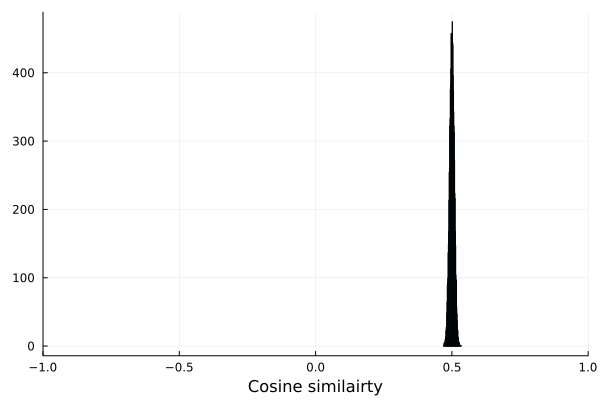
\includegraphics[scale = 0.7]{showcase}
    \caption{10000 cases of random 10000-dimensional bipolar vectors are made and each time implemented following example~\ref{eqn:ex1}. The resulting cosine similarities between $A$ and $A'$ are then plotted in a histogram.}
    \label{fig:exm1}
\end{figure}

We see that we can retrieve a lot of information with most of the cosine similarities centering around 0.5. Notice that two completely random HDVs would have a cosine similarity close to 0 just by stochastics. This result is not comparable to state-of-the-art accuracies but very efficient nonetheless as all of these calculations were done in less than 2 seconds. This same experiment was done with random binary 10000-dimensional vectors and it finished even faster as expected but retained the accuracy (similar \textit{Hamming distance} peak around 0.25).
\chapter[Hyperdimensional computing]{Hyperdimensional Computing}
Hyperdimensional computing (HDC) is a relatively recent paradigm of computing in which data is represented and manipulated by high-dimensional (or hyperdimensional) vectors in the range of tens of thousands bit. This framework, outlined by Kanerva~\cite{Kanerva2009}, is inspired by the workings of the human brain and its ability to adapt, learn fast and easily understand semantic relations. The human brain consists of about 100 billion neurons (nerve cells) and 1000 trillion synapses that connect these neurons. Each neuron is connected to up to 10,000 other neurons, creating massive circuits. This is likely fundamental to the workings of the human brain and what separates our brains from modern von Neumann computer architectures, which operate on 8 to 64-bit vectors. This becomes clear when we compare the relative simplicity for a human to learn a language compared to computers. Computers use a large and complicated set of arithmetic operations in the form of deep learning networks, which require terabytes of data and thousands of Watts of computing power to come close to mastering a language whilst a human can recognize other languages relatively easily when they don't even speak it. Likewise languages, we can very easily memorize and compare other intrinsically complex and contextual concepts such as images. A computer would have a hard time finding similarities between a set of images and faces because this requires very complex machine learning models. The human brain can do this all with a very large efficiency by consuming only roughly 20 W of energy.

Achieving these kinds of flexible brain-like models based on high dimensionality is not entirely new and is being explored since the 1990s. Some of these earlier models include Holographic Reduced Representations~\cite{HRR}, Spatter Code~\cite{spatter} and others. A hyperdimensional vector (HDV) can represent anything from a scalar number to any kind of concept. This vector is initially made up of totally random elements, but with a simple set of operations, which will be explained later, we can use other vectors to combine some concepts into new similar or dissimilar concepts. For example, to show the essence of HDC and how it tries to simulate the brain, we can compare the concept of a \textit{table} to the concept of a \textit{brocolli}. We would not immediately conclude that they are in any way similar but as humans, we can trace back \textit{table} to \textit{plate}, which has some similarities with \textit{food} from which we can easily extract the concept of \textit{brocolli} as in equation \ref{eqn:sem}. These kinds of operations are not very obvious for a classical computer but creating these semantic pathways and recognizing links between distant objects are rather easy for humans. Two unrelated concepts are noted by $\neq$ and two related concepts by $\approx$.
\begin{align}\label{eqn:sem}
    \begin{split}
    &\textrm{table} \neq \textrm{brocolli} \\        
    &\textrm{table} \approx \textrm{plate} \approx \textrm{food} \approx \textrm{brocolli}
    \end{split}
\end{align}
The elements in an HDV can be made up of binary bits (values from the set {0, 1}) like in classical computing but also of bipolar (values from the set {-1, 1}) or real numbers. The choice of the nature of the elements has also implications on the nature of the different operations and possibly the results.

An initial HDV is generated randomly. This \textit{holistic} or \textit{holographic} representation of a concept spread out over a vector consisting of thousands of bits gives rise to interesting properties such as its robustness agaisnt noise~\cite{hdctheo}. These kinds of systems are very tolerant to noise and failure of bits since we introduce a lot of redundancy in the vector just by stochastics. This is very unlike classical computing where every bit counts and one failure in a bit can lead to immediate data corruption. Besides its robustness, it also has the potential to perform much faster and more efficient computations than traditional computer systems since it allows for more efficient data storage by encoding multiple objects into a vector~\cite{Kanerva2009}\cite{hdctheo}.
\section{Operations on hyperdimensional vectors}
The interesting properties of HDC are based on only four basic operations we can perform on HDVs. We will discuss these for bipolar and binary vectors. From here, all implementations are written in the programming language Julia~\cite{Julia} unless noted otherwise. Known for its efficiency, Julia's blend of high-level, interpreter-based features makes it possible to write powerful programs. This is particularly beneficial when working with high-dimensional spaces. Julia's built-in support for bitvectors and bitmatrices, along with parallel computing, will be useful for this thesis. Furthermore, the lively Julia community supports a rich ecosystem and a broad array of packages to utilize.

Before the operations are demonstrated, we show how a random hyperdimensional vector can be generated in Julia. In the following code block, functions to generate binary and vectors can be made effortlessly with one line each.

\begin{minted}{julia}
# Built-in package for random number generation
using Random

# Binary HDV
bithdv(N::Int=10_000) = bitrand(N) 
#Bipolar HDV
hdv(N::Int=10_000) = rand((-1,1), N)
\end{minted}

\subsection*{Bundling} \label{sssec:add}
Also referred to as \textit{superposition} or \textit{aggregation}, the element-wise addition as in equation~\ref{eqn:sum} of $n$ input vectors $[X_{1} + X_{2} + \cdots + X_{n}]$ creates a vector $X$ that is similar to the input vectors.
\begin{equation}
    \label{eqn:sum}
    X = [X_{1} + X_{2} + \cdots + X_{n}]
\end{equation}
For bipolar vectors, this entails a straightforward element-wise addition. The resulting vector is restricted to a bipolar nature too depending on the sign of each element, thus containing only $-1$, $1$ but allowing $0$ for elements that are in disagreement as shown in the following $6$-dimensional example.
\begin{alignat*}{7}
    X_{1} &= && \qquad +1 && \qquad -1 && \qquad +1 && \qquad +1 && \qquad -1 && \qquad -1 \\
    X_{2} &= && \qquad +1 && \qquad +1 && \qquad +1 && \qquad -1 && \qquad -1 && \qquad -1 \\
    X_{3} &= && \qquad -1 && \qquad -1 && \qquad +1 && \qquad +1 && \qquad -1 && \qquad +1 \\
    X_{4} &= && \qquad -1 && \qquad -1 && \qquad -1 && \qquad +1 && \qquad -1 && \qquad +1 \\
    \hline
    [X_{1} + X_{2} + X_{3} + X_{4}] &= && \qquad \phantom{-}0 && \qquad -1 && \qquad +1 && \qquad +1 && \qquad -1 && \qquad \phantom{-}0
\end{alignat*}

For binary vectors, the vectors are element-wise bundled based on the majority element. This is no problem if an odd number of input vectors are considered but ambiguity rises when bundling an even set of vectors. This can be solved by setting the element in question randomly.~\cite{binBund} Another possibility is to add another random vector however this may seem to add more unnecessary noise, especially when bundling a low number of vectors. We can also reverse this by an \textit{inverse addition}. For bipolar vectors, this means just multiplying the vector of interest by -1. A binary vector can be flipped bit-wise. These kinds of operations are not directly built into Julia, but are easily programmed as followed:

\begin{minted}{julia}
# Adds bitvectors element-wise based on the majority element.
# Random if tied.
# Reduce function takes another function (here .+)
# and applies it to all given vectors.
# 'Dotted' operations such as .+ are vectorized
# making it element-wise.
function bitadd(vectors::BitVector ...)
    v = reduce(.+, vectors)            
    n = length(vectors) / 2
    x = [i > n ? 1 : i < n ? 0 : rand(Bool) for i in v]
    return x
end

# Adds bipolar vectors element-wise and rounds off to -1,0 or 1
# depending on the resulting sign.
add(vectors...) = reduce(.+, vectors) .|> sign
\end{minted}
Similar to an ordinary arithmetic summation, the bundling addition of hyperdimensional vectors is commutative so the result is not dependent on the order of addition.
\begin{equation}
    \label{eqn:sumcom}
    [X_{1} + X_{2}] = X = [X_{2} + X_{1}]
\end{equation}
\subsection*{Binding} \label{sssec:mult}
Two vectors can be multiplied element-wise resulting in a vector maximally dissimilar to the input vectors. Vectors $X$ and $Y$ are bound together forming $Z$ being orthogonal to $X$ and $Y$ as shown in equation~\ref{eqn:multp}.
\begin{equation}
    \label{eqn:multp}
    Z = X \circ Y
\end{equation}
This \textit{binding} operation translates to a simple arithmetic element-wise multiplication for bipolar vectors. For binary vectors, this is represented by a \textit{XOR} bit-operation shown as follows.
\begin{alignat*}{7}
    X &= && \qquad 1 && \qquad 0 && \qquad 1 && \qquad 1 && \qquad 0 && \qquad 0 \\
    Y &= && \qquad 1 && \qquad 1 && \qquad 0 && \qquad 1 && \qquad 0 && \qquad 1 \\
    \hline
    X \circ Y &= && \qquad 0 && \qquad 1 && \qquad 1 &&  \qquad 0 && \qquad 0 && \qquad 1
\end{alignat*}
In Julia, there is a built-in function to carry out bit-operations such as \textit{XOR}. For bipolar vectors, a simple element-wise multiplication suffices.

\begin{minted}{julia}
# Bind binary vectors
bitbind(vectors::BitVector ...) =  reduce(.xor, vectors)

# Bind bipolar vectors
bind(vectors...) = reduce(.*, vectors)
\end{minted}

The binding operation can also be undone by multiplying with the same vector again. It is its own inverse so that:
\begin{equation}
    \label{eqn:multpinv}
    A \circ A = O
\end{equation}
Where $O$ is a vector containing only zeros. Likewise an ordinary multiplication, this operation is commutative and distributive over additions, meaning that transforming a bundle of concepts with binding is equivalent to binding every element before bundling.
\begin{equation}
    \label{eqn:multpdis}
    A = Z \circ (X + Y) = X \circ Z + Y \circ\ Z
\end{equation}
\subsection*{Permutation} \label{sssec:perm}
The permutation operation of an HDV, is a reordering of the contents of the HDV. This can be random but a circular shift is widely employed~\cite{HD_rev} and makes the operation easily reversible. This results in a vector technically dissimilar from the input vector but still encoding its information. This will become important later when it will be used to encode sequential information such as tokens in a text. This operation will be denoted by $\Pi$.
\begin{alignat*}{7}
    X &= && \qquad 1 && \qquad 0 && \qquad 1 && \qquad 1 && \qquad 0 && \qquad 0 \\
    \hline
    \Pi(X) &= && \qquad 0 && \qquad 1 && \qquad 0 &&  \qquad 1 && \qquad 1 && \qquad 0
\end{alignat*}
In Julia, this line can do it for both binary and bipolar vectors:

\begin{minted}{julia}
# Permute by applying a circular shift
perm(vector::AbstractVector, k::Int=1) = circshift(vector, k)
\end{minted}

\subsection*{Similarity measurement} \label{sssec:sim}
For many kinds of problems, it will be necessary to quantify the similarity between two HDVs. The method depends on the nature of the vectors. For binary vectors, the \textit{Hamming distance} defined as:

\begin{equation}
    \label{eqn:Hamming}
    \text{Ham}(A, B) = \frac{1}{d} \sum_{i=1}^{d} 1_{A_{(i)} \neq B_{(i)}}
\end{equation}
The \textit{cosine distance} as defined in equation~\ref{eqn:cosine} is most commonly used for bipolar vectors:
\begin{equation}
    \label{eqn:cosine}
    cos(A, B) = \frac{A \cdot B}{||A|| * ||B||}
\end{equation}
Both are not built-in Julia by default, but can be programmed as followed:
\begin{minted}{julia}
# Built-in package for linear algebra operations 
using LinearAlgebra

# Hamming distance
hamming(x::BitVector, y::BitVector) = sum(x .!= y)/length(x)

# Cosine similarity
cosine(x::Vector, y::Vector) = dot(x, y) / (norm(x) * norm(y))
\end{minted}
The results of both of these measurements are summarized in table~\ref{tab:dist}.
\begin{table}[h]
    \centering
    \caption{\label{tab:dist}Overview of similarity measurements in HDC depending on the nature of the HDVs}
    \begin{tabular}{|cccc|}
        \hline
        \textbf{Measurement} & \textbf{Dissimilar} & \textbf{Orthogonal} & \textbf{Similar} \\
        \hline
        \textbf{Hamming distance} & 1 & 0.5 & 0 \\
        \hline
        \textbf{Cosine similarity} & -1 & 0 & 1 \\
        \hline
    \end{tabular} 
\end{table}

It is important to note that two random HDVs will be quasi-orthogonal to each other just by stochastics. Also notice that the first quantifies a distance and the latter a similarity.
\section{Examples}
There are many interesting possibilities given the relative simplicity of all these operations. In this section, we will demonstrate the power of hyperdimensional computing with some simple examples.
\subsection*{Simple example with simulated data}
To get a feel for the operations, assume $A, B, C, X, Y$ and $Z$ to be random 10,000-dimensional bipolar hypervectors and that $D = X \circ A + Y \circ B + Z \circ C$, let us then try to retrieve A from D by using the defined operations. We generate for $A, B, C, X, Y$ and $Z$ each a random 10,000-D vector. To retrieve an approximation of A, D can be multiplied by X and the rest of the included vectors are then regarded as noise as done in equations~\ref{eqn:ex1}. Because of the robustness of hyperdimensional vectors, a lot of information of A should still be contained within D.
\begin{align}\label{eqn:ex1}
\begin{split}
    A' &= X \circ D \\
    &= X \circ (X \circ A + Y \circ B + Z \circ C) \\
    &= \underbrace{X \circ X \circ A}_A + \underbrace{X \circ Y \circ B + X \circ Z \circ C}_\text{noise} \\
    &\approx A
\end{split}
\end{align}
 The procedure of equation~\ref{eqn:ex1} is repeated 10,000 times because of the stochastic nature of these vectors. The results are illustrated in figure~\ref{fig:exm1}.
\begin{figure}[h]
    \centering
    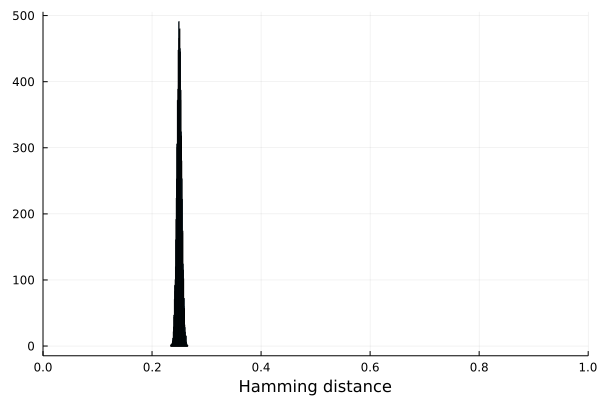
\includegraphics[scale = 0.2]{output.png}
    \caption{10,000 cases of random 10,000-dimensional binary vectors being made by equation~\ref{eqn:ex1}. The resulting Hamming distances between $A$ and $A'$ are then plotted in a histogram. Dashed line indicates a Hamming distance of 0.5, meaning that two vectors are orthogonal.}
    \label{fig:exm1}
\end{figure}
We see that we can retrieve a lot of information with most of the Hamming distances centering around 0.25. Due to the high-dimensional space and thus its robustness, the distances are very consistent. Notice that two completely random HDVs would have a distance close to 1 just by stochastics. A Hamming distance of 0 would mean that we retrieved all bits of A correctly, which is impossible in this model due to the consideration of noise. Although we work with a very constrained model, vector A is roughly 75 \% retrievable and the calculations are very efficient as all of these can be completed in less than 2 seconds on a laptop. This same experiment was done with random bipolar, 10,000-dimensional vectors and it performs slightly slower as expected but retained the accuracy.
\section{Examples of hyperdimensional computing with real datasets}
\label{sec:example}
Now, the power of these simple operations will be demonstrated by applying them to a couple of relatively small real datasets.
\subsection*{Zoo animal classification}
As the first example, we will consider a simple dataset containing 101 animals with 17 descriptors such as their number of legs, their skin covering and other physical properties~\cite{zoo}. Our goal is to create a simple model that can classify these animals and other animals that are not present in the dataset based on their descricptors. To tackle this problem, we first assign to each descriptor a random hyperdimensional vector. For each animal, all of its features can be bundled to obtain a final vector representing the animal. For example, it is known that a chicken lays eggs, is covered with feathers and has two legs so then these features can be bundled as in the following equation. $C$ is a vector representing a chicken, $E$ the ability to lay eggs, $F$ the possession of feathers and $T$ the possession two legs:
\begin{equation}\label{eqn:chicken}
    C = E + F + T
\end{equation}
This is simple for all the variables that have binary values, but the feature for the number of legs is variable. Although it is possible to assign completely random vectors to each number of legs, it would make a slightly more biologically realistic model if an animal with 2 legs would be more similar to one with 4 legs than to one with 8 legs. To address this, a range of numbers would have to be representable by hyperdimensional vectors, the range from 0 to 8 in this case. First, a random hyperdimensional vector representing the lower bound of the interval is generated. Next, a vector representing the next step in the interval is constructed by replacing a fraction of the vector with random bits. This last step is then repeated to obtain a vector of each number in a range.

In biology, it is possible to find higher-order of concepts that are combinations of directly observable characteristics. For example, an animal could lay eggs or be dependent on its mother's milk, but (almost) never both. So, the growth and development of an animal depend on these characteristics. This property can be easily implemented into this HDC model by binding an HDV of a higher order concept to the descriptor HDV. So as said previously, the 'milk' ($M$), and 'egg' ($E$) features yields information about the growth of the animal, so we will create another vector representing the growth feature ($G$) to obtain a more expanded model. This is also done for the skin protection features ($S$) and all the features considering the limbs ($L$). This also gives us the possibility to retrieve some features of the animals as in the procedure shown in the previous example. Thus, equation~\ref{eqn:chicken} can be expanded into:
\begin{equation}
    C = G \circ E + S \circ F + L \circ T
\end{equation}

After conducting the various procedures, the data set now consists of 101 animals, each represented by a 10,000-dimensional feature vector. To efficiently analyze and visualize this high-dimensional data, principal component analysis (PCA) has been employed to reduce the dimensionality from 10,000 to just two. By projecting these vectors onto a 2D space, the data can be conveniently displayed in a two-dimensional plot, as illustrated in Figure \ref{fig:exm2}. Upon examination of the plot, three distinct and meaningful clusters of animal classes emerge, which align well with our understanding of evolutionary relationships. These clusters include: (1) mammals, (2) a group consisting of birds, reptiles, and amphibians, and (3) a cluster encompassing invertebrates and insects. While the current analysis already provides valuable insights into the relationships between different animal classes, further improvement could be achieved by incorporating additional features that may lead to a clearer separation of these groups. By doing so, the model would be able to more accurately distinguish between the different animal classes and provide a more comprehensive understanding of their evolutionary connections.
\begin{figure}[h]
    \centering
    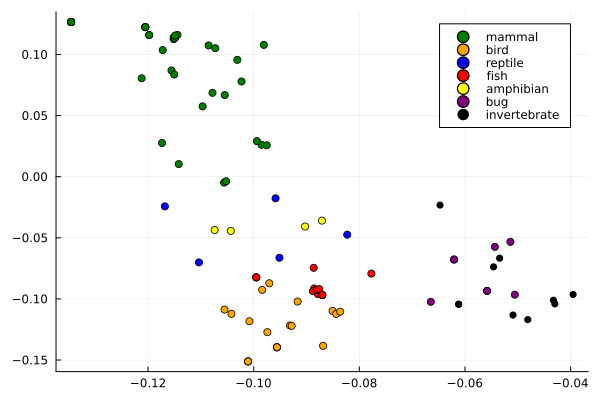
\includegraphics[scale = 0.5]{pca1.png}
    \caption{Scatter-plot of the first two principal components (PCs) of a 101$\times$10,000 matrix containing hyperdimensional vectors for every animal in the zoo dataset after a PCA procedure. These PCs account for roughly 48 \% of the variance.}
    \label{fig:exm2}
\end{figure}

After an HDV has been made for every animal, all animals of the same class can be bundled to obtain an HDV representing the said class. So for example, if we have a hyperdimensional vector for a pigeon ($P$), chicken ($C$) and a kiwi ($K$), an HDV representing birds ($B$) can be made by doing:
\begin{equation}
    B = [P + C + K]
\end{equation} 
To classify an animal, its HDV can be compared to the HDVs of every class and the most similar vector is then assumed to be its class.  In the following code block, the hypervectors for every animal and class have been already made as discussed above. The resulting HDV for a flamingo has been compared to every other class vector \textit{via} a measurement of the Hamming distance. The distance of flamingo HDV to the bird HDV is significantly smaller than to all other vectors
\begin{figure}[H]
    \centering
\begin{minted}{julia}
# HDVs for every animal class HDVs have been made already
# Take flamingo HDV out of dataframe
flamingo = data.species_hdv[24]
println("Hamming distance to mammal = ",
hamming(flamingo, mammal))

println("Hamming distance to bird = ",
hamming(flamingo, bird))

println("Hamming distance to reptile = ",
hamming(flamingo, reptile))

println("Hamming distance to amphibian = ",
hamming(flamingo, amphibian))

println("Hamming distance to bug = ",
hamming(flamingo, bug))

println("Hamming distance to fish = ",
hamming(flamingo, fish))

println("Hamming distance to invertebrate = ",
hamming(flamingo, invertebrate))

# Output
# Hamming distance to mammal = 0.303
# Hamming distance to bird = 0.1044
# Hamming distance to reptile = 0.2727
# Hamming distance to amphibian = 0.313
# Hamming distance to bug = 0.2867
# Hamming distance to fish = 0.3484
# Hamming distance to invertebrate = 0.4061
\end{minted}
\end{figure}
For further improvement, it would be possible to generate a set of animals not present in the dataset and test those in order to further understand how this model can be improved. On top of this, it would also be possible to generate a confusion matrix to understand where we could use more distinguishing descriptors. From the PCA, we could already predict that reptiles and amphibians would be easily confused, as for invertebrates and bugs.
\subsection*{Protein classification}
\label{ssec:protclas}
To illustrate an example more akin to this research topic, a model based on the principles of hyperdimensional computing will be built to classify a protein sequence dataset~\cite{anticancer}. It contains 949 manually curated peptide sequences with their membranolytic anti-breast cancer activity level (very active, moderately active, experimentally inactive and virtually inactive). The virtually inactive peptides are predicted to be inactive. The model will be built with mostly the same procedure as for the animal classifier, but instead of animals, sequences have to be encoded into HDVs now. First, a random HDV is generated for every amino acid. Physicochemical properties, evolutionary constraints etc. could be introduced to make this model more realistic but that is not necessary for this demonstration. Next, a peptide sequence is to be considered as a bag of trimers as seen in figure~\ref{fig:diagram_exprot5}. A vector representing a trimer is generated by binding the three amino acids whilst retaining sequential information by shifting as in equation~\ref{eqn:trimer}. All retrievable trimers from a given sequence are then bundled together, forming a vector representative of the sequence. 
\begin{equation}\label{eqn:trimer}
    ABC = A \circ \Pi (B) \circ \Pi (\Pi (C))
\end{equation}
\begin{figure}[h]
    \centering
    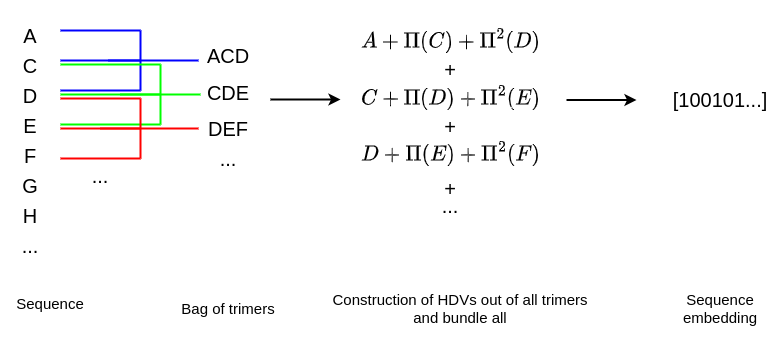
\includegraphics[scale = 0.55]{diagram_exprot.png}
    \caption{Overview of operations done to obtain an HDV of a protein sequence for the example concerning the real peptide dataset. First, a random HDV is generated for every amino acid. Next, a peptide sequence is to be considered as a bag of trimers. A vector representing a trimer is generated by binding the three amino acids whilst retaining sequential information by shifting as in equation~\ref{eqn:trimer}. All retrievable trimers from a given sequence are then bundled together, forming a hyperdimensional vector representation of the sequence.}
    \label{fig:diagram_exprot5}
\end{figure}
From here on, the same procedures as in the last example can be applied here too, so all HDVs of a class are bundled for further analysis. The PCA procedure did not generate interesting results because the two first principal components explained only 5 \% of the variance. This means that it is not feasible to reduce the 10,000 dimensions of the vectors to two, likely because the information is too smeared out over the vectors. This occurrence is highly dependent on the training data. Nevertheless, this follows the philosophy of hyperdimensional computing in keeping holistic representations of concepts.

\begin{figure}[H]
    \centering
    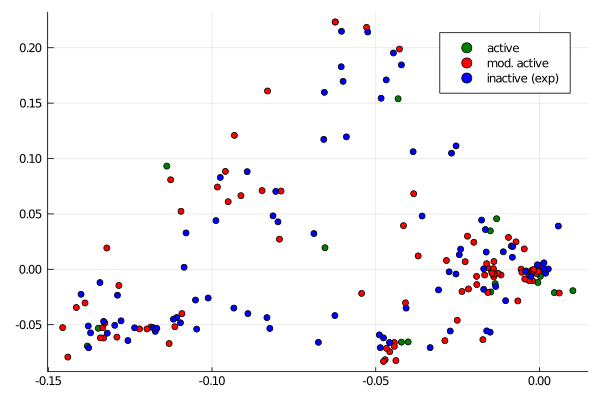
\includegraphics[scale = 0.5]{exampprot.png}
    \caption{Scatter-plot of the first two principal components, projecting the 10,000-dimensional vectors for every peptide into the 2 main PCs. These PCs account for roughly 5 \% of the total variance}
    \label{fig:diagram_exprot}
\end{figure}

Next, a classifier was made correspondingly. The dataset was stratified and split into a training set (comprising 80 \% of the sequences) and a test set. With 100 runs, it could predict a protein sequence's class with an accuracy of 85 \%. It has to be taken into account that the predicted inactive peptides account for 80 \% of the sequences of the dataset, thus this model performs slightly better than if we would predict at random. There are many possible improvements to be made however, such as using more suitable performance metrics, introducing similarities between amino acids instead of setting them randomly and using more suitable frameworks for our protein classification models, which will all be research topics further on in this project.
\chapter[Amino acid and protein encoding]{Hyperdimensional computing methods to encode amino acids and protein sequences}
\section{Introduction}
To research the possibilities of the hyperdimensional computing framework applied to protein language modeling, we introduce a rudimentary pipeline. First, amino acids would have to be encoded into hyperdimensional vectors. These vectors for every separate amino acid could be then further encoded into vectors representing a full protein. And lastly, these embeddings could be then utilized to perform predictions such as classifications as shown in figure~\ref{fig:pipeline}. The first two steps of this pipeline will be discussed further in this chapter.

\begin{figure}[H]
    \centering
    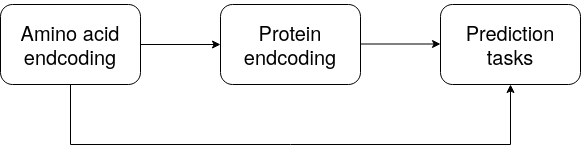
\includegraphics[scale = 0.5]{pipeline}
    \caption{A simple demonstration of our workflow. First, we encode single amino acids into hyperdimensional vectors. With these, protein sequences could be encoded into hyperdimensional vectors. Lastly, both kinds of embeddings are then used for prediction tasks.}\label{fig:pipeline}
\end{figure}

\section{Encoding single amino acids into hyperdimensional vectors}
Currently, in most of the research in hyperdimensional computing, there is an emphasis on creating and assigning hyperdimensional vectors to certain concepts at random. This is useful for optimizing speed and efficiency and is not a problem for many prevalent research areas such as natural language processing, where, for example, it is typically assumed that a letter's similarity to other letters in the alphabet remains constant. However, hyperdimensional computing sees minimal application in the context of biological data. Some notable studies include HDNA which assigns random hyperdimensional vectors to DNA bases to encode DNA sequences and BioHD~\cite{biohd} which encodes protein sequences using random mRNA hypervectors to use in genome sequence searches. In the context of DNA sequencing, the assumption of assigning random hyperdimensional vectors may not present as significant an issue as with proteins. This is largely due to the distinct nature of DNA bases as they do not display the same degree of physicochemical diversity that amino acids in proteins do. DNA bases serve primarily as the information carrier in the biological system, with their sequence dictating the sequence of amino acids in proteins. In this role, the relevance of their physicochemical properties to their informational role is rather limited in comparison to amino acids, which main function is to dictate the structure and function of the resulting protein. Whilst there are phenomena in DNA structures such as base stacking and hydrogen bonding that play a role, the simple base-to-vector mapping often suffices.

When considering protein language modeling, however, this assumption might be suboptimal since some amino acids are chemically more similar to each other than to others which is crucial to the protein's structure and function. We can already estimate physicochemical distances between amino acids based on their physicochemical properties~\cite{physicochem} such as volume, polarity, chemical groups etc. \textit{via} many kinds of distance measures. The different similarities between amino acids are tied into the structure and thus function of amino acid sequences and shape our view of protein language. It explains why some amino acid substitutions can result in almost no phenotypical changes or on the other hand detrimental changes. Proteins have evolved to maintain their structure and function, and drastic changes in physicochemical properties can disrupt these characteristics. Therefore, amino acid substitutions that preserve the physicochemical properties of the original amino acid are more likely to be selected, resulting in a negative correlation with physicochemical distance. To account for this, we experimented with several methods to encode physicochemical distance into amino acid hypervectors.

Besides encoding amino acids as building blocks, it is also useful to encode amino acids in the context they are found in. State-of-the-art protein language models have the ability to gather information on long-range dependencies around a single amino acid and encode this information into neural networks and in dense numerical vectors. These models are very powerful, but as discussed earlier very resource-intensive too. To investigate the possibilities of developing contextual embeddings on the level of amino acids, we propose a novel encoding technique within the hyperdimensional computing framework.

\section{Encoding proteins into hyperdimensional vectors}
In section~\ref{ssec:protclas}, we introduced the bag-of-words (BoW) method of embedding sequences in hyperdimensional space which has been extensively applied to cases related to natural language processing in a hyperdimensional computing context. We also introduce a novel sequence embedding method in hyperdimensional computing.

\section{Methods}
From here on, every hyperdimensional vector is made to be 10,000-dimensional and binary unless noted otherwise. 
\subsection*{Encoding single amino acids into hyperdimensional vectors}
\subsubsection*{Projected ESM-2 embeddings}
The last layer of the 3 billion-parameter ESM-2 model~\cite{esm2} of every amino acid was extracted, resulting in 1024-dimensional real-valued embeddings for every amino acid. To project these into hyperdimensionality, a simple matrix multiplication has been employed: 
\[A_{1x1024} \times B_{1024x10,000} = C_{1x10,000}\]
Where $A$ is a 1024-dimensional ESM-2 embedding and B a matrix of 1024 random 10,000-D vectors. The resulting vectors are then min-max scaled and rounded depending on the desired nature of the vectors. To visually assess these, the vectors for each amino acid are reduced in dimensionality \textit{via} PCA into 2 dimensions. This has been compared to a PCA of the unaltered 1024-dimensional ESM-2 embeddings.
\subsubsection*{Real-valued projected ESM-2 embeddings}
It is possible to step away from binary hyperdimensional vectors, which are typically used in hyperdimensional computing research, and allow the vectors to be real-valued. This gives us the possibility to store more data in a vector and utilize more complex mathematical operations with the cost of losing efficiency of bit-operations. We generated random real-valued vectors with random values in [-1,1]. Real-valued ESM-2 embeddings were generated by the same procedure as above, but without the rounding.
\subsubsection*{Enforcing similarities using genetic algorthims}
Instead of utilizing embeddings coming from other large protein language models, we also experimented with encoding predetermined target pairwise distances onto initially random hyperdimensional vectors. First, a suitable matrix with predetermined pairwise distances has to be considered. This also implies that the matrix has to be symmetric. If we then consider the 20 essential amino acids, the problem at hand would involve a set of 20 binary vectors of length 10,000 to conform to a target distance matrix based on Hamming distance. This can be classified as a combinatorial optimization problem as it involves searching for an optimal or near-optimal configuration of binary vectors that satisfy a specific criterion. To minimize the difference between the target and actual Hamming distances for all pairs of binary vectors, we could adjust the vectors by randomly bit-flipping them until they meet the desired criteria. However, the search space in this problem is vast ($2^{10,000 x 20}$), making exhaustive search methods computationally infeasible. Thus, more efficient algorithms are needed to solve this problem such as genetic algorithms~\cite{GA} (GAs). GAs, a subfield of evolutionary algorithms, draw inspiration from the process of natural selection and emulate the evolutionary mechanisms of crossover, mutation, and selection to explore a vast search space and converge toward an optimal or near-optimal solution. A genetic algorithm was implemented with the \textit{Evolutionary.jl v0.11.1}~\cite{evojl} package in \textit{Julia} to encode target similarities. The primary steps of a genetic algorithm include:
\begin{itemize}
    \item Initialization: random candidate solutions are initiated with a given population size.
    \item Crossover: combine genetic material offspring of two parents (in this case vectors). There are many recombination techniques such as single-point, multi-point and uniform crossover.
    \item Mutation: randomly alterate genes (in this case bits) to explore other possibilities of configurations and prevent premature convergence due to local optima.
    \item Evaluation: Each individual in the population (in this case a set of vectors) is assessed using a fitness function, which measures how well the solution solves the given problem.
    \item Selection: individuals from the population are selected based on their fitness to create a mating pool. Fitter individuals have a higher probability of being selected, mimicking the concept of survival of the fittest in natural evolution.
\end{itemize}
These steps are reiterated over a number of generations to obtain a set of vectors that correspond to the best fitness. A \textit{BLOSUM62} substitution matrix \cite{blosum} and Grantham's distance matrix \cite{aa_evolution} were considered as target pairwise similarity matrices for the GA. These were then normalized to obtain the target pairwise Hamming distances. The fitness is determined by the sum of the squared differences between the computed distance matrix of an individual and the target distance matrix. The lower the fitness value, the more optimal the individual. The population size was set to 25000 and the number of generations to 250. The mutation rate was set to 0.15 and the crossover rate to 0.2, these are high and low respectively compared to more commonly used parameters because we want to emphasize the bit-flipping and avoid recombination of vectors for faster convergence.
\subsubsection*{Contextualized neighborhood-encoding of amino acids}\label{sssec:trans}
To encode the neighborhood of an amino acid in a sequence, all possible pairwise interactions with the central amino acid in question in a given window are made \textit{via} binding and then all encoded into one vector \textit{via} bundling as shown figure~\ref{fig:AAtr}. Our neighborhood-encoder was tested on the human reference proteome in UniProt, entry \textit{UP000005640}, containing 20591 proteins. We started with real-valued random vectors and real-valued projected ESM-2 vectors for every amino acid. Windows of $n = 4$ and $k = 50$ were considered resulting in 4 different experiments. Every single residue in the human reference proteome was encoded with information within the k-range window and an average vector was made for every amino acid. For all 20591 peptides in the reference proteome, this procedure took only 3 hours for $n = 4$, but upwards to 15 hours for $n = 50$ on a high-performance computing cluster (HPC). After all amino acids were encoded, an element-wise average was made for every amino acid. The resulting hyperdimensional vectors were kept to a real-numbered nature to not lose information for illustrative purposes. Principal component analysis was then done for these 4 experiments as seen in figure~\ref{fig:bigfig}. 

\begin{figure}[H]
    \centering
    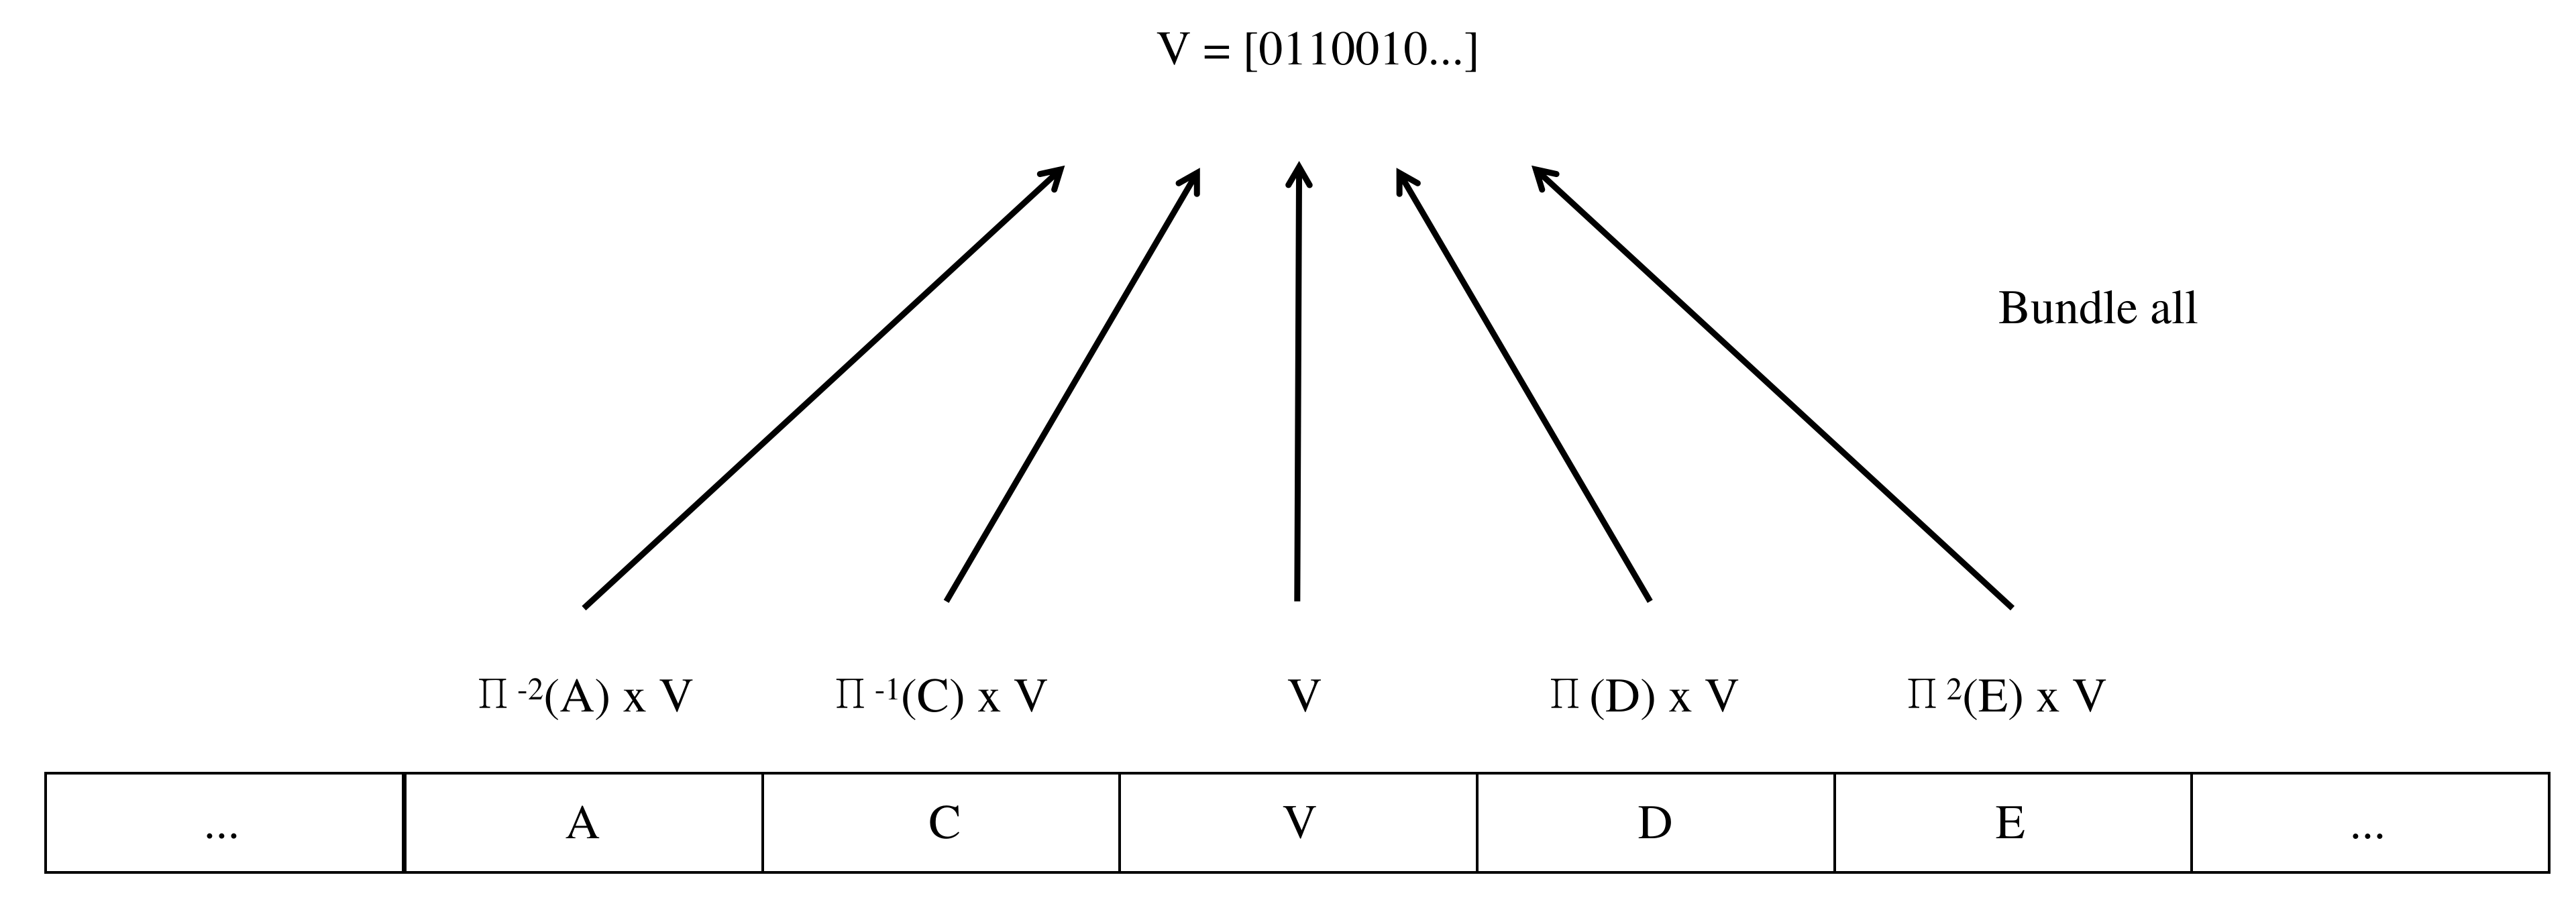
\includegraphics[scale = 0.43]{transformerlike}
    \caption{A simple demonstration of our amino acid encoder. First, HDVs are generated for every kind of amino acid, this can be done using just random HDVs, projected ESM-2 embeddings, GA-optimized vectors etc. It considers an amino acid and all amino acids in a predetermined neighborhood (here $n = 2$). It produces all possible interactions of the central amino acid in the window by binding and then bundles all the pairwise interactions into one hyperdimensional vector that represents the central amino acid.}\label{fig:AAtr}
\end{figure}

\subsection*{Encoding proteins into hyperdimensional vectors}\label{ssec:protseq}
We implemented two different algorithms to encode amino acid vectors into vectors representing proteins. We already introduced the BoW-method in section~\ref{ssec:protclas}, fully explained in figure~\ref{fig:diagram_exprot5}. We also introduce a novel sequence embedding method in hyperdimensional computing.  It is similar to the bag-of-words method in the sense that it bundles vectors of k-mers, but here, the k-mer's positional information will be encoded into the k-mer by permuting it before bundling as seen in figure~\ref{fig:cnn}, similarly to how a convolutional layer in a neural network operates so we will name it the convolutional embedding method from here on. These methods will be extensively utilized and tested in chapters 4 and 5 where several case studies consisting of protein sequences datasets are tackled.

\begin{figure}[h]
    \centering
    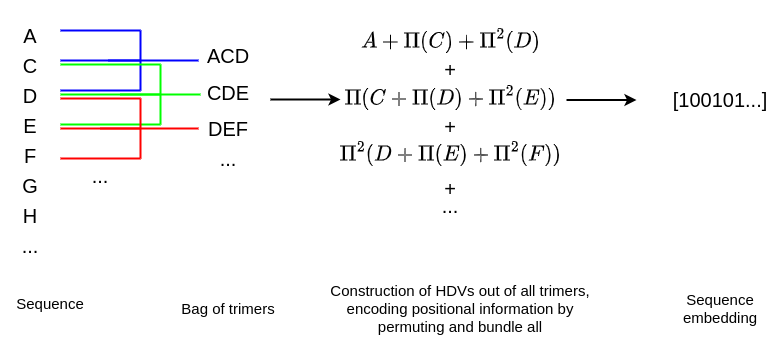
\includegraphics[scale = 0.6]{cnn.png}
    \caption{Overview of operations done to obtain an HDV from a sequence using the convolutional embedding method. First, an HDV is generated for every amino acid. Next, a peptide sequence is to be considered as a bag of trimers. A vector representing a trimer is generated by binding the three amino acids whilst retaining sequential information by shifting as in equation~\ref{eqn:trimer}, just as in the BoW-method (figure~\ref{fig:diagram_exprot}). On top of that, every trimer will also be positionally encoded via a permutation operation. All retrievable trimers from a given sequence are then bundled together, forming a hyperdimensional vector representative of the sequence.}\label{fig:cnn}
\end{figure}

\section{Results}
\subsection*{Projected ESM-2 embeddings}
Visually, no interesting patterns can be deducted from the PCA decompositions of the ESM-2 embeddings. Yet, if we also perform a principal component analysis on random vectors, we can see there is significantly more variance encoded into the first two principal components of the ESM embeddings (22 \%) compared to random vectors (10.5 \%, can deviate slightly depending on the run), meaning that there should be a significant amount of similarity encoded into the hyperdimensional vectors. PCA decomposition of our projected ESM-2 embeddings can't fully retrieve the variance in the hyperdimensional vectors as well as in the unaltered ESM-2 embeddings, as to be expected. The performance and usefulness may be shown more clearly when tested in other computational biology problem settings.

\begin{figure}[H]
\label{fig:combined_ESM_embeddings}
\centering
\begin{minipage}[b]{.5\textwidth}
    \begin{subfigure}[b]{\textwidth}
    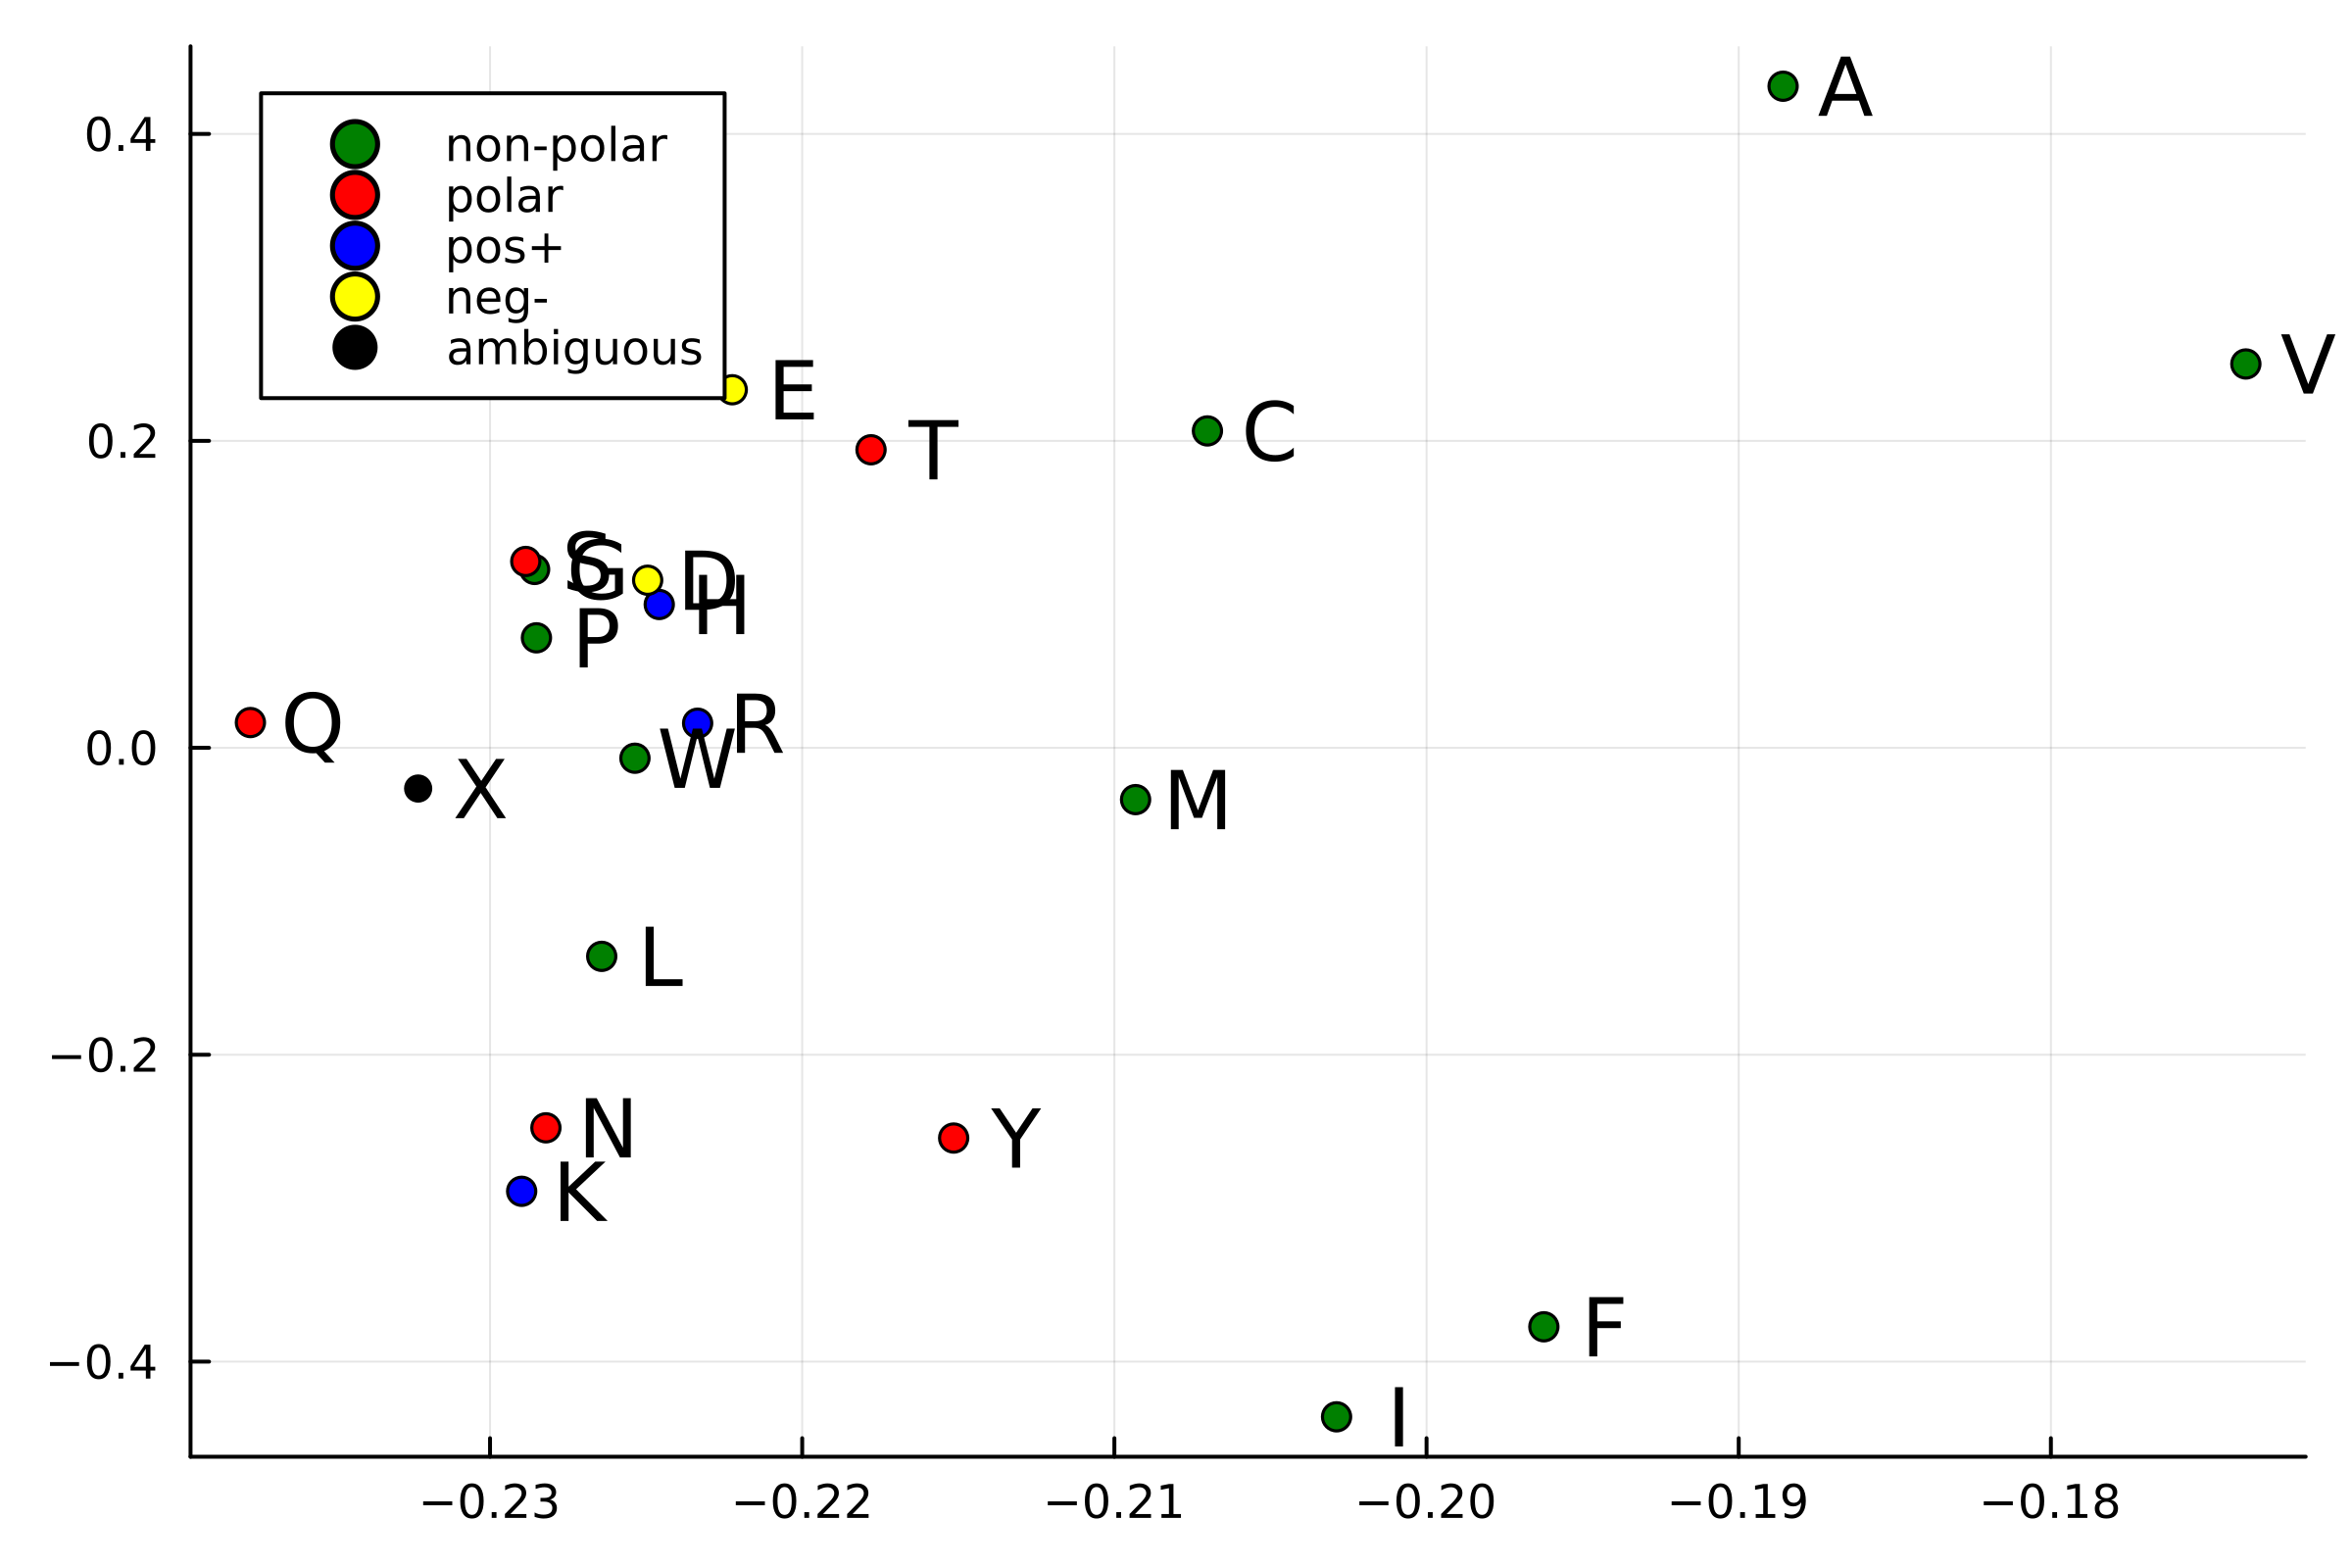
\includegraphics[width=\textwidth]{esm_emb_1028}
    \caption{Unaltered 1024-dimensional ESM-2 embeddings}
    \label{fig:AAesm_pure}
\end{subfigure}
\end{minipage}
\\
\centering
\begin{minipage}[b]{.5\textwidth}
\begin{subfigure}[b]{\textwidth}
    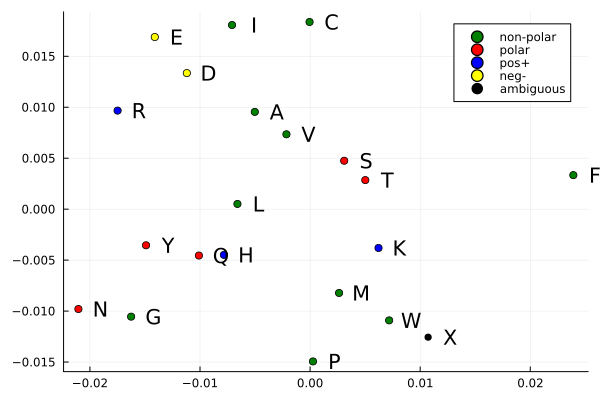
\includegraphics[width=\textwidth]{esm_emb}
    \caption{ESM-2 embeddings projected into binary hyperdimensionality}
    \label{fig:AAesm}
\end{subfigure}
\end{minipage}
\\
\centering
\begin{minipage}[b]{.5\textwidth}
\begin{subfigure}[b]{\textwidth}
    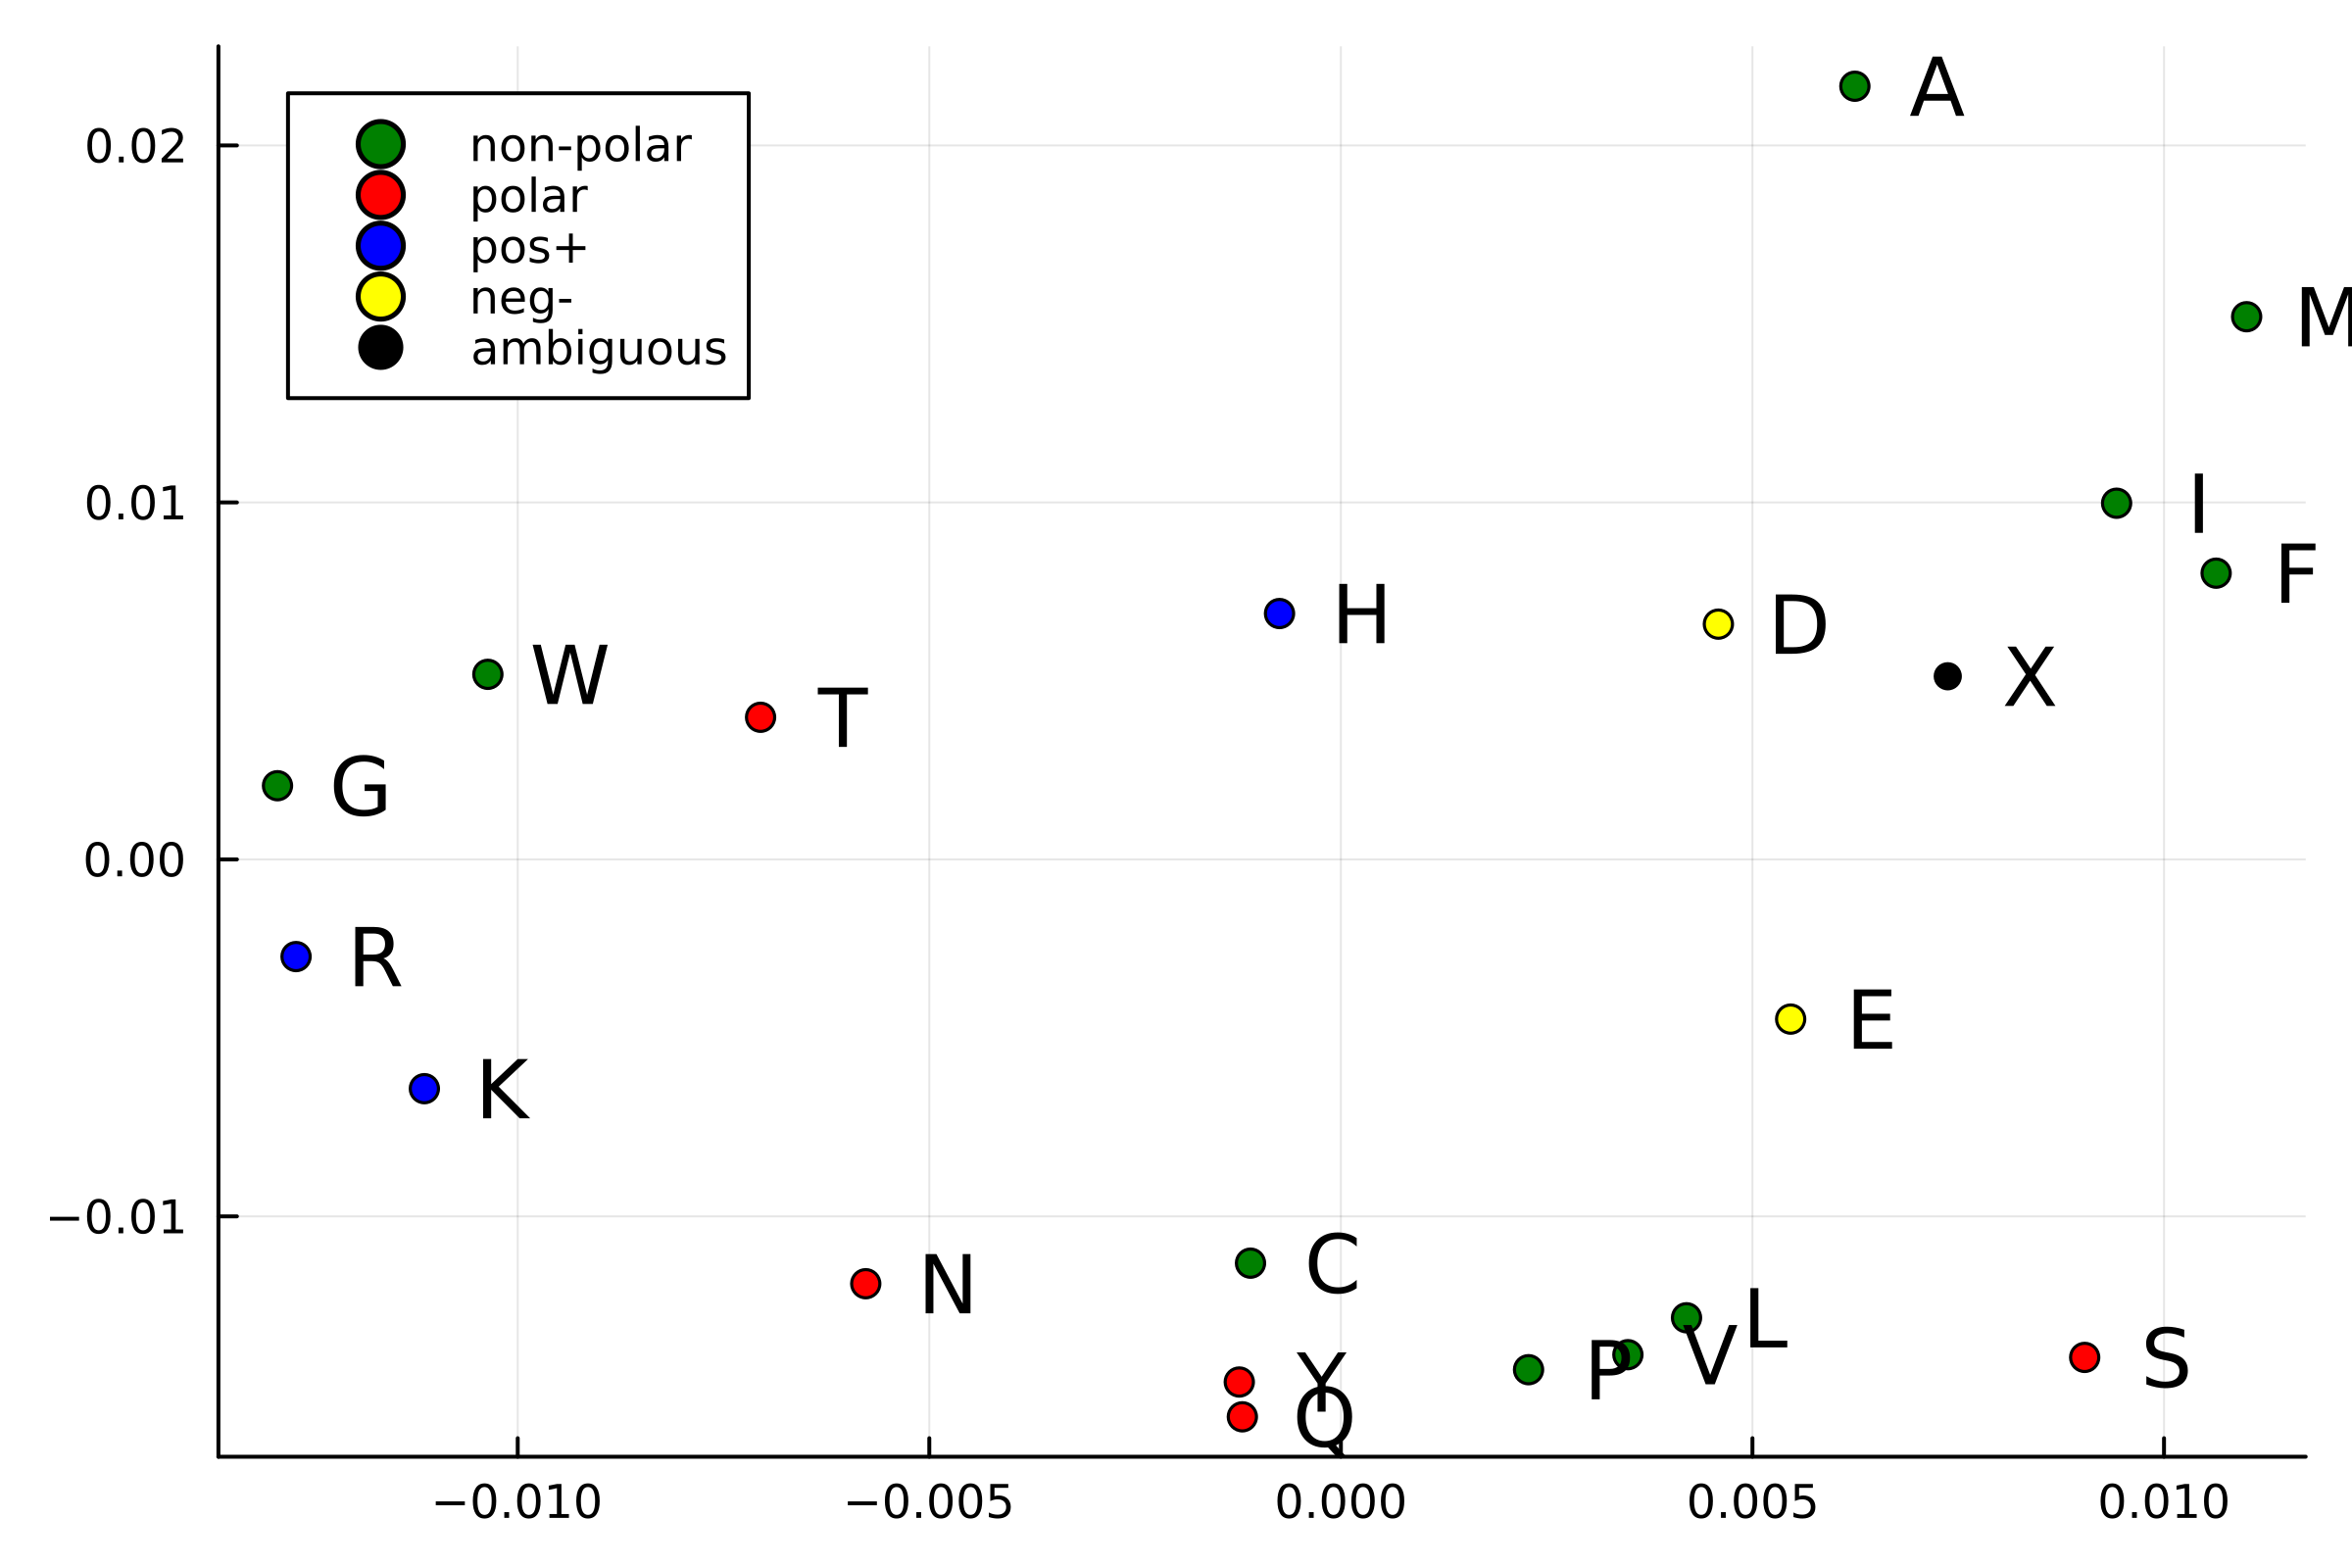
\includegraphics[width=\textwidth]{esm_emb_HDVreal}
    \caption{Real-value projected ESM-2 embeddings.}\label{fig:AAesmreal}
\end{subfigure}
\end{minipage}
\caption{Scatter-plots of the first two principal components of ESM-2 embeddings for amino acids. (a) Unaltered 1024-dimensional ESM-2 embeddings, accounting for roughly 79 \% of the total variance. (b) ESM-2 embeddings projected into hyperdimensionality, accounting for roughly 22 \% of the total variance. (c) real-valued projected ESM-2 embeddings, accounting for roughly 28.5 \%. In all subfigures, amino acids are annotated and colored based on their chemical property of polarity.}
\end{figure}

\subsection*{Real-valued projected ESM-2 embeddings}
The PCA of the real-valued projected ESM-2 vectors, as seen in figure~\ref{fig:AAesmreal}, appears to capture a greater proportion of the variance compared to their binary counterparts. This increased detected variance is likely attributed to the reduction in data loss that occurs when avoiding the rounding off of values. The effectiveness of these real-valued projected ESM-2 vectors in various tasks will be further investigated and evaluated in subsequent analyses.

\subsection*{Enforcing similarities using genetic algorthims}
The outcomes of employing a genetic algorithm to infer our target distances can be found in the tables located in section~\ref{app:chp3} of the appendices. These are visually presented as heatmaps in figure~\ref{fig:ga}. Taking into account that two random hyperdimensional vectors would be quasi-orthogonal just by stochastics, their Hamming distances would be close to 0.5. Hence, one could see that despite our efforts, our obtained distances remain significantly different from the desired values and still indicate quasi-orthogonality, which led us to discontinue further exploration of these vectors. This discrepancy is likely attributable to the vast search space associated with the problem, resulting in substantial computational time required to reach the target matrix. The optimization process ran for approximately 58 hours on a high-performance computing (HPC) system. Unfortunately, utilizing a genetic algorithm does not appear to be a viable method for optimizing our vectors within an acceptable timeframe.

\begin{figure}[H]
    \centering
    \begin{minipage}[b]{.5\textwidth}
    \begin{subfigure}[b]{\textwidth}
        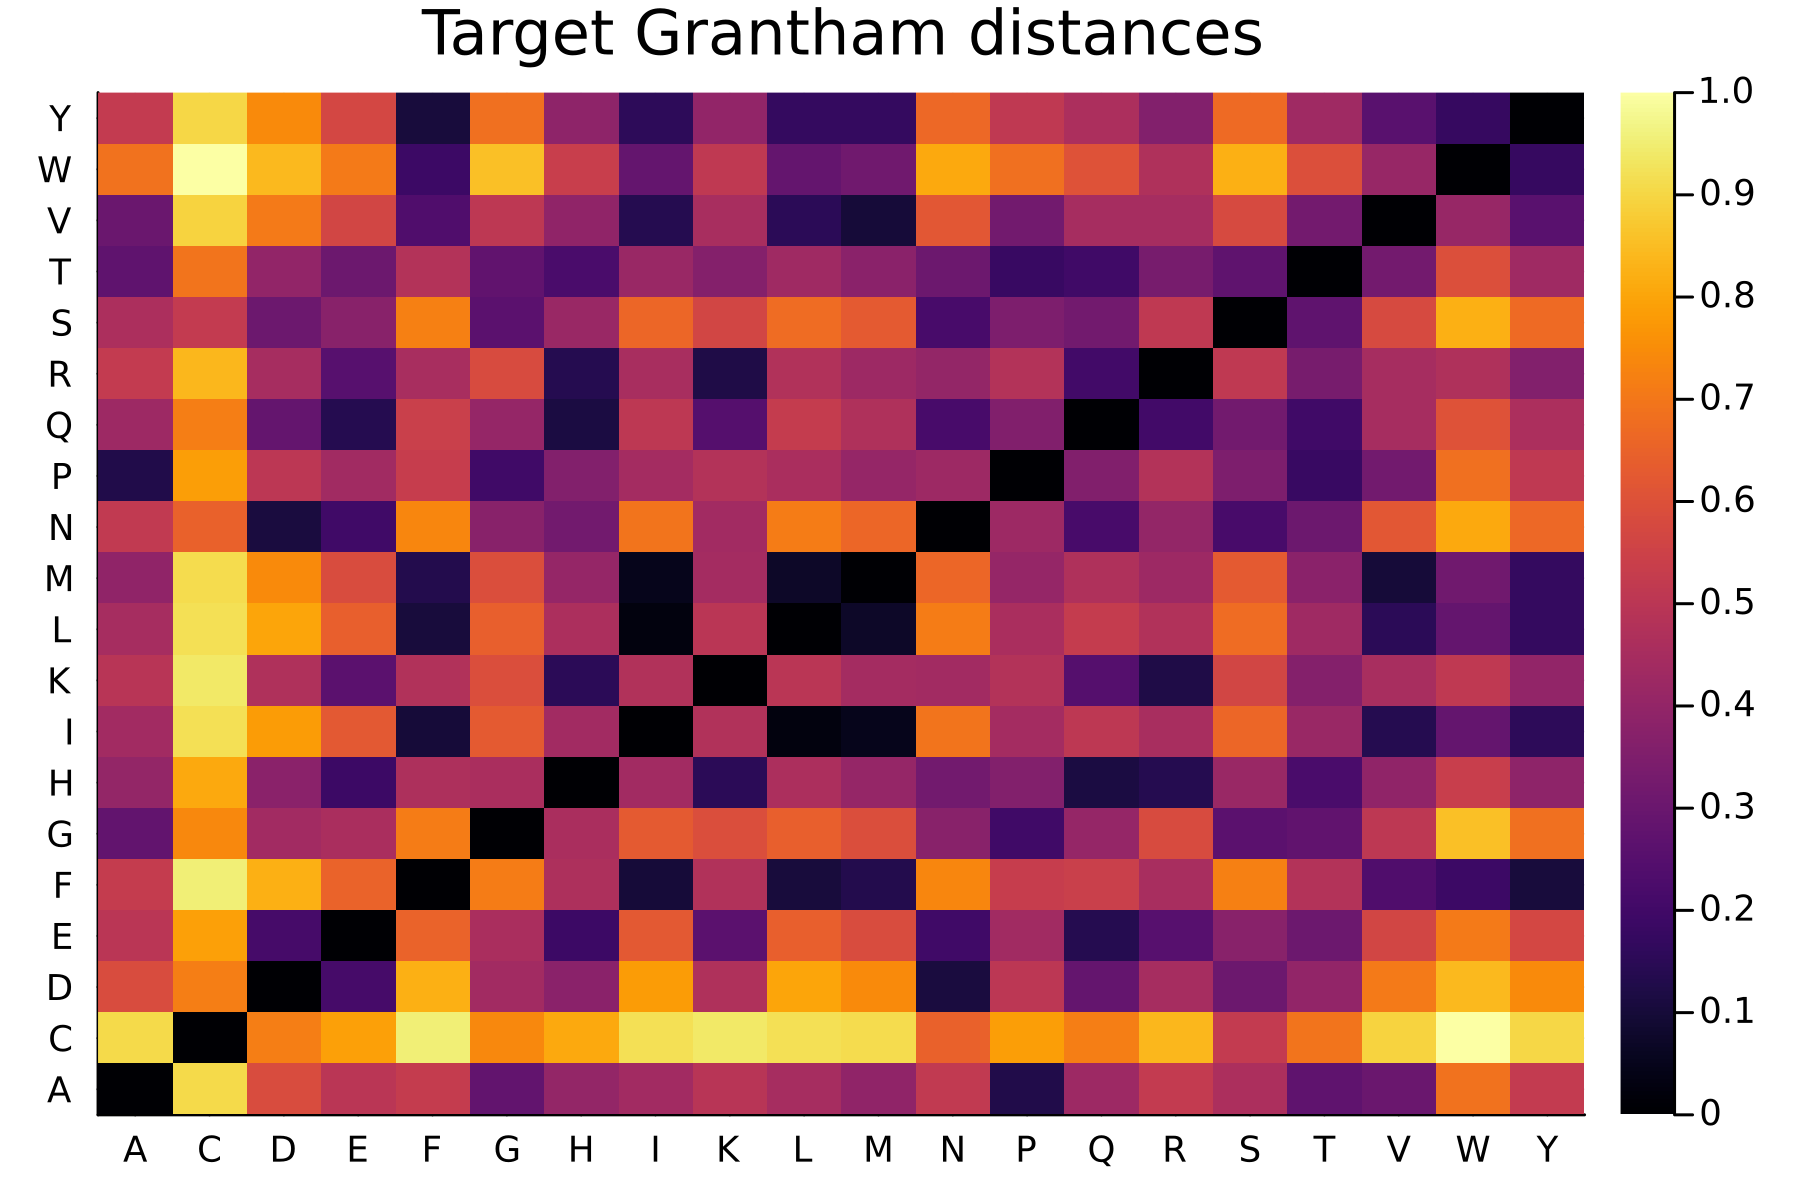
\includegraphics[width=\textwidth]{granttarget.png}
        \caption{Normalized Grantham's distance matrix.}
        \label{fig:grant}
    \end{subfigure}
\end{minipage}
\\
\centering
    \begin{minipage}[b]{.5\textwidth}
    \begin{subfigure}[b]{\textwidth}
        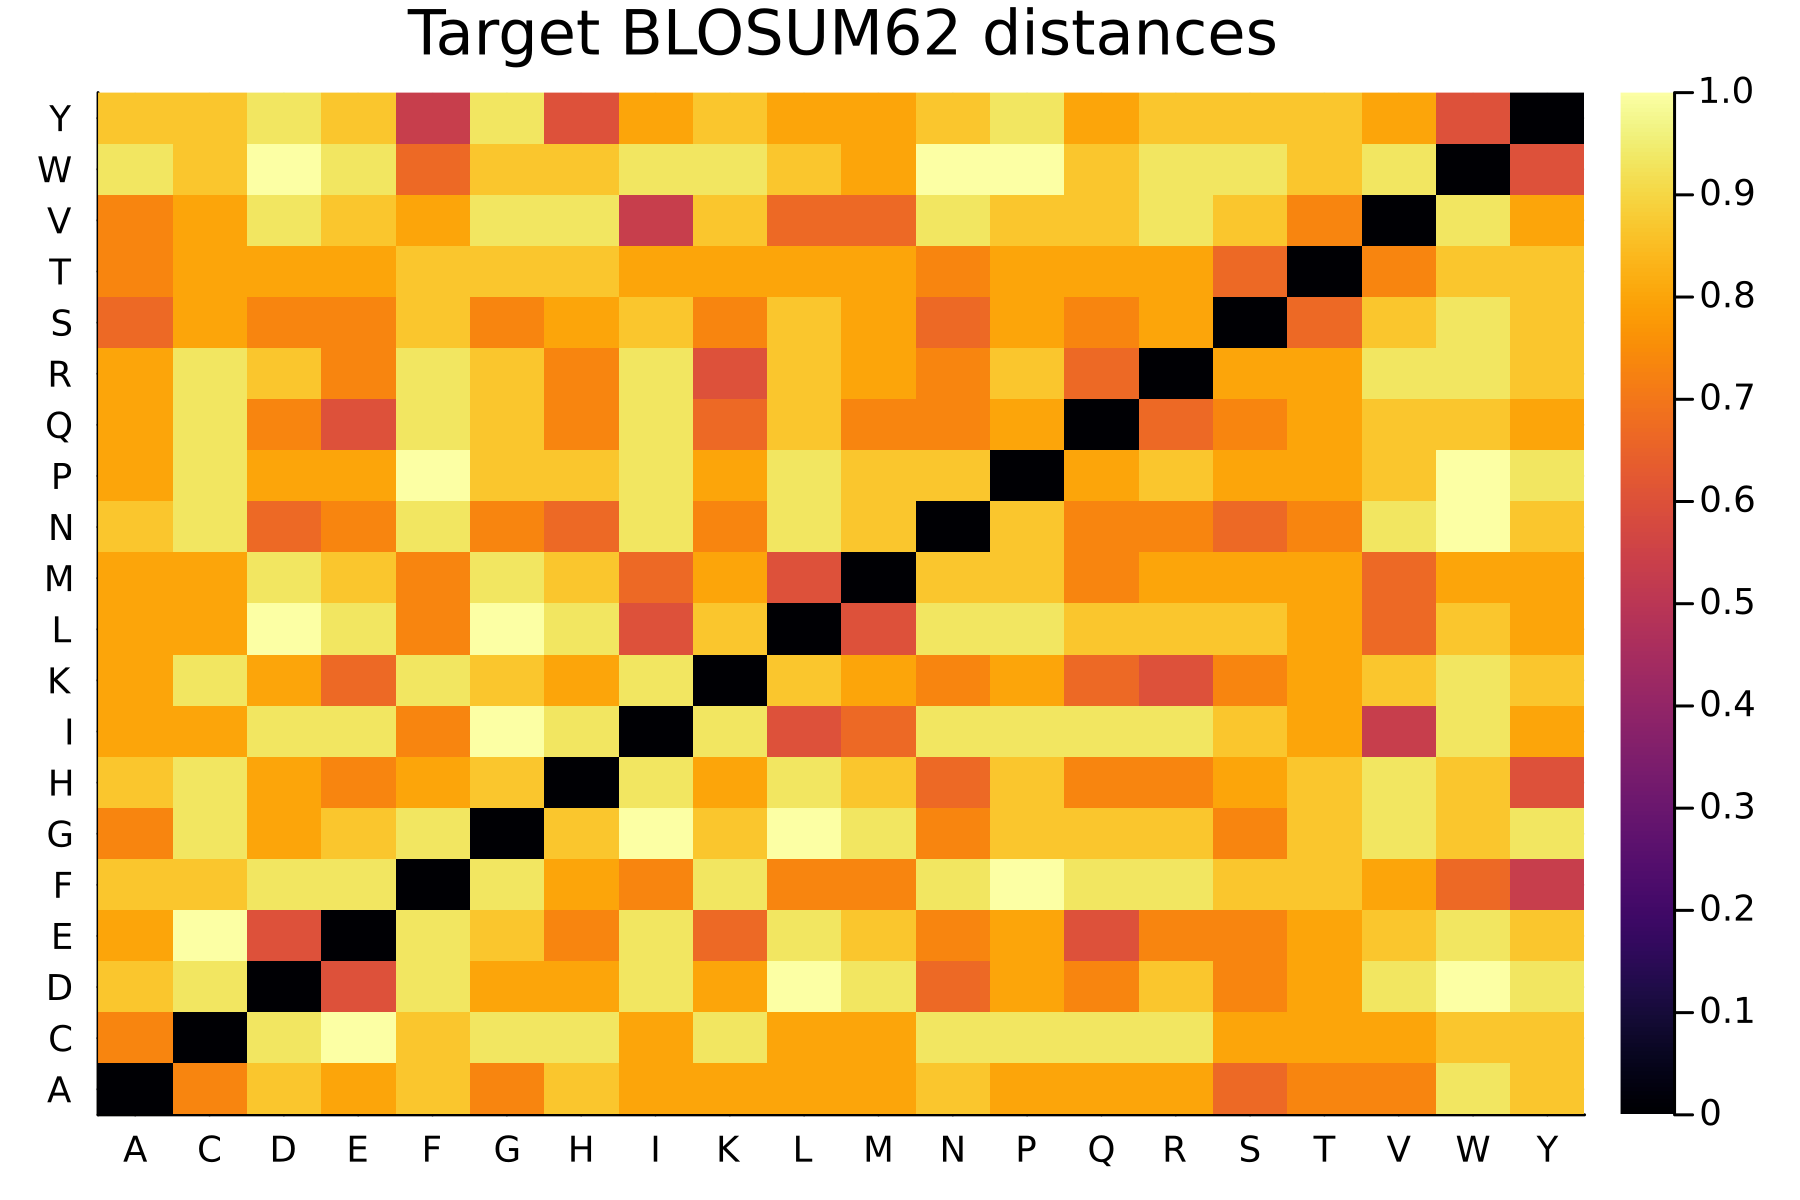
\includegraphics[width=\textwidth]{blosumtarget}
        \caption{Normalized amino acid distance matrix based on BLOSUM62.}
        \label{fig:blosum}
    \end{subfigure}
    \end{minipage}
\\
\centering
    \begin{minipage}[b]{.5\textwidth}
    \begin{subfigure}[b]{\textwidth}
        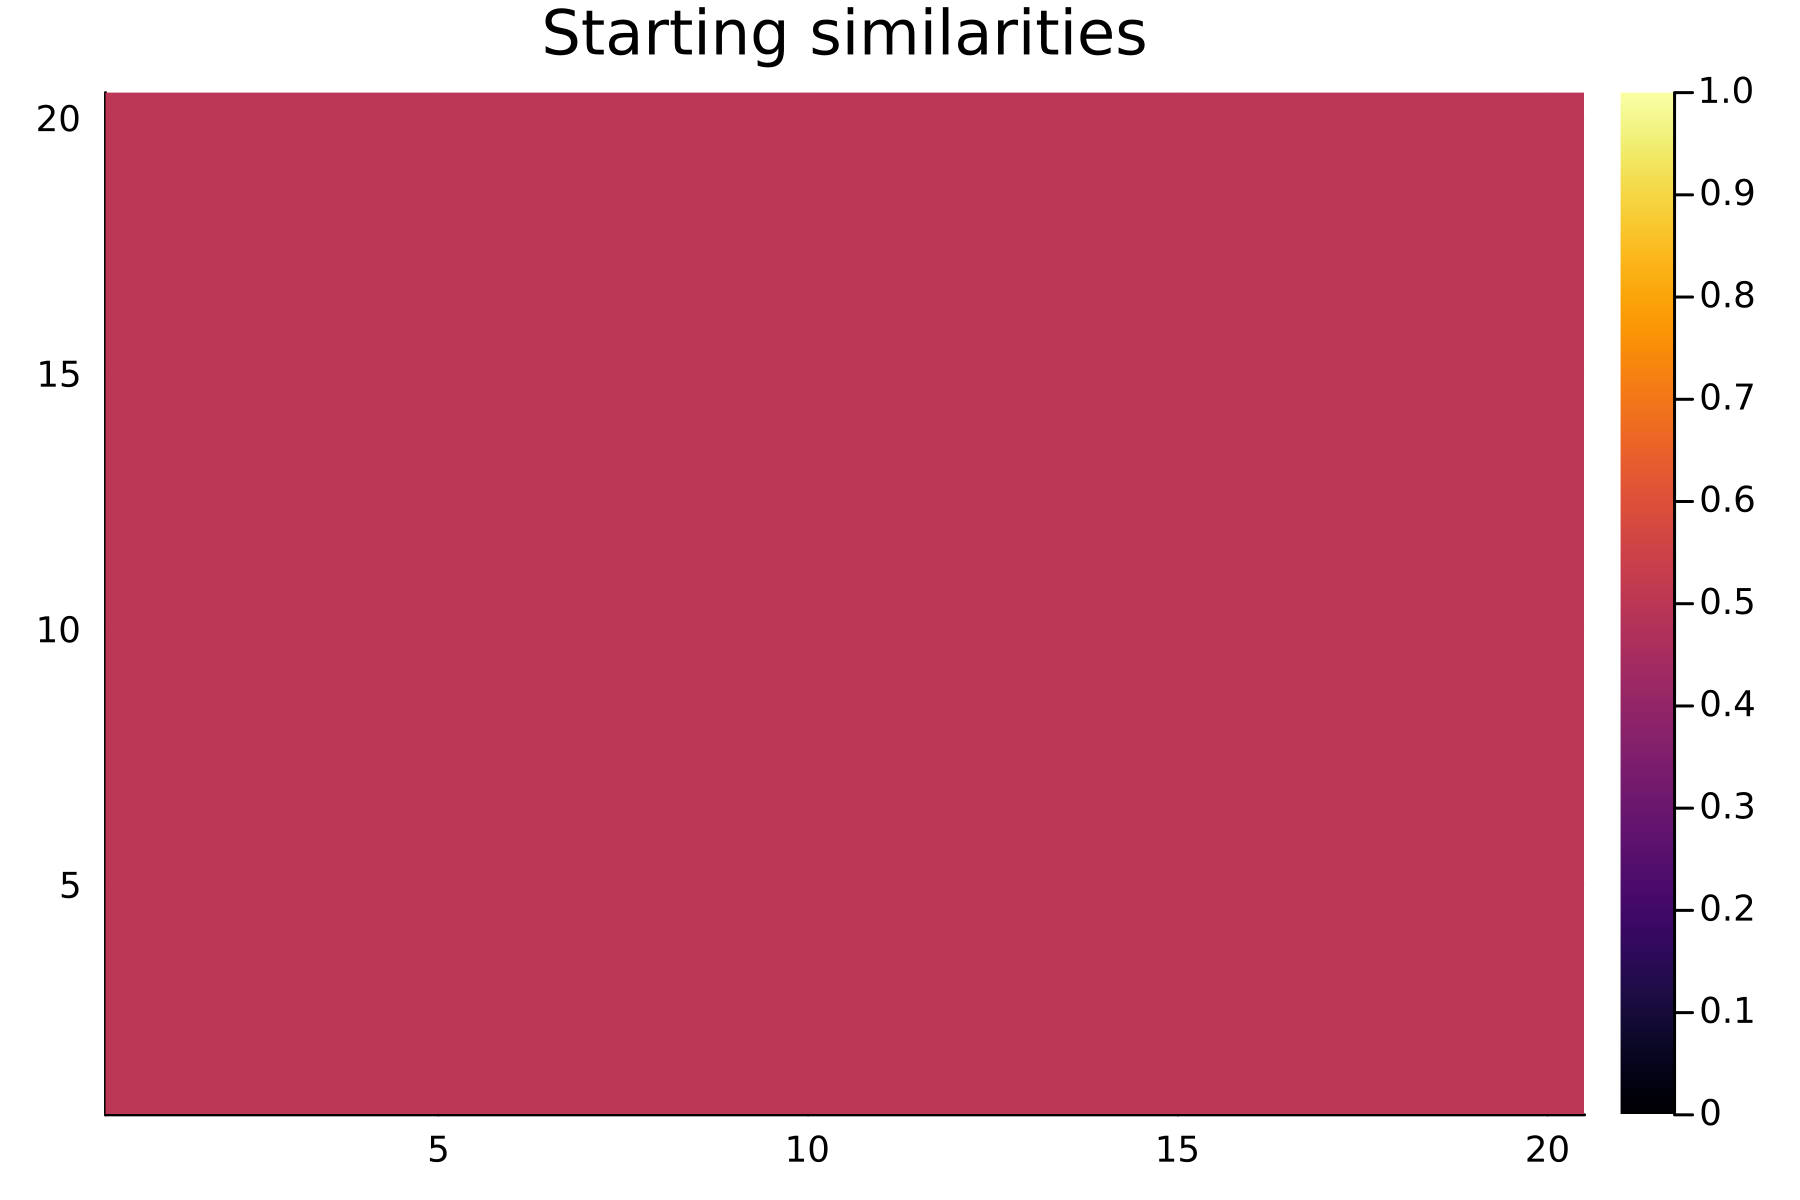
\includegraphics[width=\textwidth]{random}
        \caption{Achieved similarity matrix.}
        \label{fig:random}
    \end{subfigure}
    \end{minipage}
    \caption{Heatmap of the target pairwise amino acid distances, based on (a) Grantham's distance matrix (b) BLOSUM62 matrix and heatmap of (c) the achieved distances.}
    \label{fig:ga}
\end{figure}
\subsection*{Contextualized neighborhood-encoding of amino acids}
Looking at the average neighborhood-encoded amino acids starting from ESM-2 embeddings and the human proteome (figures \ref{fig:AAtr4} and \ref{fig:AAtr50}), the charged amino acids seem to be grouped vertically by PC 2, roughly dividing the polar and non-polar amino acids, albeit slightly more pronounced for $n = 50$. Also interesting, to see very similar groupings in the PCA plots might indicate that the first four amino acids before and after a residue are the most crucial.

The PCA scatter plots generated from random vectors (figures \ref{fig:AArtr4} and \ref{fig:AArtr50}) show slightly different results as compared to the ones starting from ESM embeddings. These PCAs also capture less variance, which may indicate that encoding biological information/similarities into the vectors beforehand might be useful. For $k = 4$, some typicalities are noticed such as the close grouping of the negatively charged amino acids (D and E) and the consistent triangular grouping of H, L and R. Nonetheless, for $k = 50$ with random vectors, we see results deviating from all the PCA scatter plots of other neighborhood-encoded amino acids, which could mean that a PCA is not able to capture the sparse information for this case or that these vectors might be oversaturated.

\begin{figure}[H]
    \centering
    \begin{subfigure}[b]{0.45\textwidth}
        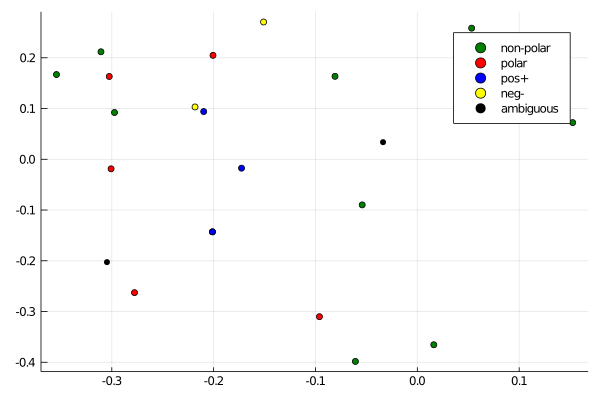
\includegraphics[width=\linewidth]{4tr_emb}
        \caption{$n = 4$ from projected ESM-2 embeddings, accounting for 21 \% of the total variance.}
        \label{fig:AAtr4}
    \end{subfigure}
    \hfill
    \begin{subfigure}[b]{0.45\textwidth}
        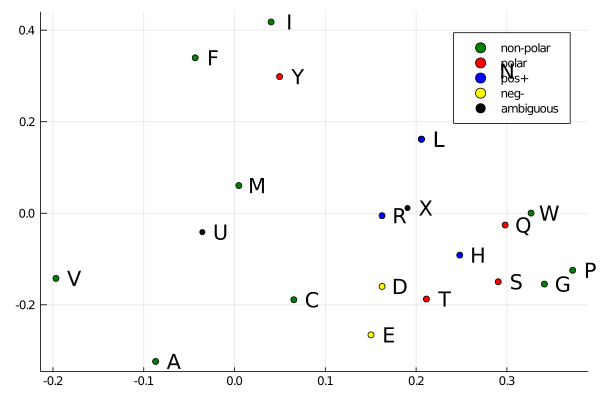
\includegraphics[width=\linewidth]{50tr_emb}
        \caption{$n = 50$ from projected ESM-2 embeddings, accounting for 21 \% of the total variance.}
        \label{fig:AAtr50}
    \end{subfigure}
    \vspace{10pt} % Add vertical space between rows
    \begin{subfigure}[b]{0.45\textwidth}
        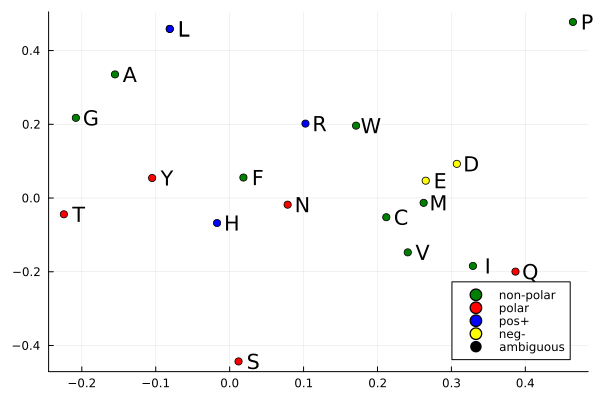
\includegraphics[width=\linewidth]{r4tr_emb}
        \caption{$n = 4$ from random vectors, accounting for 11 \% of the total variance.}
        \label{fig:AArtr4}
    \end{subfigure}
    \hfill
    \begin{subfigure}[b]{0.45\textwidth}
        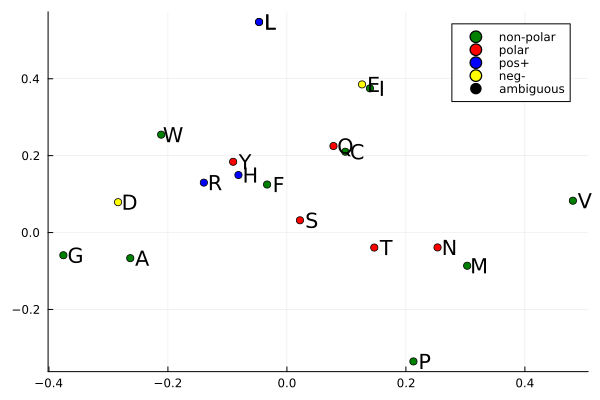
\includegraphics[width=\linewidth]{r50tr_emb}
        \caption{$n = 50$ from random vectors, accounting for 11 \% of the total variance.}
        \label{fig:AArtr50}
    \end{subfigure}
    \caption{Scatter-plots of the first two principal components of the average amino acid HDVs with neighborhood-information of $n = 4$ and $n = 50$ encoded, learned from the human reference proteome. The top row represents encoded amino acids starting from projected ESM-2 embeddings, and the bottom row represents encoded amino acids starting from random hyperdimensional vectors. The amino acids are annotated and colored based on their chemical property of polarity.}\label{fig:bigfig}
\end{figure}

\section{Discussion}\label{sec:dis3}
In Rives \textit{et al.} (2011), they conducted a similar experiment with their transformer model~\cite{esm1}. Our results are comparable to theirs, but not as cleanly grouped which is likely due to several factors. For instance, due to the intrinsic stochastic nature of hyperdimensional computing, it is prone to capture some amount of noise. On top of this, it is difficult for dimensionality-reduction methods such as PCA to accurately capture the intricacies of 10,000-dimensional vectors into 2 dimensions. UMAP projections were also made for the resulting vectors of the neighborhood-encoder method, shown in appendix A, but these did not reveal any new information. For specifically the neighborhood-encoder method, the amount of data we used is not comparable to theirs: our method learned from less than 21000 sequences whilst their model was trained on 250 million sequences. They also included sequences originating from all recorded organisms in the UniProt database at that time whilst we confined ourselves to human sequences. Secondly, hyperdimensional vectors have a limited capacity, meaning long-range dependencies of a residue will saturate the hyperdimensional vector depending on the range.

We can predict the angle between a bundled vector and a randomly selected vector from said bundle vector by $\Theta = \arccos({2k \choose k}/2^{2k})$ with $2k+1$ equal to the number of sequences in the class~\cite{sathdv}. This approximation is valid for bipolar/binary vectors in hyperdimensions $(\ge 10000)$. This equation also suggests that an increase in dimensions will not influence the angle. Evaluating this equation by considering random 1001 vectors in a bundled vector, so $k = 500$, results in an angle of $88.6^{\circ}$. This indicates that a vector has a limited capacity: the more vectors we bundle together, the closer the angle will be to $90^{\circ}$ and thus the more dissimilar the bundled vector becomes to its components. This results in the bundled vectors not being representative anymore of a given dataset. This equation assumes that the bundled vector is a bundle of purely random vectors which is not the case for most of our embeddings; however, it provides us a rough idea about the bundling capacity of a hyperdimensional vector warranting further research in this domain.

In the forthcoming two chapters, we will delve into practical case studies that draw upon the methodologies expounded in this chapter, engaging with protein sequence datasets and executing predictive tasks therein. Chapter 4 is focussed on exploring classification tasks employing protein sequence embeddings, wherein we will research the power of hyperdimensional computing, whether or not together with established machine learning methods. In chapter 5, we shift our focus toward the classification tasks on amino acid vectors by using our neighborhood-encoder method to create contextualized embeddings of amino acids and neural networks to classify these.
\chapter[PhaLP case study: Hyperdimensional protein sequence embedding and binary protein-level classification]{PhaLP case study:\\Hyperdimensional protein sequence embedding\\and binary protein-level classification}
\section{PhaLP database}
To implement and evaluate hyperdimensional computing in typical problem settings in computational biology, the potential of hyperdimensional computing will be evaluated on the PhaLP dataset~\cite{phalp} in this chapter. PhaLP is a comprehensive database currently comprising more than 17,000 entries of phage lytic proteins, including much of their information such as their type, domains and tertiary structures. Phage lytic proteins are used by bacteriophages to infect bacterial cells. To cross the bacterial cell walls, phages use two different types of phage lytic proteins: virion-associated lysins (VALs) and endolysins. Phage lytic proteins also comprise one or more functional domains categorized into two classes: enzymatically active domains (EADs) and cell wall binding domains (CBDs)~\cite{phage}.

The escalating global antibiotic resistance crisis has necessitated the development of alternative strategies to combat bacterial infections~\cite{antibiotic}. One such promising alternative is enzybiotics, a class of enzyme-based antibiotics derived from phage lytic proteins. Phage lytic proteins are produced by bacteriophages during their lytic replication cycle and are responsible for breaking down the bacterial cell wall. As these proteins exhibit a high level of diversity, it is critical to make well-informed selections during the early stages of research and development. In response to this need, Criel \textit{ et al.} introduced PhaLP~\cite{phalp}, a comprehensive, automatically updated, and easily accessible database containing more than 17,000 phage lytic proteins. PhaLP aims to serve as a portal for researchers, allowing them to access all relevant information about the current diversity of phage lytic proteins through user-friendly search engines. This database is specifically designed to facilitate the development and application of enzybiotics by providing a wealth of data on protein architecture, evolution, and bacterial hosts corresponding to the phages. PhaLP not only serves as a valuable starting point for the broad community of enzybiotic researchers but also offers continually improving evolutionary insights that can act as a natural inspiration for protein engineers. By enabling researchers to make well-considered selections of phage lytic proteins during the early stages of their projects, PhaLP plays a significant role in the development of highly effective, narrow-spectrum antibiotics. These enzybiotics have the potential to revolutionize the field of antibacterial agents, offering a much-needed response to the alarming threat of antibiotic resistance that plagues healthcare systems worldwide.

To fully utilize the rich content of PhaLP, the researchers conducted a series of analyses at three levels to gain insights into the host-specific evolution of phage lytic proteins. First, they provided an overview of the modular diversity of these proteins. This was followed by the adoption of data mining and interpretable machine learning approaches to reveal host-specific design rules for domain architectures in endolysins. Lastly, the evolution of phage lytic proteins at the protein sequence level was explored, uncovering host-specific clusters.

In this chapter, we will explore the authors' experiment on protein classification based on sequence data and evaluate the potential of hyperdimensional computing in the context of protein functional annotation. The primary objective is to better understand the role of hyperdimensional computing in protein classification and to elucidate its potential advantages over conventional machine learning techniques.

\section{Type classifcation}
The developers of PhaLP aimed to classify protein sequences based on their type, with a focus on two types of phage lytic proteins: virion-associated lysins (VALs) and endolysins. Both of these proteins play crucial roles in the lytic replication cycle of bacteriophages, as they help the viruses breach the bacterial cell wall. VALs are an integral component of the viral particle, and their primary function is to create a small pore in the peptidoglycan layers of the bacterial cell wall at the infection site. This process allows the bacteriophage to gain access to the interior of the bacterial cell, initiating the lytic replication cycle. On the other hand, endolysins are produced within the infected bacterial cell and act toward the end of the replication cycle. These enzymes degrade the peptidoglycan layer of the bacterial cell wall, leading to cell lysis and the release of new viral particles~\cite{phalp}.

Only a fraction of the database is manually annotated to include the protein's type because the amount of phage lytic proteins whose type is described in the literature is relatively small. The developers of PhaLP resorted to a machine learning approach for the classification of unannotated sequences. The authors embedded each protein sequence \textit{via} SeqVec~\cite{seqvec} and trained a random forest classifier~\cite{randomforest} with 100 estimators and balanced weights to classify the proteins whose types were unknown. For this case study, we attempted to simulate their experiments of classifying the proteins into the two types based on their sequence using several techniques based on hyperdimensional computing.

\section{Methods}
As of March 2023, the latest version of the PhaLP database,~\textit{v2021\_04}, has been used to test our models. This dataset consists of 17,356 unique amino acid sequences of phage-lytic proteins.
\subsection*{Embedding of sequences into hyperdimensional vectors}
First, we used the two sequence encoding techniques as discussed in Section~\ref{ssec:protseq} to embed the protein sequences in hyperdimensional space. These methods have been applied to all sequences in the dataset that were manually annotated on their type using both random hyperdimensional vectors and projected ESM-2 embeddings. These were then visually assessed \textit{via} PCA. To confirm the diversity of sequences within the types, pairwise global alignments of every possible non-ambiguous combination of sequences within the two types were performed using the BioAlignments.jl package with a BLOSUM62 scoring matrix and -5 penalty for gaps. All scores within a type are then averaged out.

\subsection*{Classification of hyperdimensional protein sequence embeddings}
To discriminate, we experimented with 3 different methods: the rudimentary hyperdimensional computing classification as seen in section~\ref{sec:example}, an XGBoost classifier and  by A. Hernandez-Cano~\textit{et al.}~\cite{onlinehd}. As in the PhaLP study, we use all non-ML annotated proteins in the dataset. Out of the 11549 unambiguous UniParc accessions in the newest version of the database, 4829 are manually annotated on their type. Out of these manually annotated proteins, 2803 are endolysins and 2026 are VALs. For all classification tests, the F1-score is used as a performance metric as we want to measure the overall performance of the methods. The F1-score is the harmonic mean of the precision and recall and could be interpreted as a weighted accuracy. This accounts for the slight unbalance in the dataset. All methods were evaluated \textit{via} a stratified 10-fold cross validation.
\subsubsection*{Naive additive method}
As a baseline level, we use the rudimentary HDC classification technique as seen in Section~\ref{sec:example}: the binary HDVs of sequences of the same class are bundled to construct single HDVs representative of every class. Then, a sequence's class is inferred by comparing the sequence's HDV to both class HDV \textit{via} a similarity measure based on the assumption that the class vector is maximally similar to its components.
\subsubsection*{XGBoost classifier}
The baseline hyperdimensional classification method has been compared to a more established method, the XGBoost classifier~\cite{xgboost}. The classification with an XGBoost classifier is done via the default XGBoost classifier from \textit{XGBoost.jl v2.2.5} using the binary hyperdimensional embeddings as an input.
\subsubsection*{OnlineHD methods}
Another method we experimented with, is OnlineHD by A. Hernandez-Cano~\textit{et al.}~\cite{onlinehd}. It is an algorithm that expands on the classical hyperdimensional training methods by trying to eliminate model saturation. Instead of naively bundling vectors on top of each other, this algorithm assigns weights to every addition depending on how much new information it adds to the model to prevent class vector saturation. To train the model, assume a new data point $V$ with label $l$ and class vectors $C_{i}$ with each having a label $i$. The cosine similarity of $V$ with every class vector is then calculated (denoted as $cos(V, C_{i})$ with $i$ being a label). If $V$ with an actual label $l$ would have been predicted as $l'$, the class vectors will be updated as followed (with learning rate $\eta$ as a tunable hyperparameter):

\begin{alignat}{1}
    \label{eqn:onlinehd}
    C_{l} &\leftarrow C_{l} + \eta (1 - cos(V , C_{l})) * V \\
    C_{l'} &\leftarrow C_{l'} - \eta (1 - cos(V, C_{l'})) * V
\end{alignat}

This means that if a new data point is highly dissimilar to its class vector and thus contains a high amount of new information, the weight of the update ($\eta (1 - cos(V, C_{i}))$) will be high. The information is then also subtracted from the incorrectly predicted class vector. If a label would be correctly predicted for a new data point, the model will not be updated to avoid saturation. To initialize the model, the first vector of a class to be assessed is assumed to be the class vector. For example, if a query vector in our dataset is predicted to be a VAL, but its actual label is endolysin, the class vectors are then updated as followed:

\begin{alignat}{1}
    \label{eqn:onlinehd2}
    C_{VAL} &\leftarrow C_{VAL} + \eta (1 - cos(V, C_{VAL})) * V \\
    C_{endo} &\leftarrow C_{endo} - \eta (1 - cos(V, C_{endo})) * V
\end{alignat}

Due to the nature of this model, we cannot constrict our hyperdimensional embeddings to a bipolar or binary nature anymore and the embeddings are thus allowed to be real-numbered. Mathematical operations such as multiplications and additions are then assumed to be element-wise. On top of the single-pass method as discussed above, A. Hernandez-Cano~\textit{et al.} also implemented an iterative retraining algorithm to increase the accuracy of OnlineHD. This starts from the class vectors made \textit{via} the single-pass OnlineHD model, but assesses the class vectors by performing inference with every training vector. If a training vector's label is wrongly predicted, equations 4.1 and 4.2 are then used to update the model. This entire sequence is iterated over a given amount of cycles.

Since these algorithms are only available as PyTorch implementations, implementations in Julia have been made here. A stratified 10-fold cross validation of these models with our subject sequences has been performed. The learning rate is set at 0.035 for both the single-pass and the iterative method and the amount of retraining iterations for the iterative method is set to 120 as these are the values set by default in their PyTorch package. To test these algorithms, real-numbered embeddings had to be made from our subject sequences. So instead of embedding the sequences starting with random bitvectors, random vectors with values in interval $[-1, 1]$ for both the random amino acid vectors and projected ESM-2 embeddings were made to obtain real-valued hyperdimensional vectors for every amino acid. The same bag-of-words and convolutional approaches as discussed in Section~\ref{ssec:protseq} have been applied here to obtain real-valued sequence embeddings. These were assessed \textit{via} a scatter-plot of the two first principal components of their PCA projection.

To monitor the training procedure of an OnlineHD single-pass model, the same procedures as above are followed, but without the cross validation. The absolute difference between the cosine similarities, $cos(V, C_{VAL})$ and $cos(V, C_{VAL})$ as described in equations 4.3 and 4.4, has then been calculated for each query vector before the update. The results are shown in Figure~\ref{fig:main2} for every combination of amino acid- and sequence embedding methods. Another approach to monitor the training procedure is to track the two class vectors $C_{VAL}$ and $C_{endo}$ individually. For each query vector $V_{l}$ with a known label $l$, we calculate the cosine similarity $cos(V_{l}, C_{l})$. The results are shown in Figure~\ref{fig:main} for every combination of amino acid- and sequence embedding methods. 

To follow the training procedure in terms of performance, the dataset is divided into training and testing sets, while ensuring stratification is preserved, with the test set comprising 10 \% of the data. The training data is further partitioned into 500 batches, and the model is trained incrementally using these batches. After each batch has been processed, the model's performance on the test data is assessed to provide insights into its learning trajectory with the results shown in Figure~\ref{fig:main39} for every combination of amino acid- and sequence embedding methods.

\section{Results}
\subsection*{Embedding of sequences into hyperdimensional vectors}
There is no visual difference between the PCA plots for the sequences embedded \textit{via} the bag-of-words method and the convolutional method, but there is a clear difference between the different starting embeddings as seen in Figure~\ref{fig:phalp_emb}. The binary sequence embeddings from both the bag-of-words method and the convolutional method made with ESM-2 AA embeddings seem to capture more of the variance between the sequences.

\begin{figure}[ht!]
    \centering
    \begin{subfigure}{0.48\textwidth}
        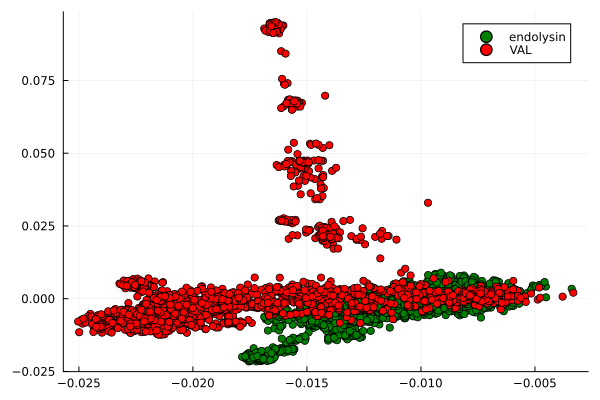
\includegraphics[width=\textwidth]{phalp_bow_rand}
        \caption{BoW-encoded protein sequences, starting from random vectors. These PCs account for roughly 7 \% of the total variance in the system.}
    \label{fig:phalpbowrand}
    \end{subfigure}
    \hfill
    \begin{subfigure}{0.48\textwidth}
        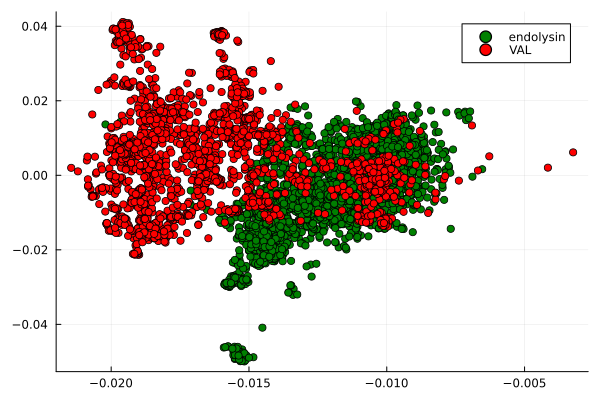
\includegraphics[width=\textwidth]{phalp_bow_esm}
        \caption{BoW-encoded protein sequences, starting from projected ESM-2 embeddings. These PCs account for roughly 15.5 \% of the total variance in the system.}
    \label{fig:phalpbowesm}
    \end{subfigure}
    
    \begin{subfigure}{0.48\textwidth}
        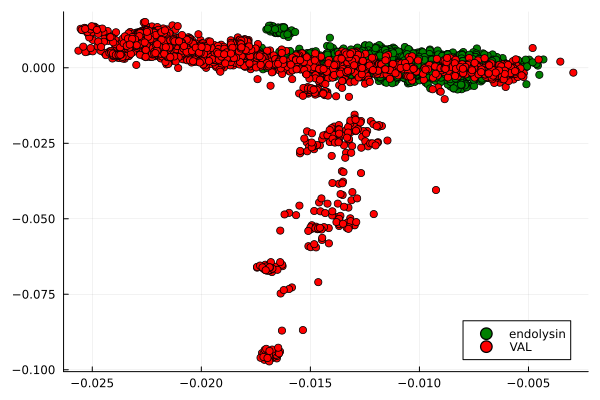
\includegraphics[width=\textwidth]{phalp_cnn_rand}
        \caption{Convolutionally encoded protein sequences, starting from random vectors. These PCs account for roughly 7 \% of the total variance in the system.}
    \label{fig:phalpcnnrand}
    \end{subfigure}
    \hfill
    \begin{subfigure}{0.48\textwidth}
        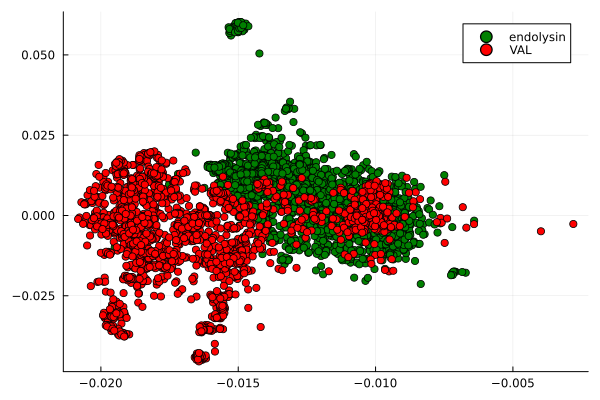
\includegraphics[width=\textwidth]{phalp_cnn_esm}
        \caption{Convolutionally encoded protein sequences, starting from random vectors. These PCs account for roughly 15.5 \% of the total variance in the system.}
    \label{fig:phalpcnnesm}
    \end{subfigure}
    \caption{Scatter-plot of the first two principal components of the binary encoded phage lytic proteins \textit{via} the BoW-method starting from (a) random HDVs per amino acid (b) projected ESM-2 amino acid embeddings and \textit{via} the convolutional method from (c) random HDVs per amino acid (d) projected ESM-2 amino acid embeddings. Only manually annotated phage lytic proteins were considered and are color-coded based on their type.}
    \label{fig:phalp_emb}
\end{figure}

As with the binary embeddings, PCA of the real-valued sequence embeddings shows no distinction between those made \textit{via} the bag-of-words method and the convolutional method whilst showing a clear difference between the different starting embeddings as seen in Figure 4.3. Similarly, the explained variance is much higher for embeddings made with projected ESM-2 embeddings. However, the PCA method retrieves much more information from real-valued embeddings. From all the PCA scatter plots mentioned, we can estimate by the sparser distribution of the VAL proteins that these would be slightly more diverse in sequence than endolysins.

\begin{figure}[ht!]
    \centering
    \begin{subfigure}[b]{0.48\textwidth}
        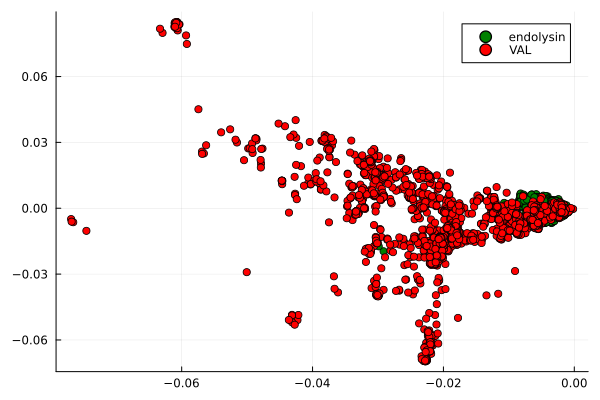
\includegraphics[width=\textwidth]{phalp_bow_rand_real}
        \caption{BoW-encoded protein sequences, starting from random vectors. These PCs account for roughly 30.4 \% of the total variance in the system.}
    \label{fig:phalpbowrandr}
    \end{subfigure}
        \hfill
    \begin{subfigure}[b]{0.48\textwidth}
        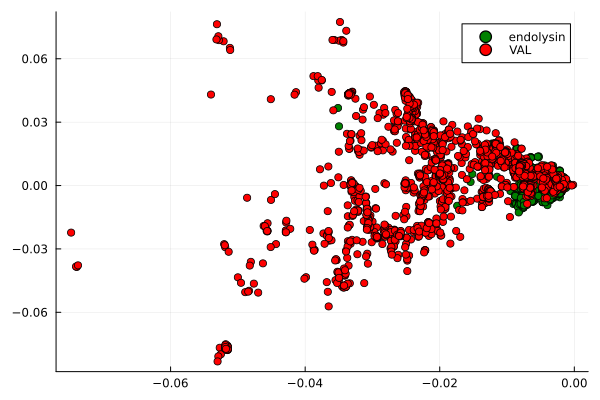
\includegraphics[width=\textwidth]{phalp_bow_esm_real}
        \caption{BoW-encoded protein sequences, starting from projected ESM-2 embeddings. These PCs account for roughly 57.3 \% of the total variance in the system.}
    \label{fig:phalpbowesmr}
    \end{subfigure}
    \begin{subfigure}[b]{0.48\textwidth}
        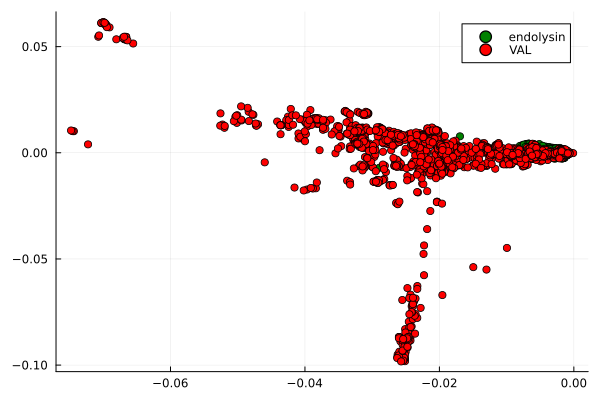
\includegraphics[width=\textwidth]{phalp_rand_esm_real}
        \caption{Convolutionally encoded protein sequences, starting from random vectors. These PCs account for roughly 30.4 \% of the total variance in the system.}
    \label{fig:phalpcnnrandr}
    \end{subfigure}
    \hfill
    \begin{subfigure}[b]{0.48\textwidth}
        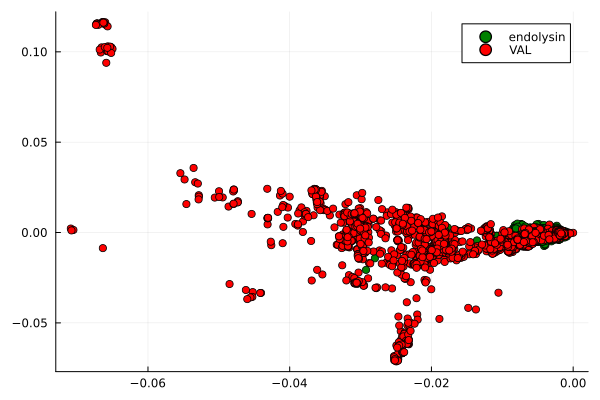
\includegraphics[width=\textwidth]{phalp_cnn_esm_real}
        \caption{Convolutionally encoded protein sequences, starting from projected ESM-2 embeddings. These PCs account for roughly 57.3 \% of the total variance in the system.}
    \label{fig:phalpcnnesmr}
    \end{subfigure}
    \caption{Scatter-plot of the first two principal components of the real-valued encoded phage lytic proteins \textit{via} the BoW-method starting from (a) random HDVs per amino acid (b) projected ESM-2 amino embeddings and \textit{via} the convolutional method from (c) random HDVs per amino acid (d) projected ESM-2 amino embeddings. Only manually annotated phage lytic proteins were considered and are color-coded based on their type.}\label{fig:phalp_embr}
\end{figure}

In each of the PCA projections previously discussed, VALs consistently exhibited a higher degree of diversity in comparison to endolysins. To validate this observation, pairwise alignments were conducted across all sequences within their respective groups. VAL proteins yielded an average score of -209, while the endolysins scored -7. This pronounced disparity in scores shows greater intra-group dissimilarity among the VAL sequences as opposed to those of the endolysins, confirming our findings in the PCA projections.

\subsection*{Classification of hyperdimensional protein sequence embeddings}
The resulting F1-scores from our 4 classification methods are listed in Table~\ref{tab:phalpclass}. Evaluating our naive additive model using stratified 10-fold cross-validation results in F1-scores of around 0.14 for every kind of amino acid embedding.

\begin{table}[h]
    \caption{\label{tab:phalpclass}Results of type classifications using the principal classification technique of hyperdimensional computing, an XGBoost classifier and OnlineHD implementations with several kinds of embeddings. Note that the OnlineHD-based models were developed using real-valued embeddings.}
    \resizebox{\textwidth}{!}{\begin{tabular}{ccccc}
        \hline
        \underline{F1-scores} & \textbf{BoW/random} & \textbf{BoW/ESM} & \textbf{Convolutional/random} & \textbf{Convolutional/ESM} \\
        \hline
        \textbf{Naive addition} & 0.1458 & 0.1468 & 0.1461 & 0.1461 \\
        \hline
        \textbf{XGBoost classifier} & 0.9667 & 0.9754 & 0.9661 & 0.986 \\
        \hline
        \textbf{Single-pass OnlineHD} & 0.8901 & 0.9214 & 0.7793 & 0.8400 \\
        \hline
        \textbf{Iterative OnlineHD} & 0.9487 & 0.9757 & 0.9486 & 0.9670 \\
        \hline
    \end{tabular}}
\end{table}

The scores of the XGBoost classifier with our sequence embeddings are much more comparable to the results of the experiment in the PhaLP paper, with the convolutional embeddings generally performing better than the bag-of-words embeddings and also the ESM 2-based performing better than random base vectors when considering the type of amino acid vectors used. This is an indication that hyperdimensional computing can provide a very fast and reliable method of embedding protein sequences, even without prior biological information. The drawback of this machine learning model, which is to be expected from every gradient-based model, is that training and predictions take much longer to compute compared to hyperdimensional training models. The cross validation procedure took up to 5 minutes on a consumer-grade laptop, whilst with the naive additive approach, the procedure took less than 10 seconds to finish.

Comparing the results of the OnlineHD models to the naive additive HDC model, we can see a substantial increase in the performance of this model. The single-pass model seems to have more widely varying results depending on the type of embeddings used. As opposed to the XGBoost classifier, it performs better using bag-of-words embeddings. The model also performs better when trained with embeddings based on projected ESM-2 vectors. Iterative retraining of the model seems to increase its performance significantly, even coming close to the performance of an XGBoost classifier in this case. Further improvement might be found when optimizing the models' parameters. The cross validation procedure takes less than 10 seconds to run for the single-pass model, whilst doing an iterative retraining of the model adds 2 to 3 minutes. This model appears to be a decently performing extension of the rudimentary hyperdimensional classification model for protein classification, whilst still being much more efficient than the commonly used machine learning models. The drawback of the model is that we cannot use hyperefficient bit-operations anymore, which limits its efficiency compared to the binary nature of the additive model.

\begin{figure}[ht!]
    \centering
    \begin{subfigure}{0.48\textwidth}
        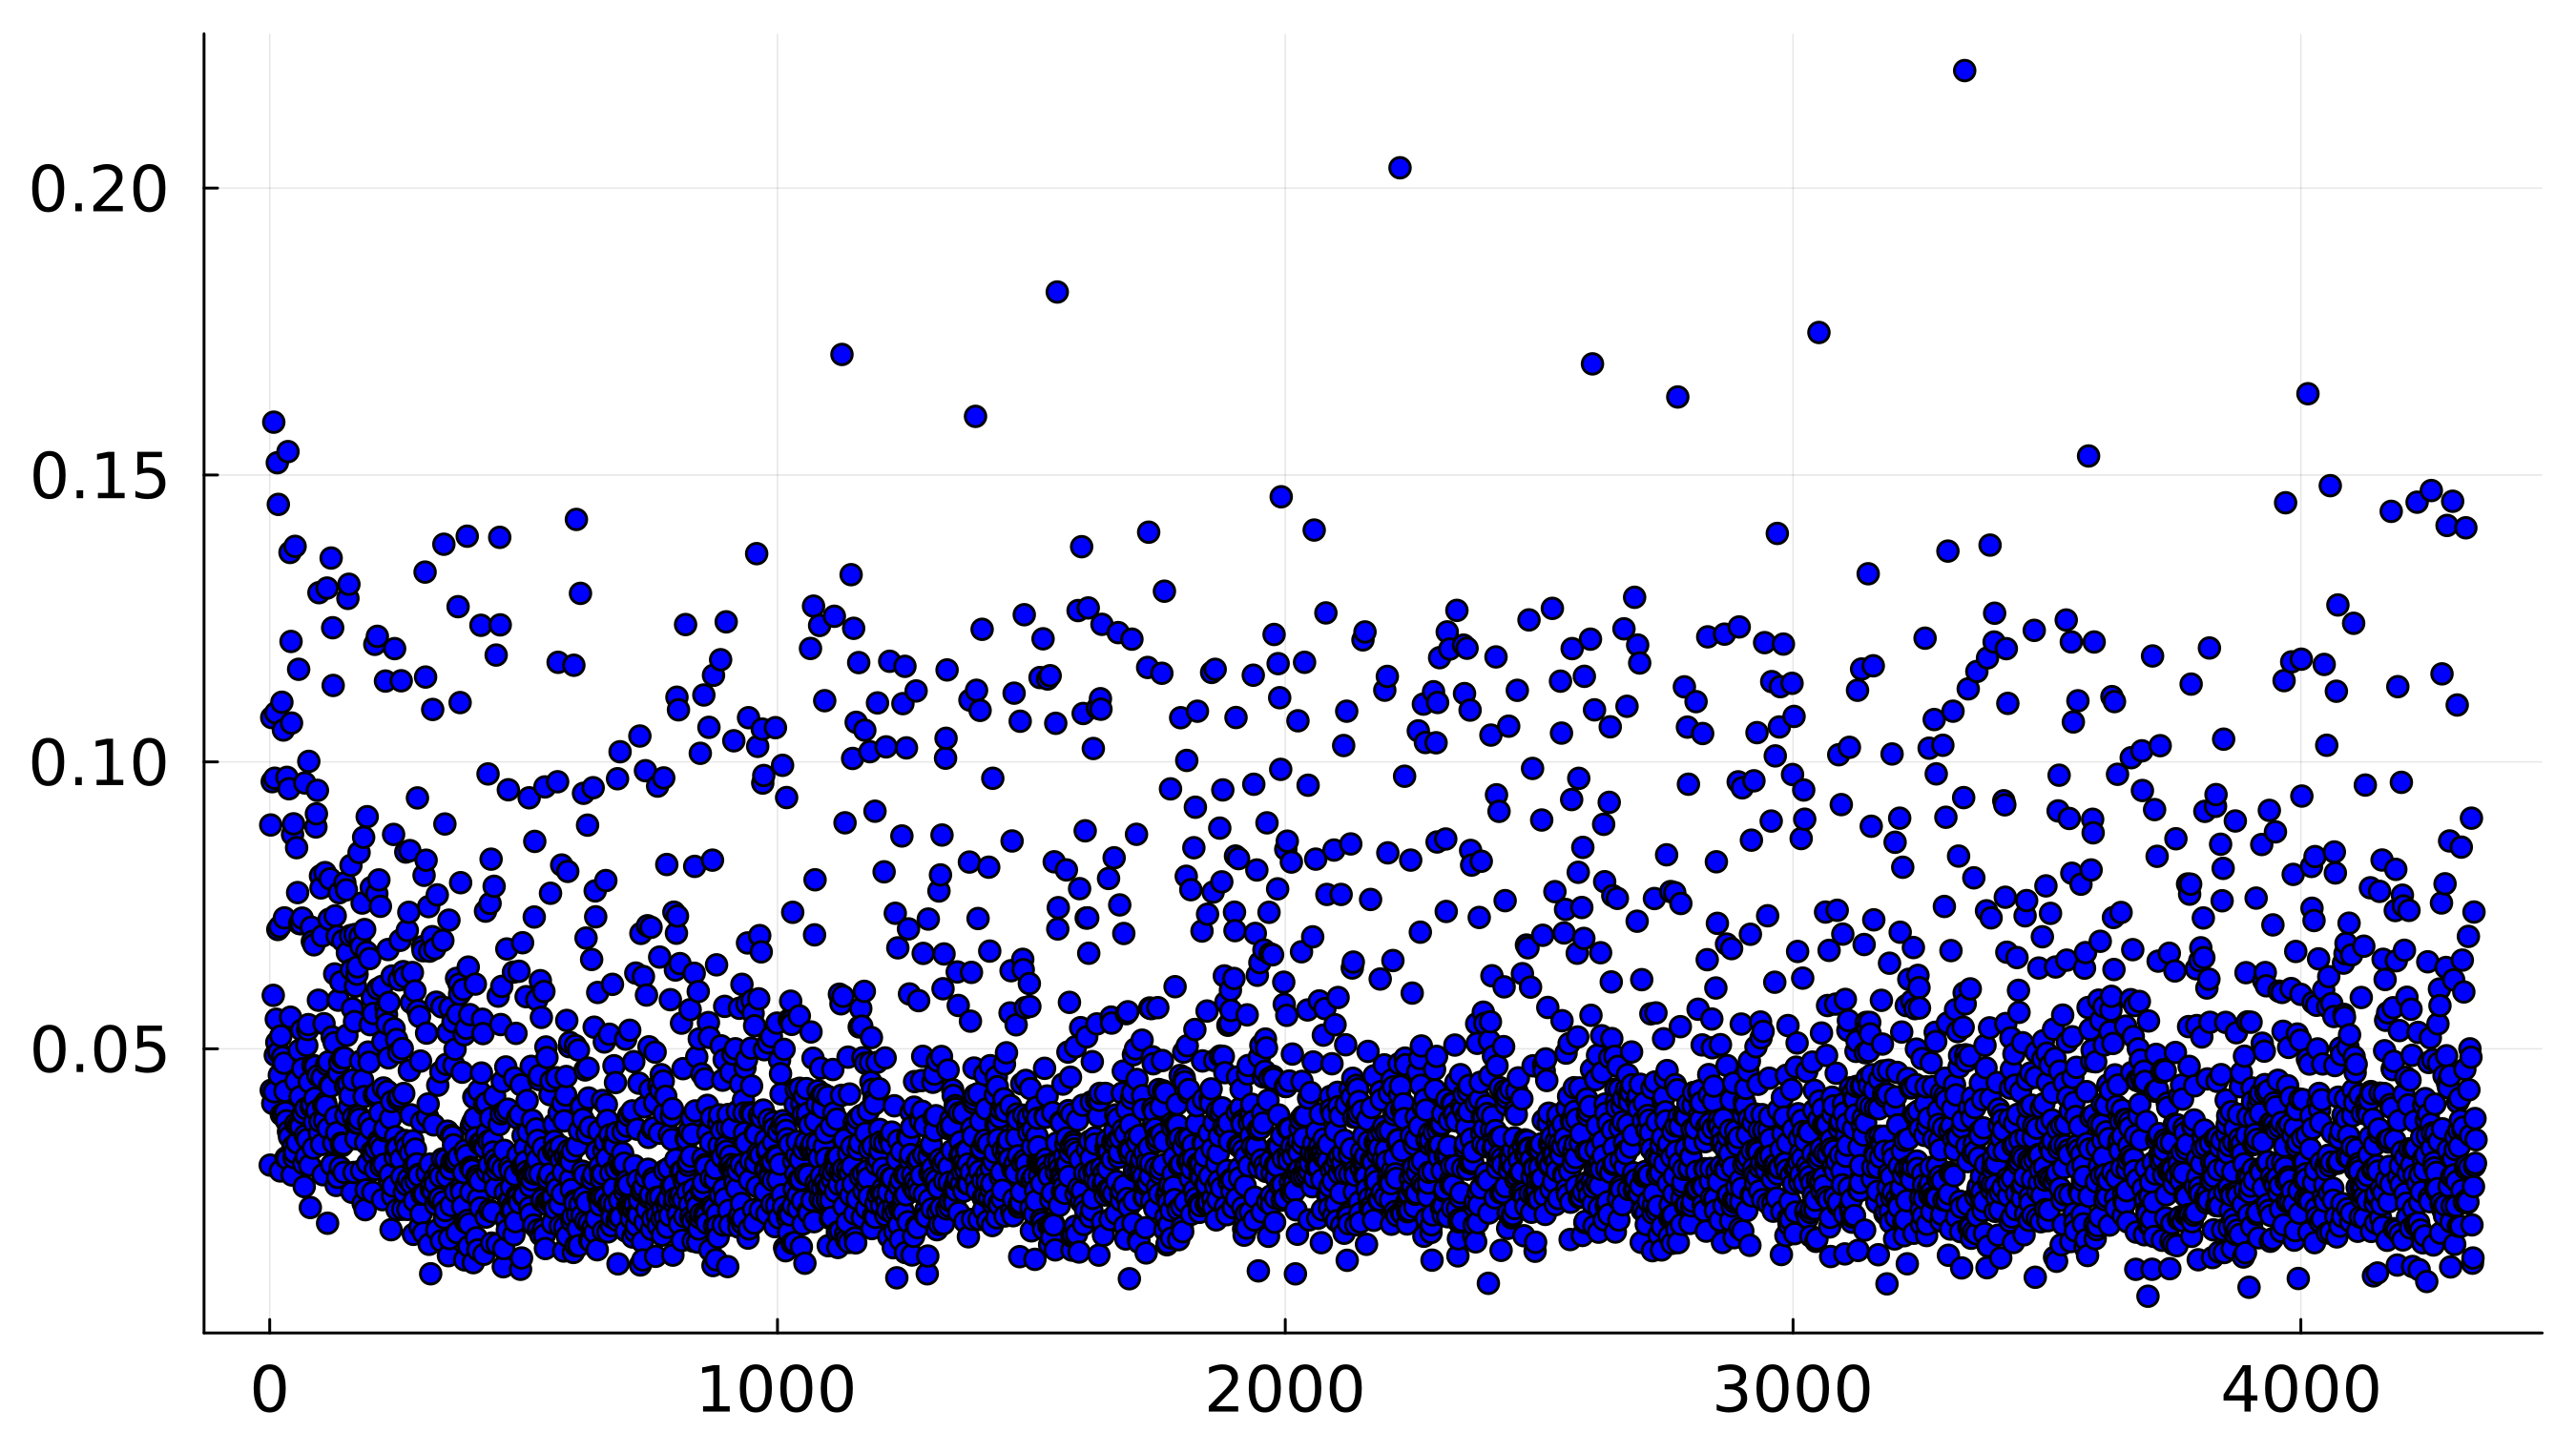
\includegraphics[width=\textwidth]{phalp_bow_rand_learning3}
        \caption{Embeddings using random amino acid vectors, made \textit{via} the bag-of-words embedding method}
        \label{fig:subfig-a2}
    \end{subfigure}
    \hfill
    \begin{subfigure}{0.48\textwidth}
        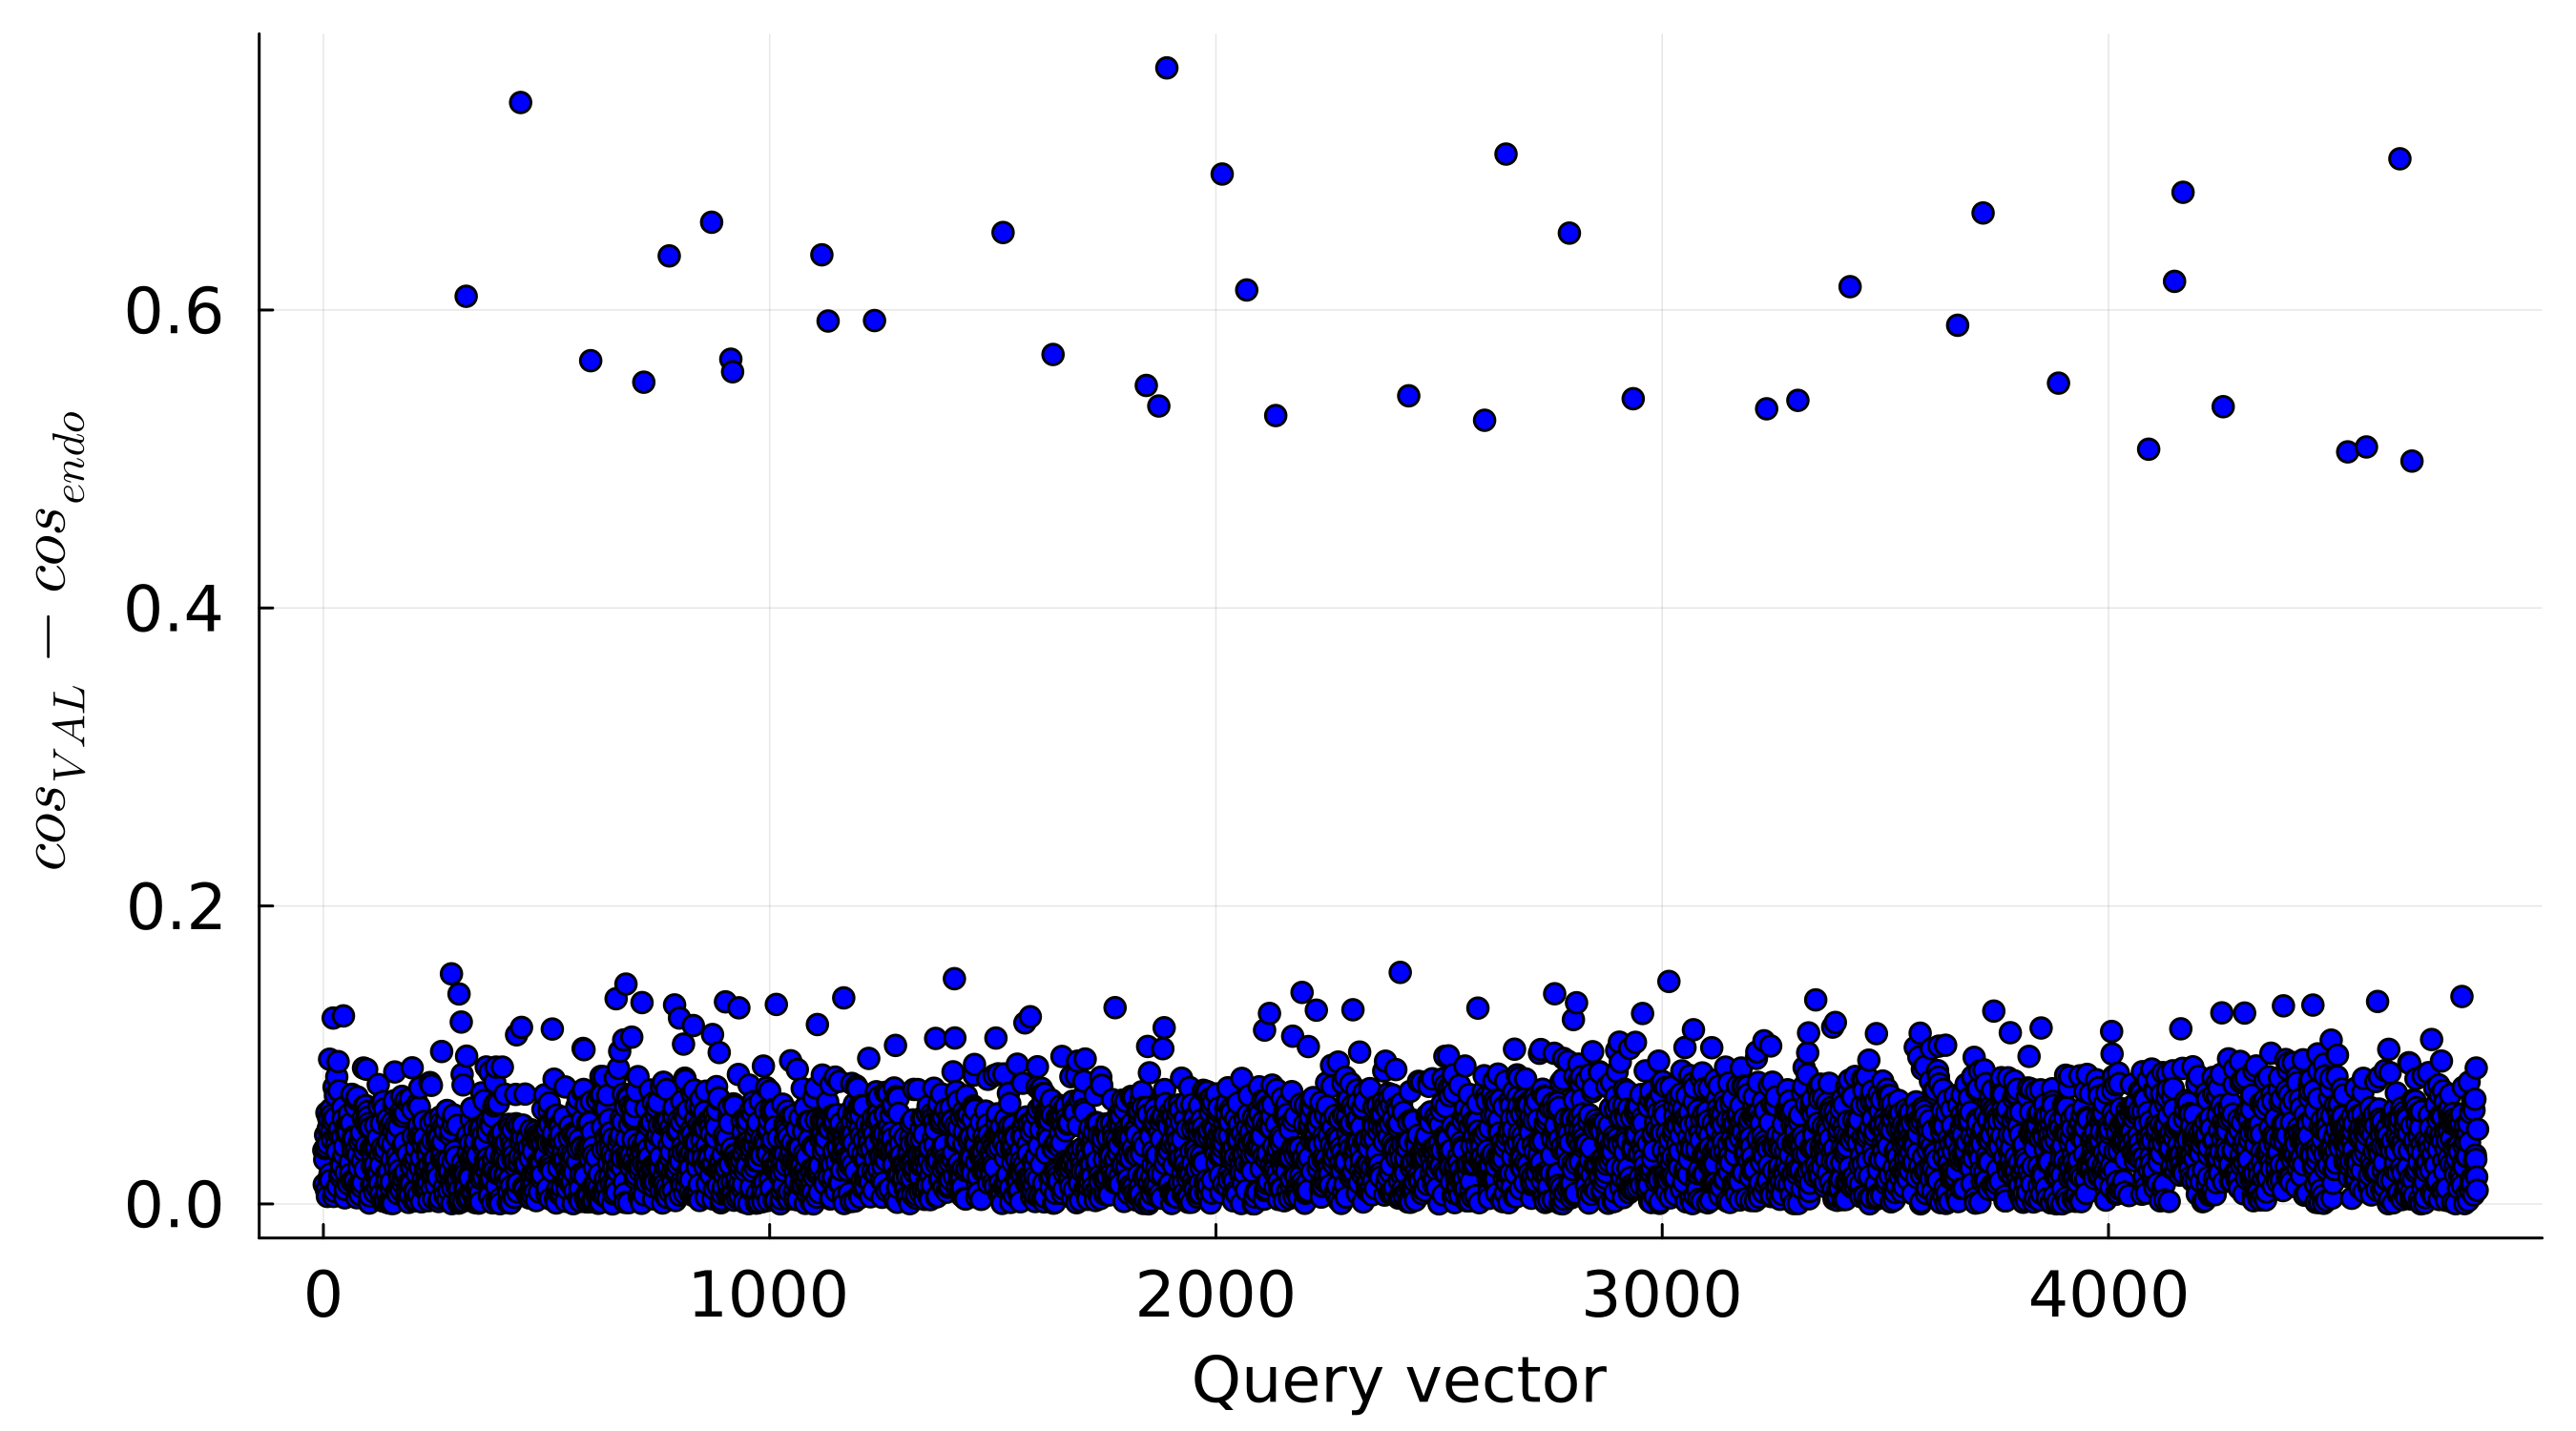
\includegraphics[width=\textwidth]{phalp_bow_esm_learning3}
        \caption{Embeddings using projected ESM-2 amino acid vectors, made \textit{via} the bag-of-words embedding method}
        \label{fig:subfig-b2}
    \end{subfigure}
    
    \begin{subfigure}{0.48\textwidth}
        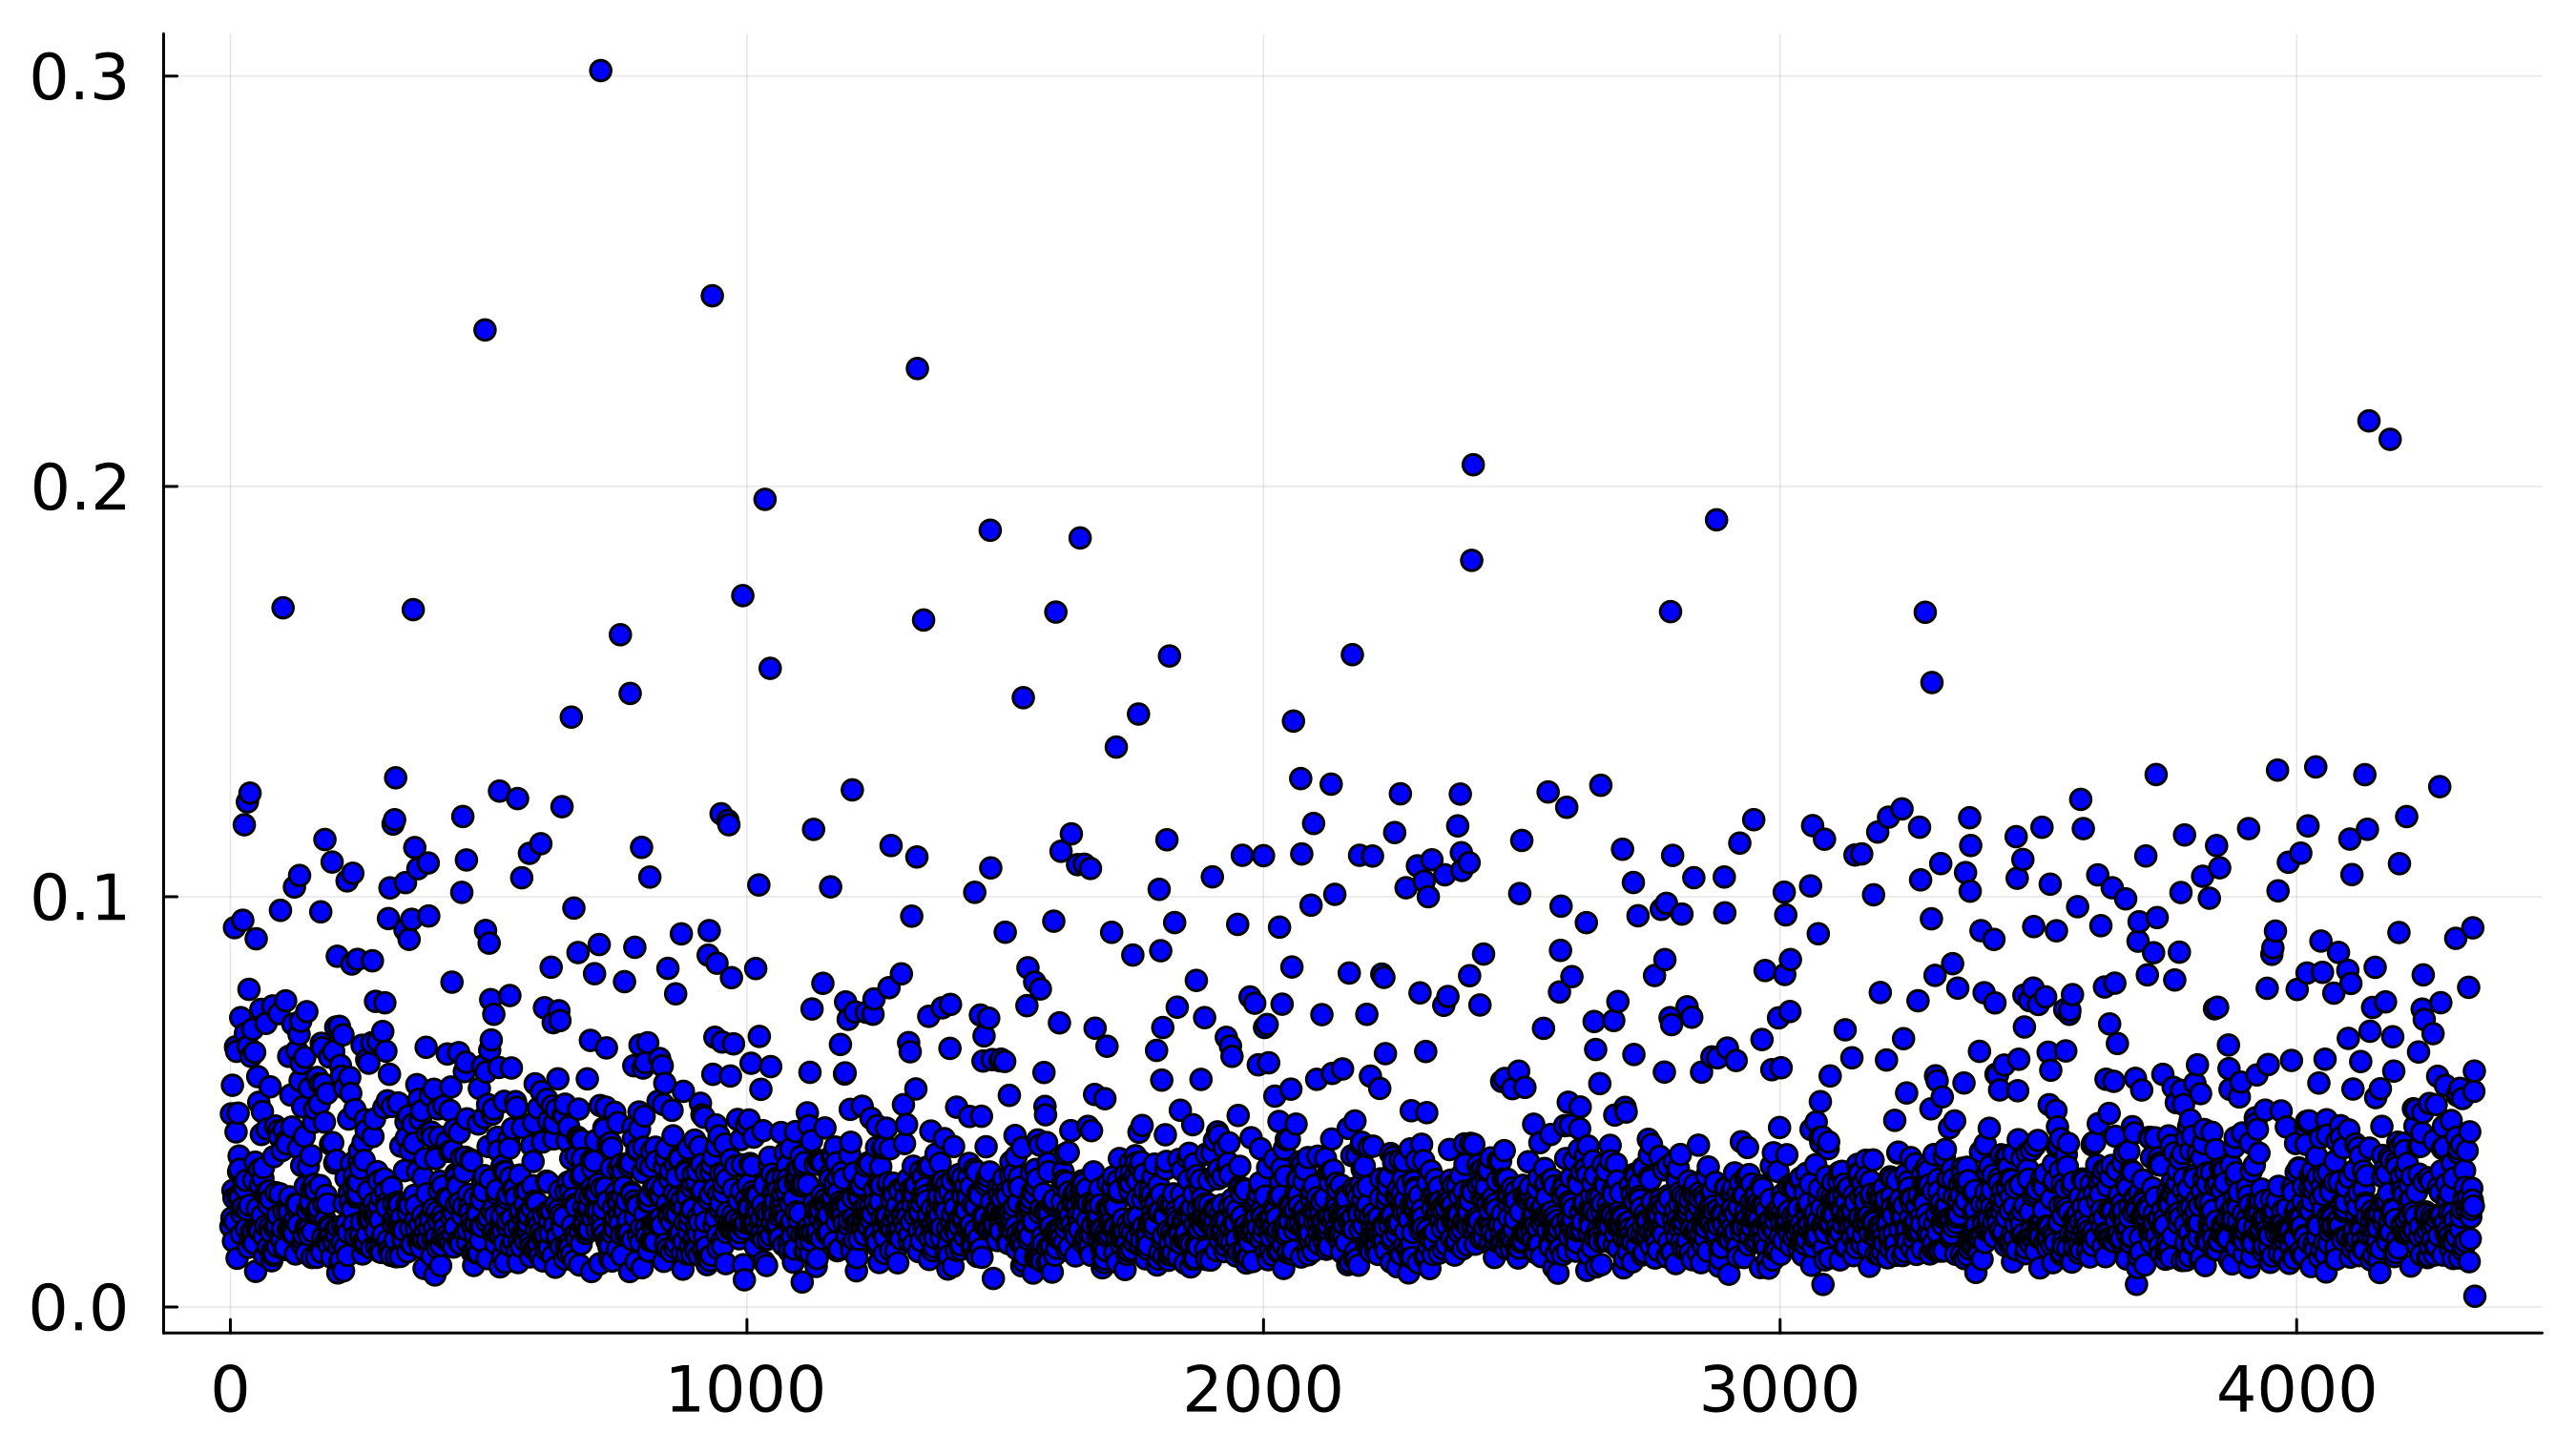
\includegraphics[width=\textwidth]{phalp_cnn_rand_learning3}
        \caption{Embeddings using random amino acid vectors, made \textit{via} the convolutional embedding method}
        \label{fig:subfig-c2}
    \end{subfigure}
    \hfill
    \begin{subfigure}{0.48\textwidth}
        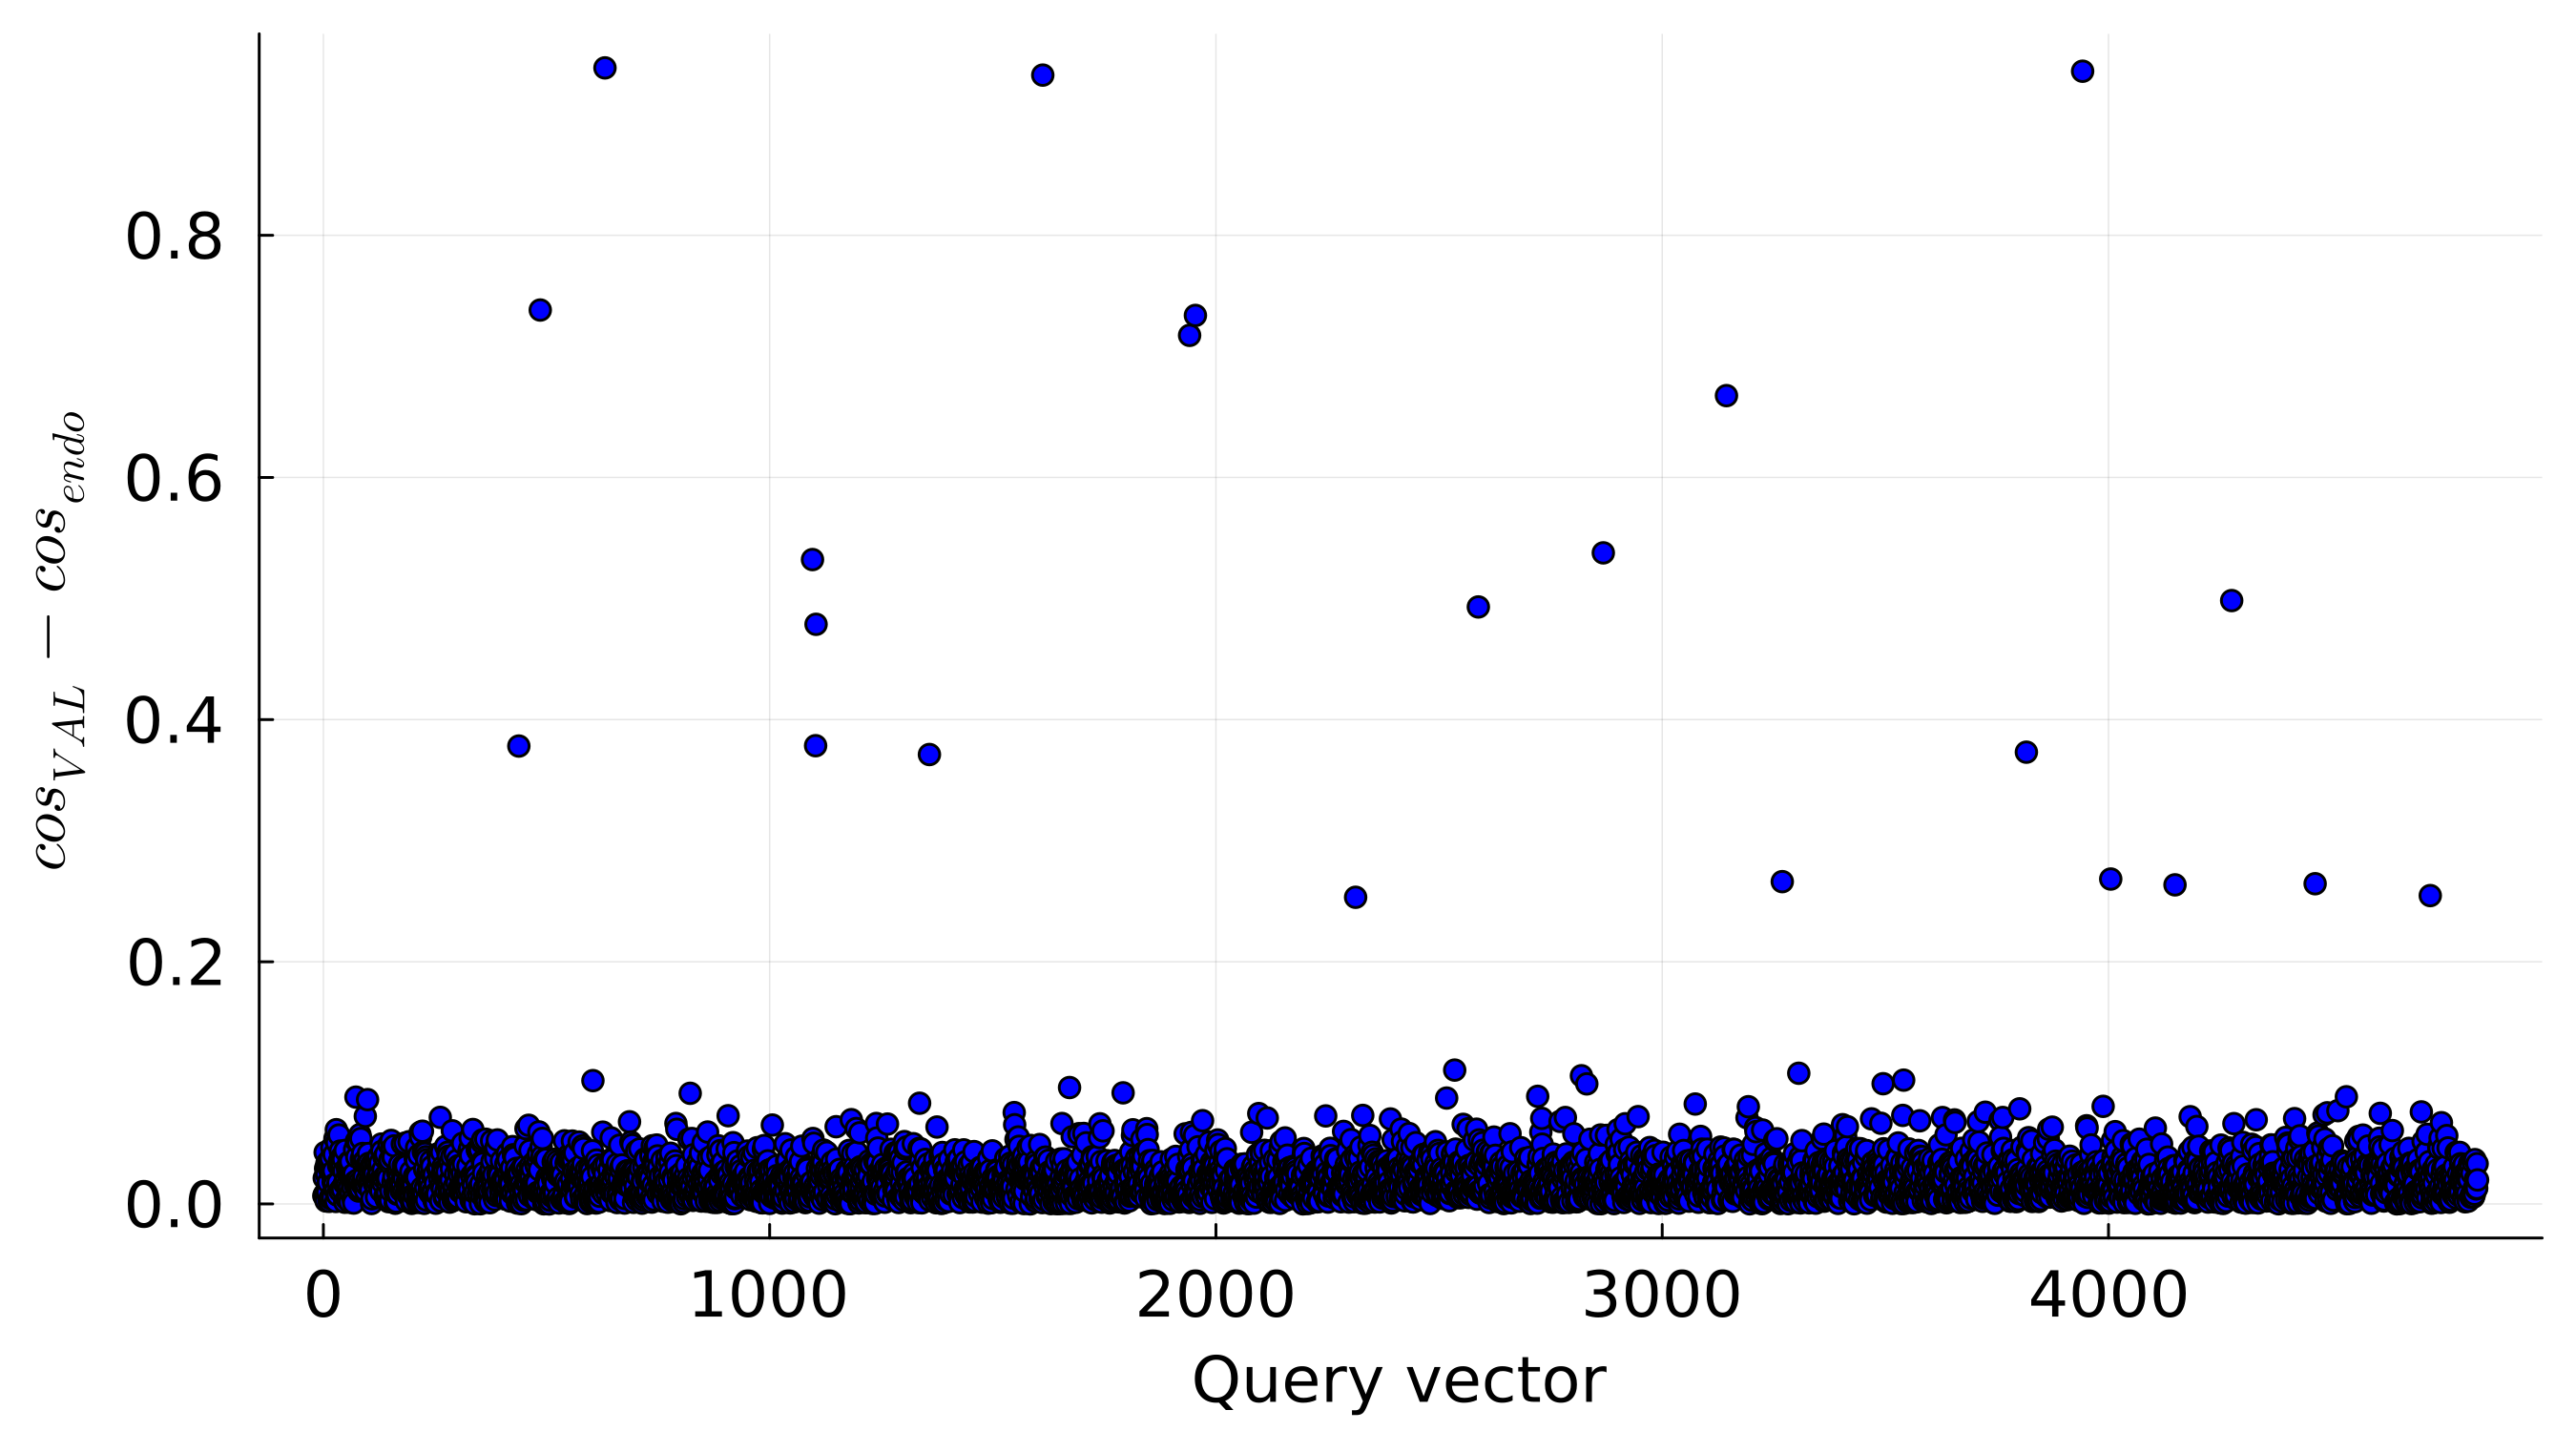
\includegraphics[width=\textwidth]{phalp_cnn_esm_learning3}
        \caption{Embeddings using projected ESM-2 acid vectors, made \textit{via} the convolutional embedding method}
        \label{fig:subfig-d2}
    \end{subfigure}
    \caption{Absolute difference between the cosine similarity of the query vector with the VAL class vector and the cosine similarity of the query vector with the endolysin class vector before the weighted update while following the OnlineHD single-pass training procedure. Trained using hyperdimensional embeddings from all protein sequences in the PhaLP dataset whose types were manually annotated.}
    \label{fig:main2}
\end{figure}

To further research the power of OnlineHD, we aim to monitor its training procedure when applied to the PhaLP dataset. We calculate the absolute difference between the cosine similarities, $cos(V, C_{VAL})$ and $cos(V, C_{endo})$, as described in equations 4.3 and 4.4. By observing this metric, we can gain insights into the behavior of the hyperdimensional vectors in the OnlineHD model during training. A possibility to expect is that the difference in cosine similarities increases throughout the training procedure as the model learns to differentiate the two classes. However, these differences don't increase noticeably in this case as shown in Figure~\ref{fig:main2}.

\begin{figure}[ht!]
    \centering
    \begin{subfigure}{0.48\textwidth}
        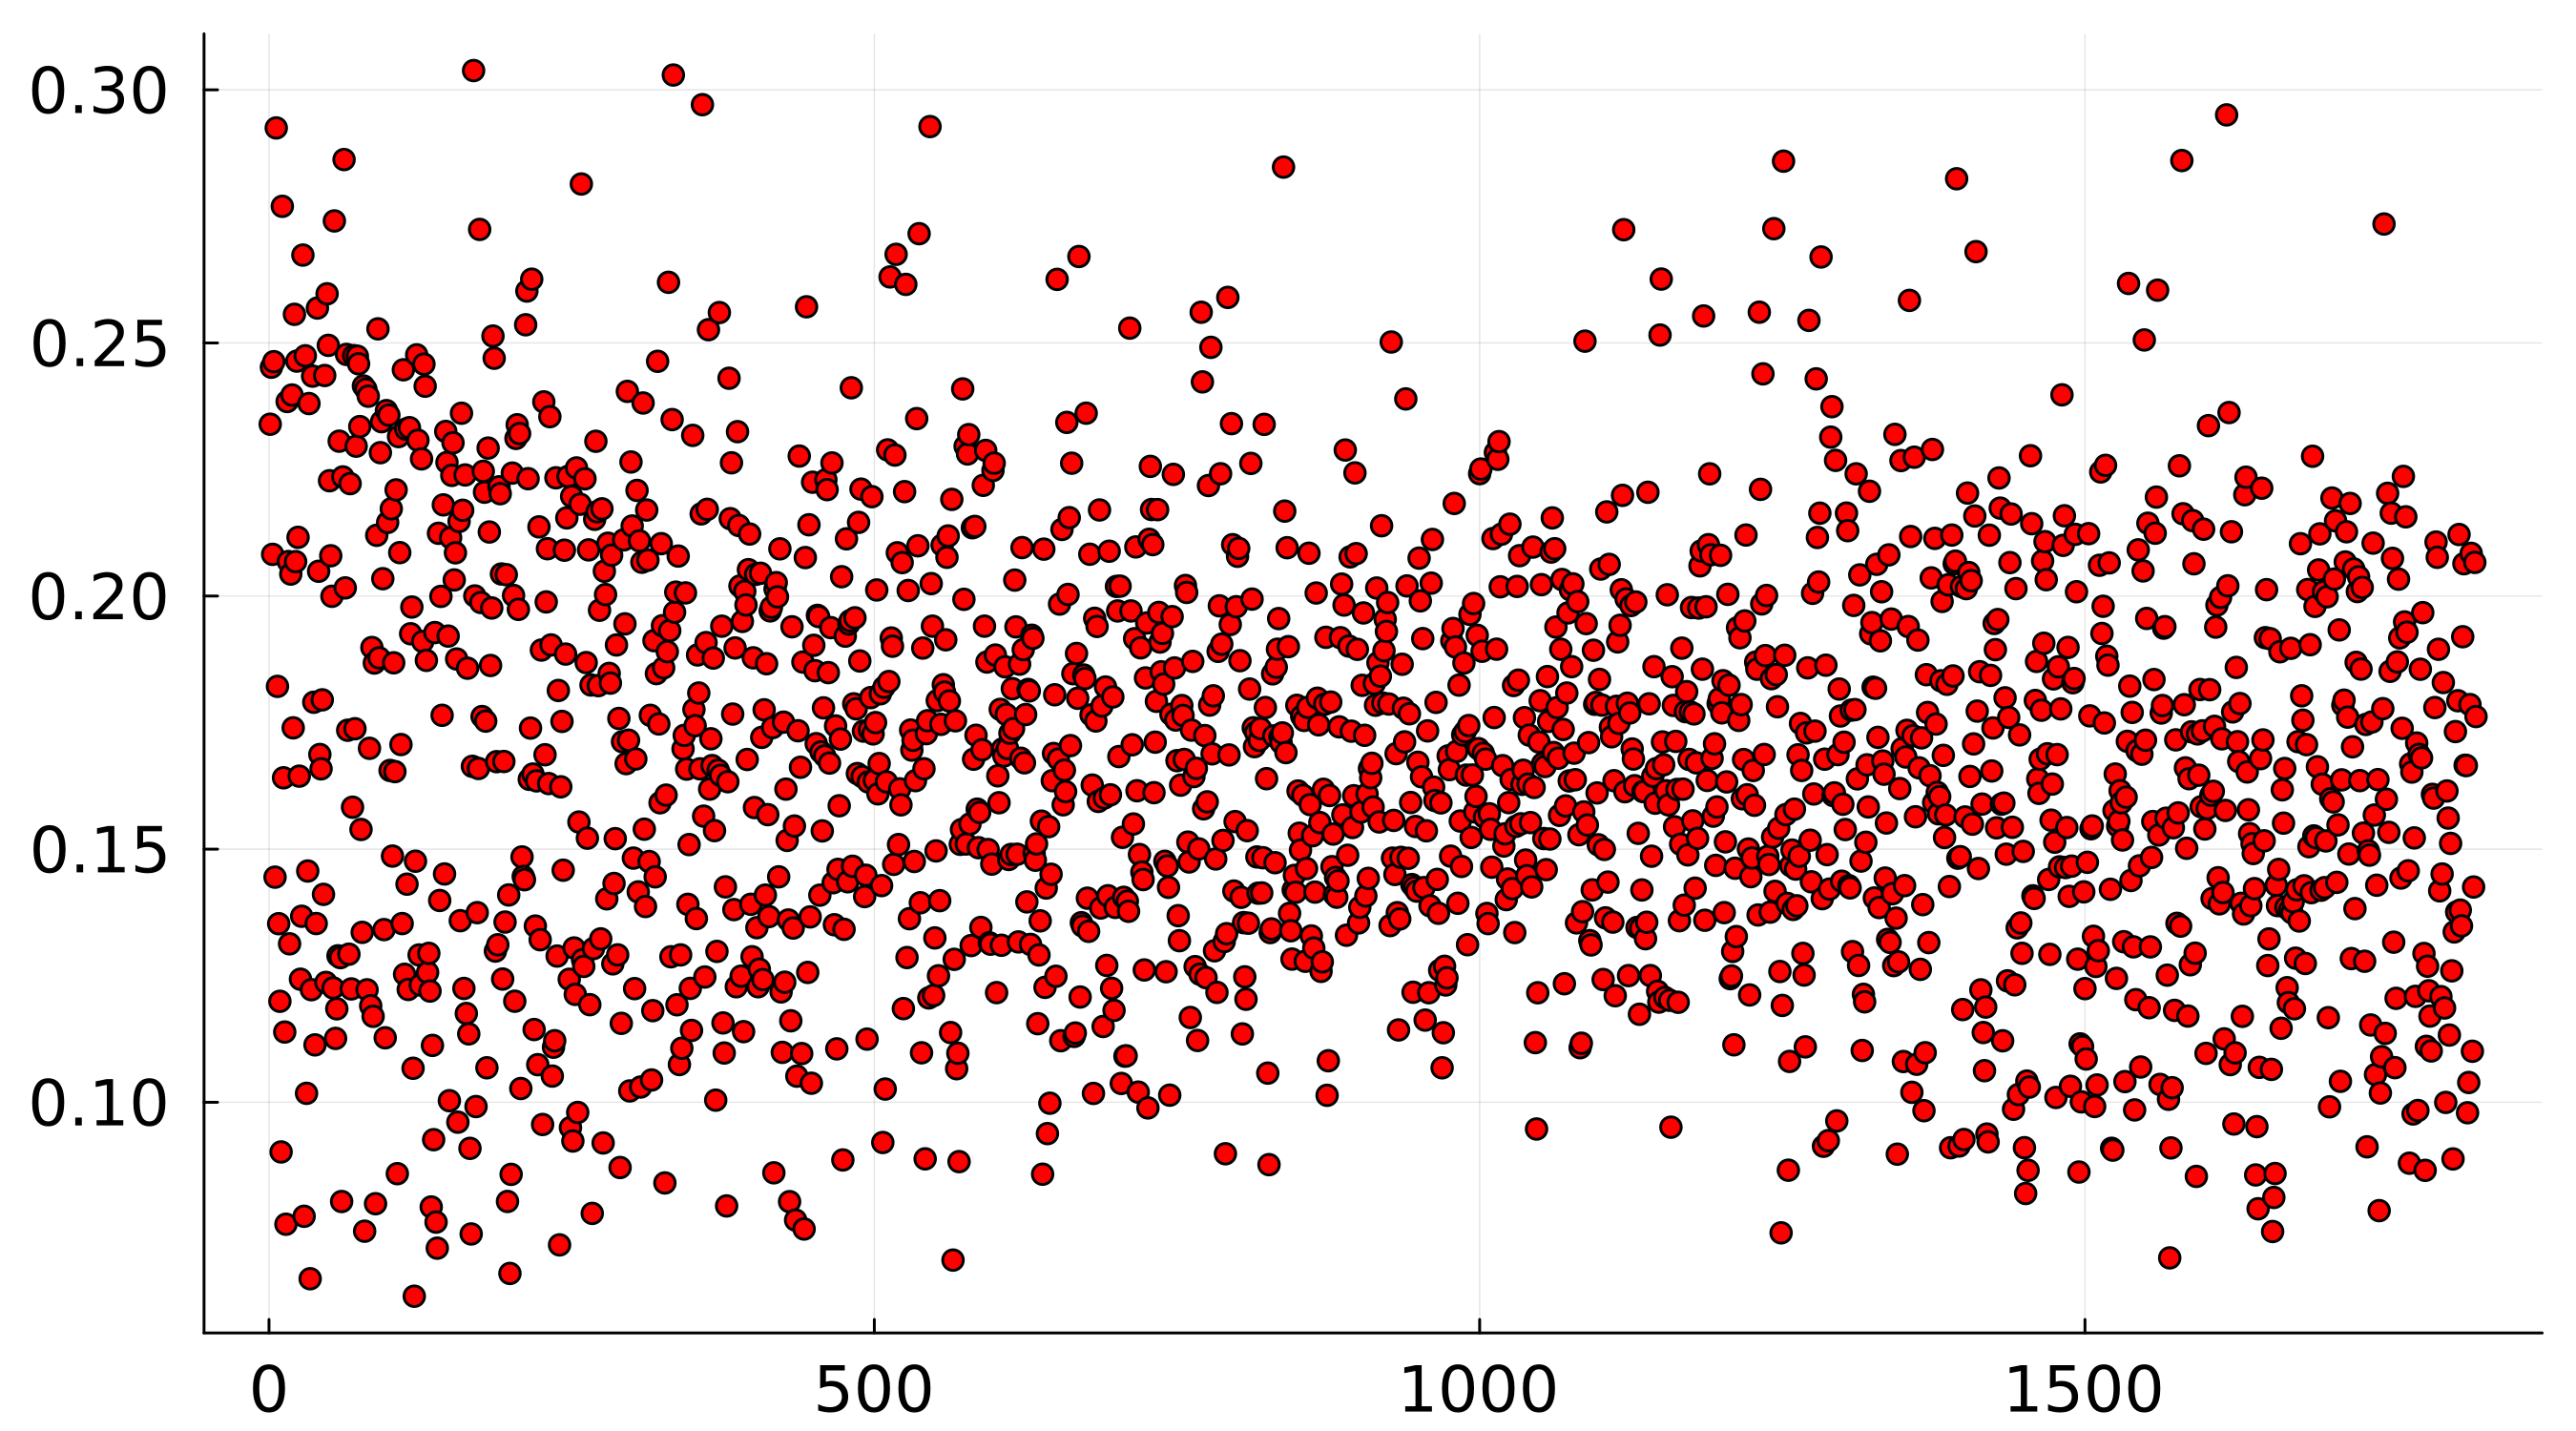
\includegraphics[width=\textwidth]{phalp_bow_rand_learningV}
        \caption{VALs embedded using random amino acid vectors \textit{via} the bag-of-words method}
        \label{fig:subfig-a}
    \end{subfigure}
    \hfill
    \begin{subfigure}{0.48\textwidth}
        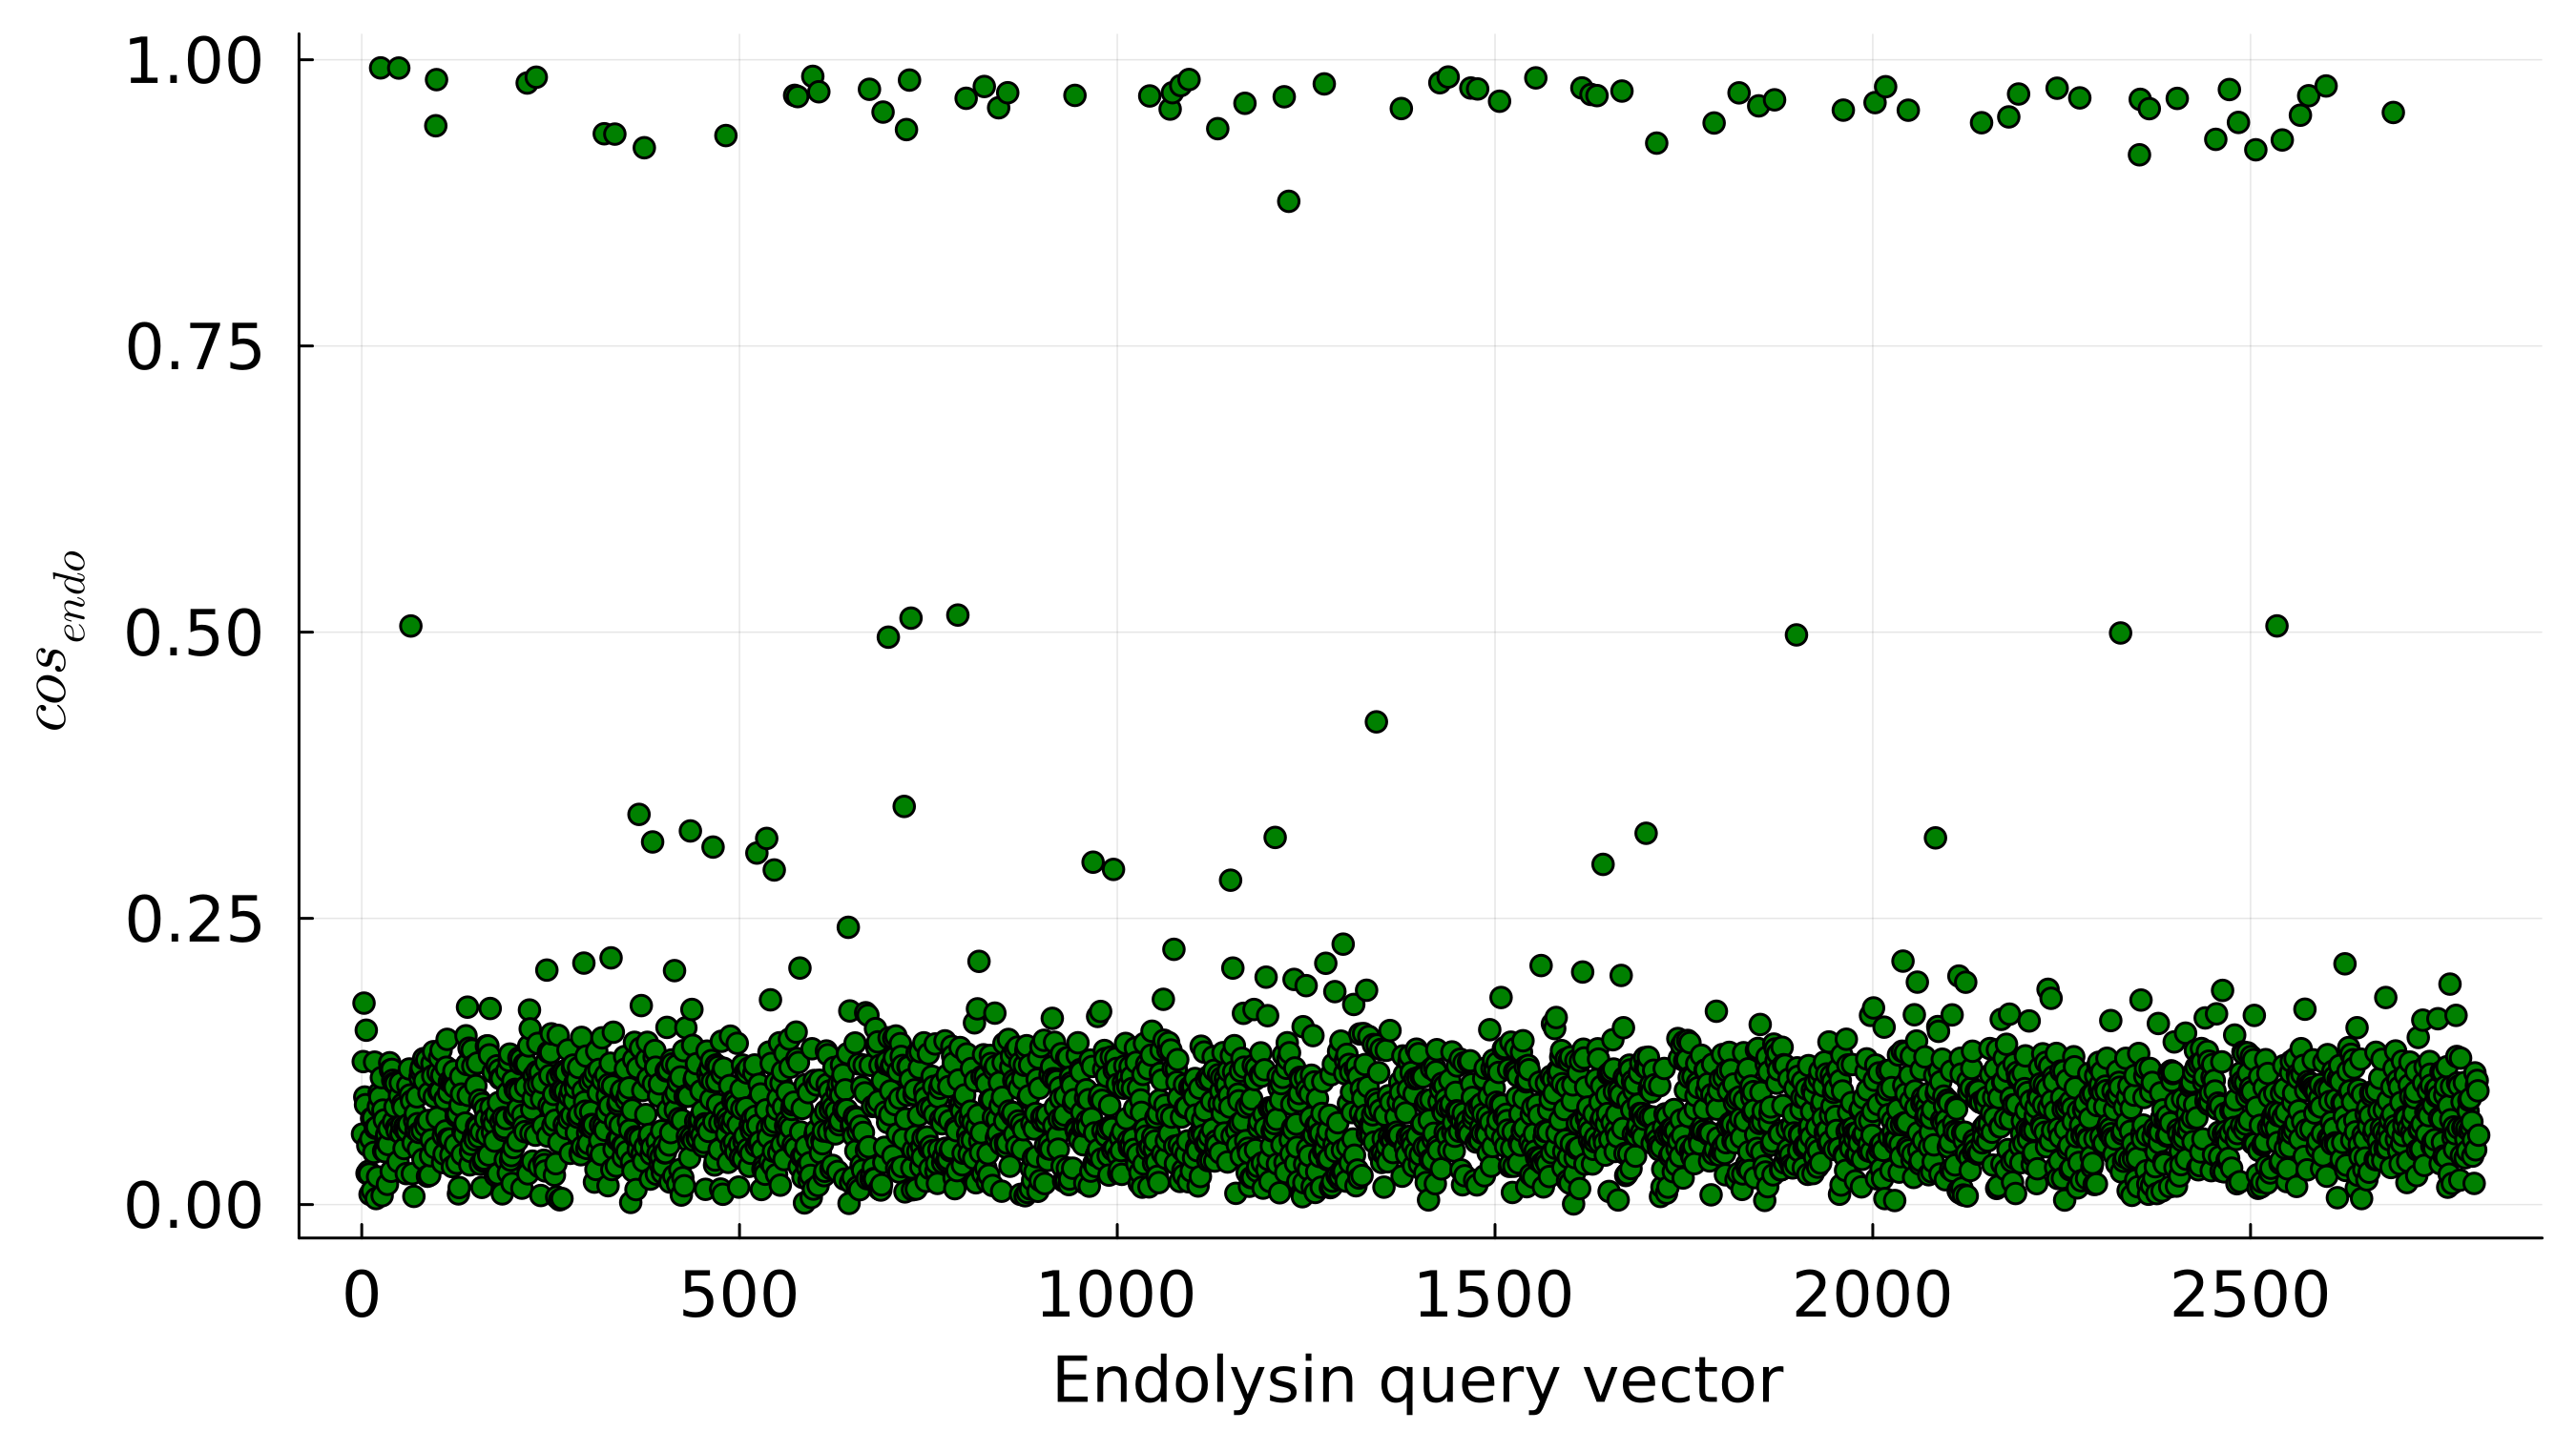
\includegraphics[width=\textwidth]{phalp_bow_rand_learningE}
        \caption{Endolysins embedded using random amino acid vectors \textit{via} the bag-of-words embedding method}
        \label{fig:subfig-b}
    \end{subfigure}
    
    \begin{subfigure}{0.48\textwidth}
        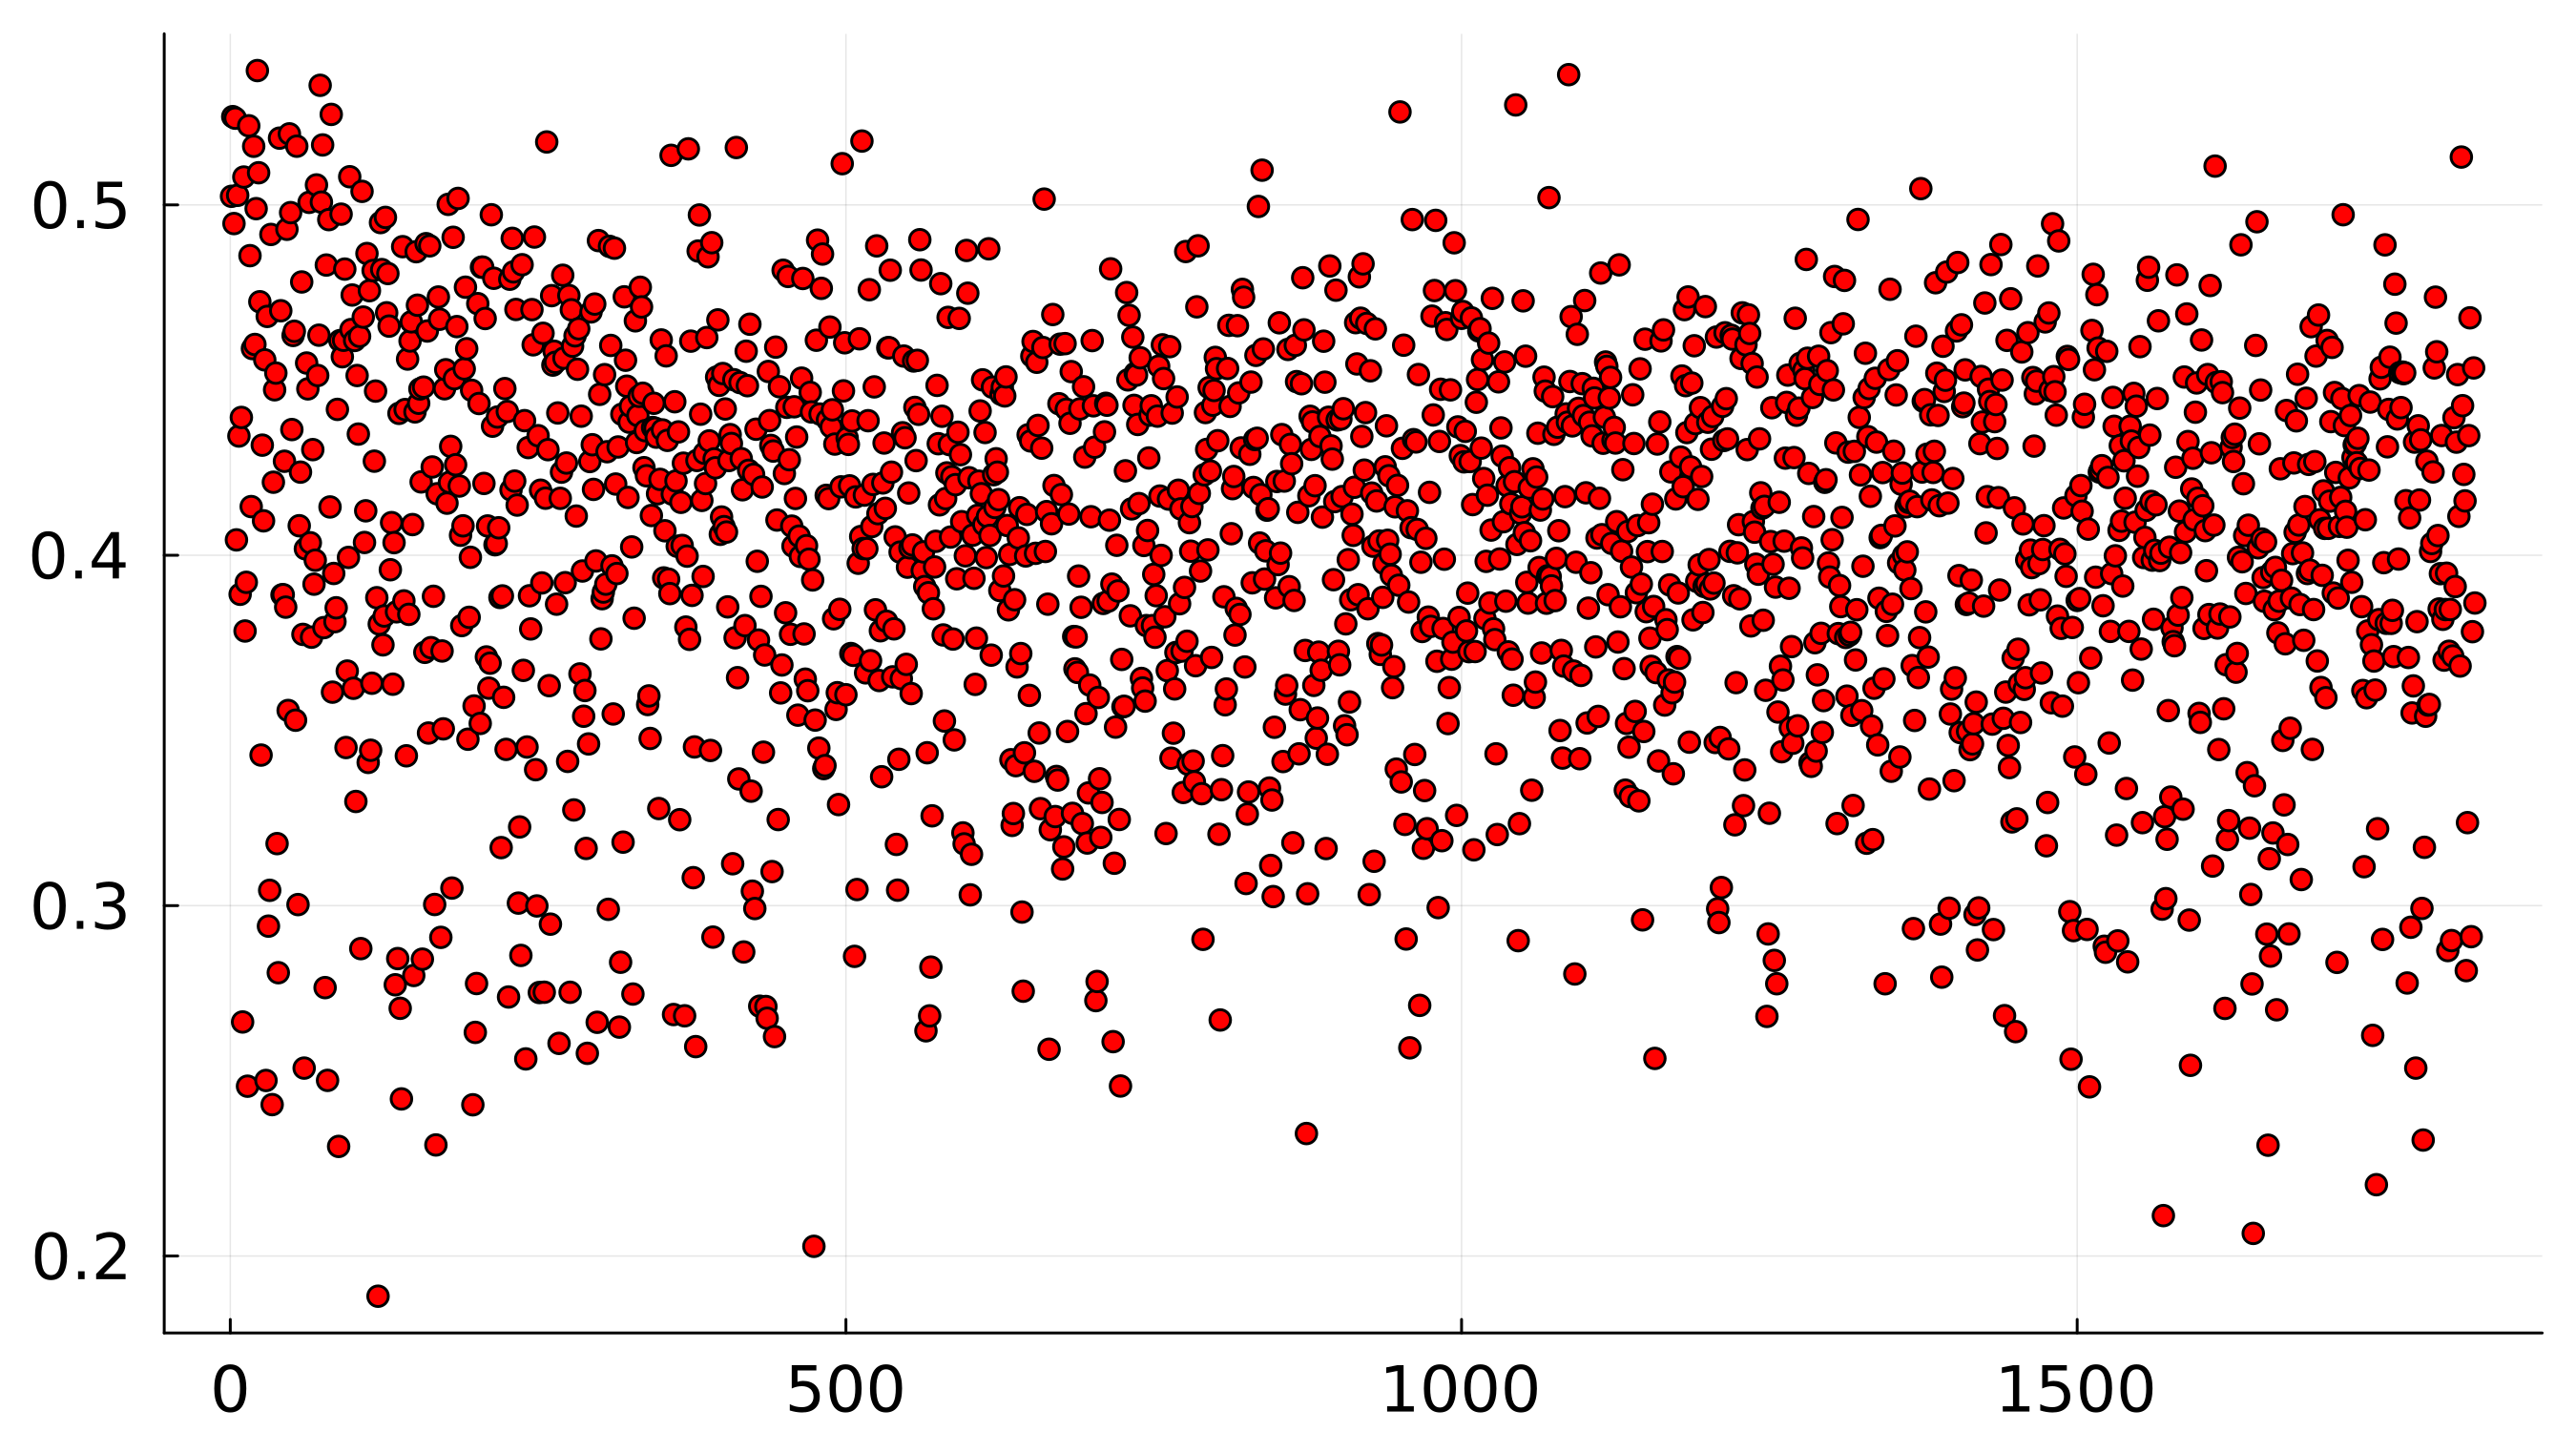
\includegraphics[width=\textwidth]{phalp_bow_esm_learningV}
        \caption{VALs embedded using projected ESM-2 amino acid vectors \textit{via} the bag-of-words embedding method}
        \label{fig:subfig-c}
    \end{subfigure}
    \hfill
    \begin{subfigure}{0.48\textwidth}
        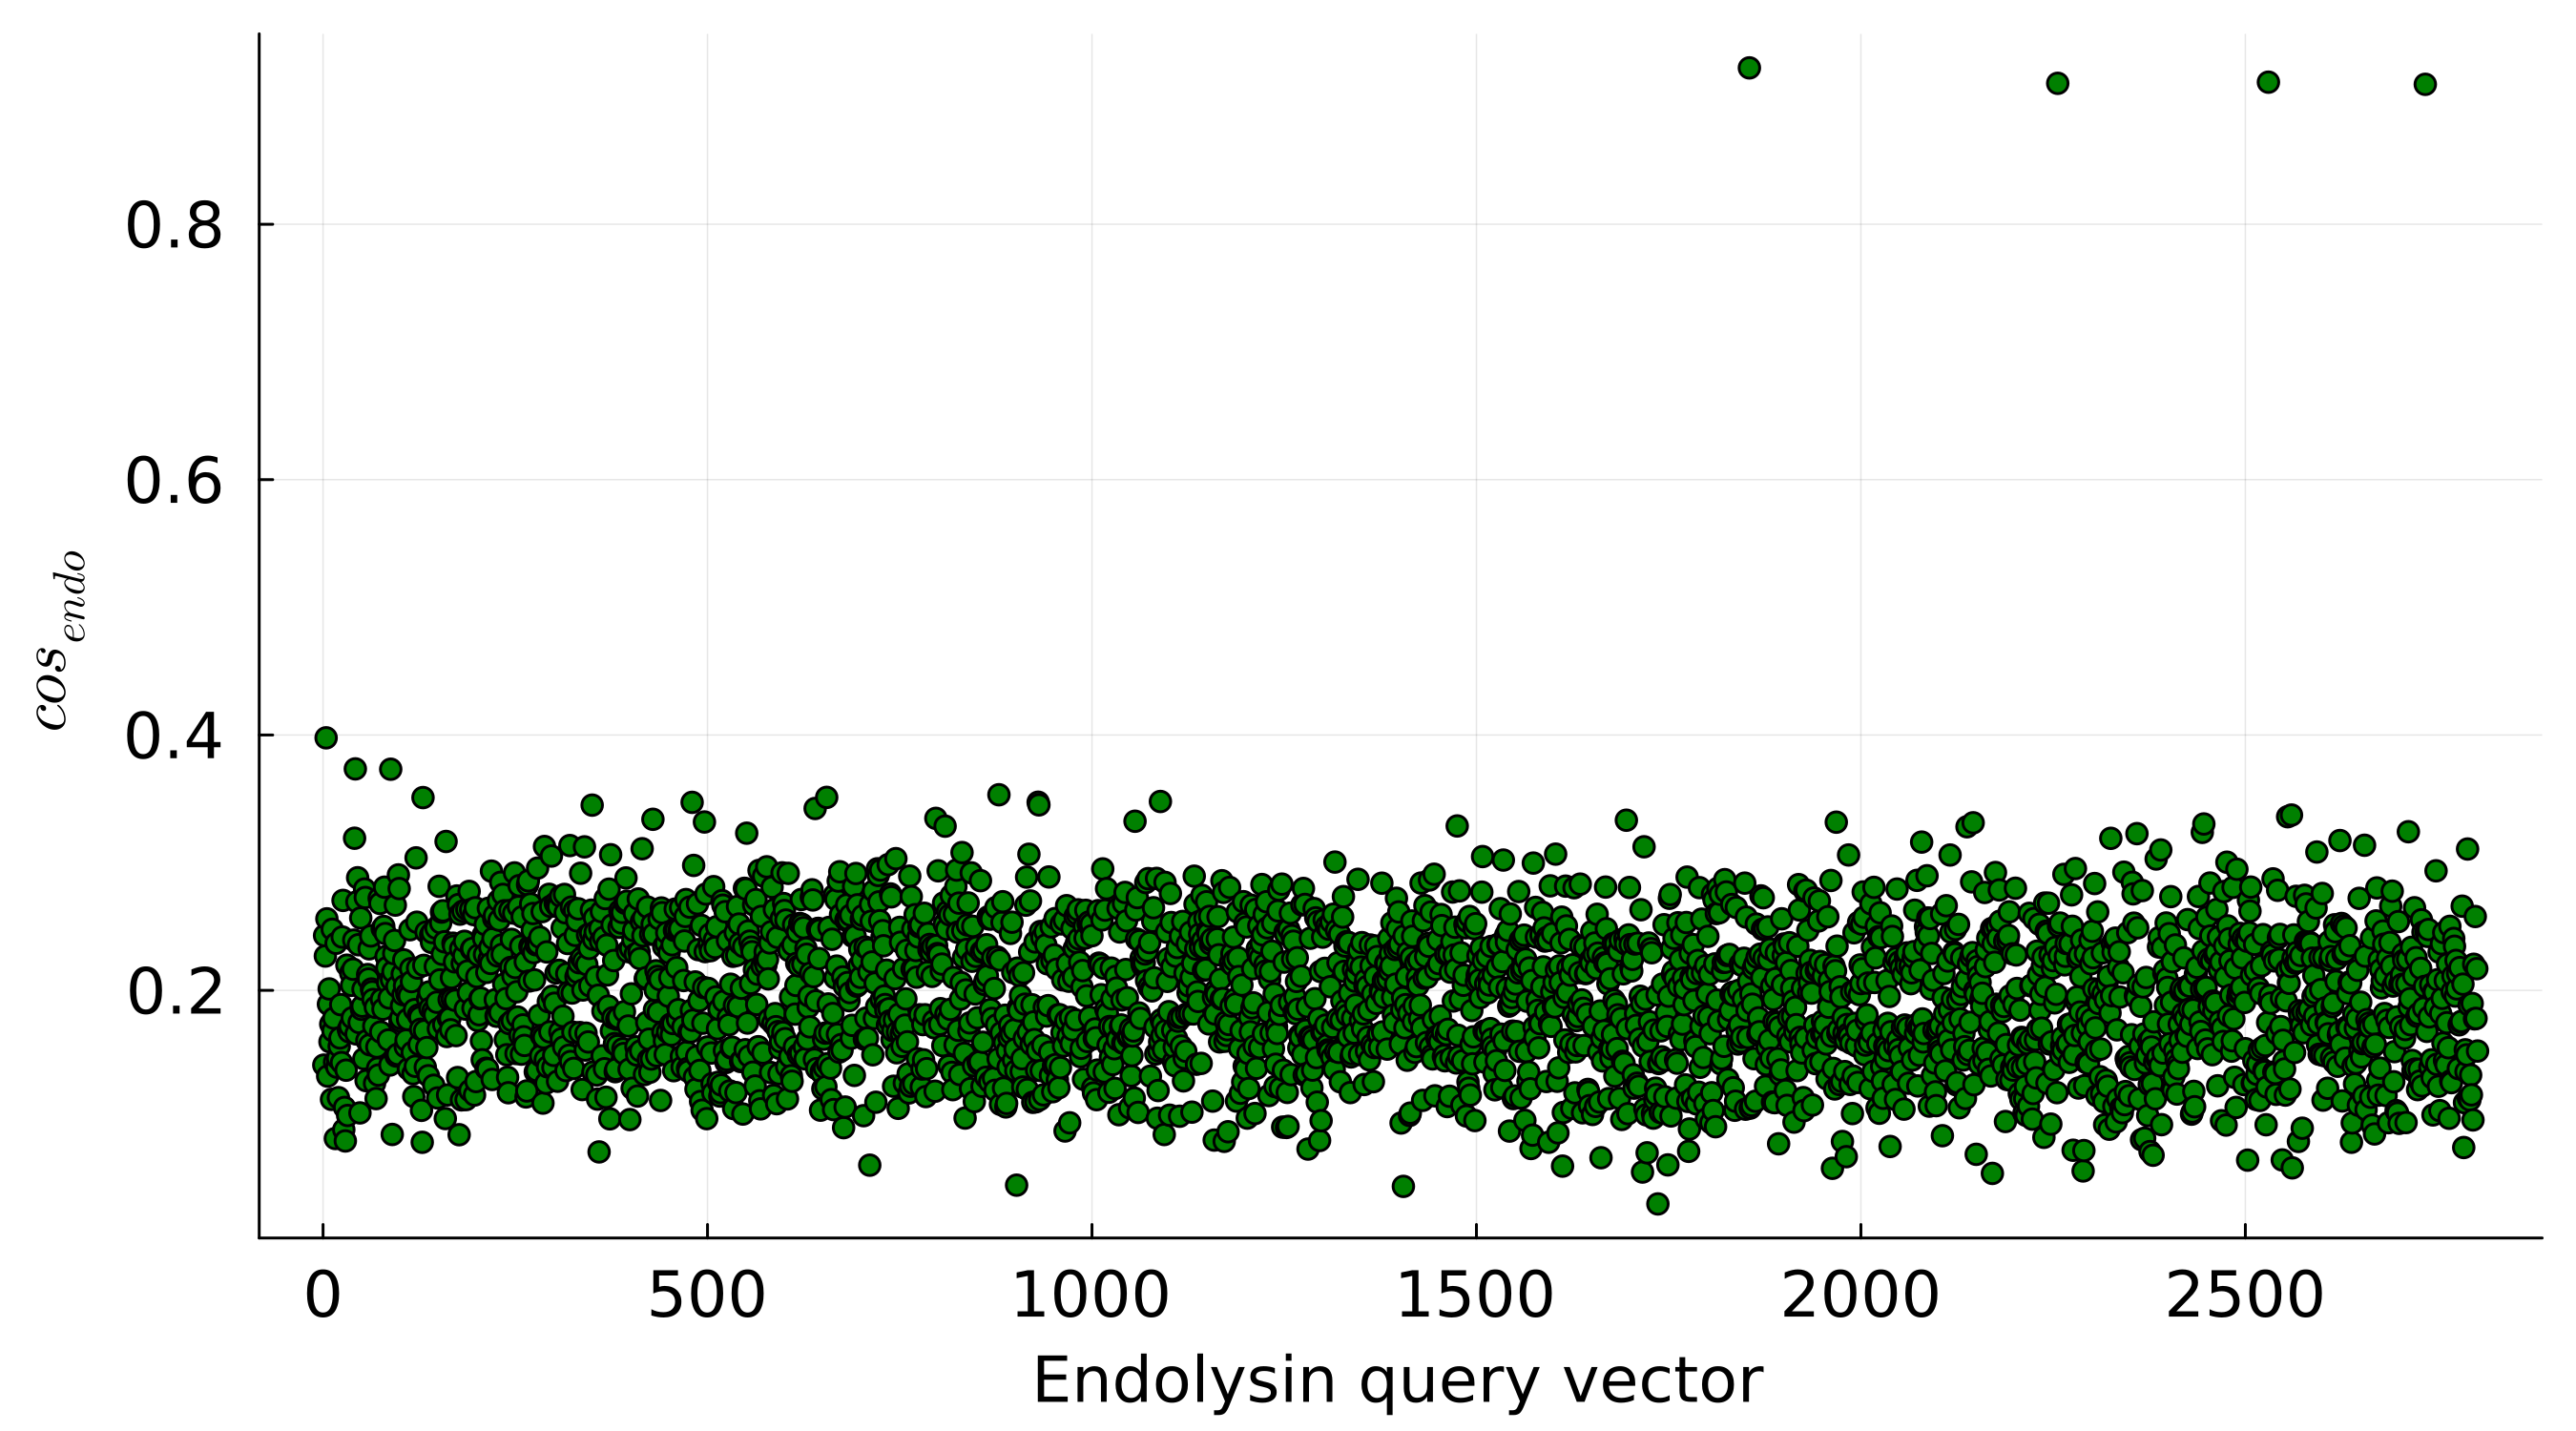
\includegraphics[width=\textwidth]{phalp_bow_esm_learningE}
        \caption{Endolysins embedded using projected ESM-2 amino acid vectors \textit{via} the bag-of-words embedding method}
        \label{fig:subfig-d}
    \end{subfigure}
    
    \begin{subfigure}{0.48\textwidth}
        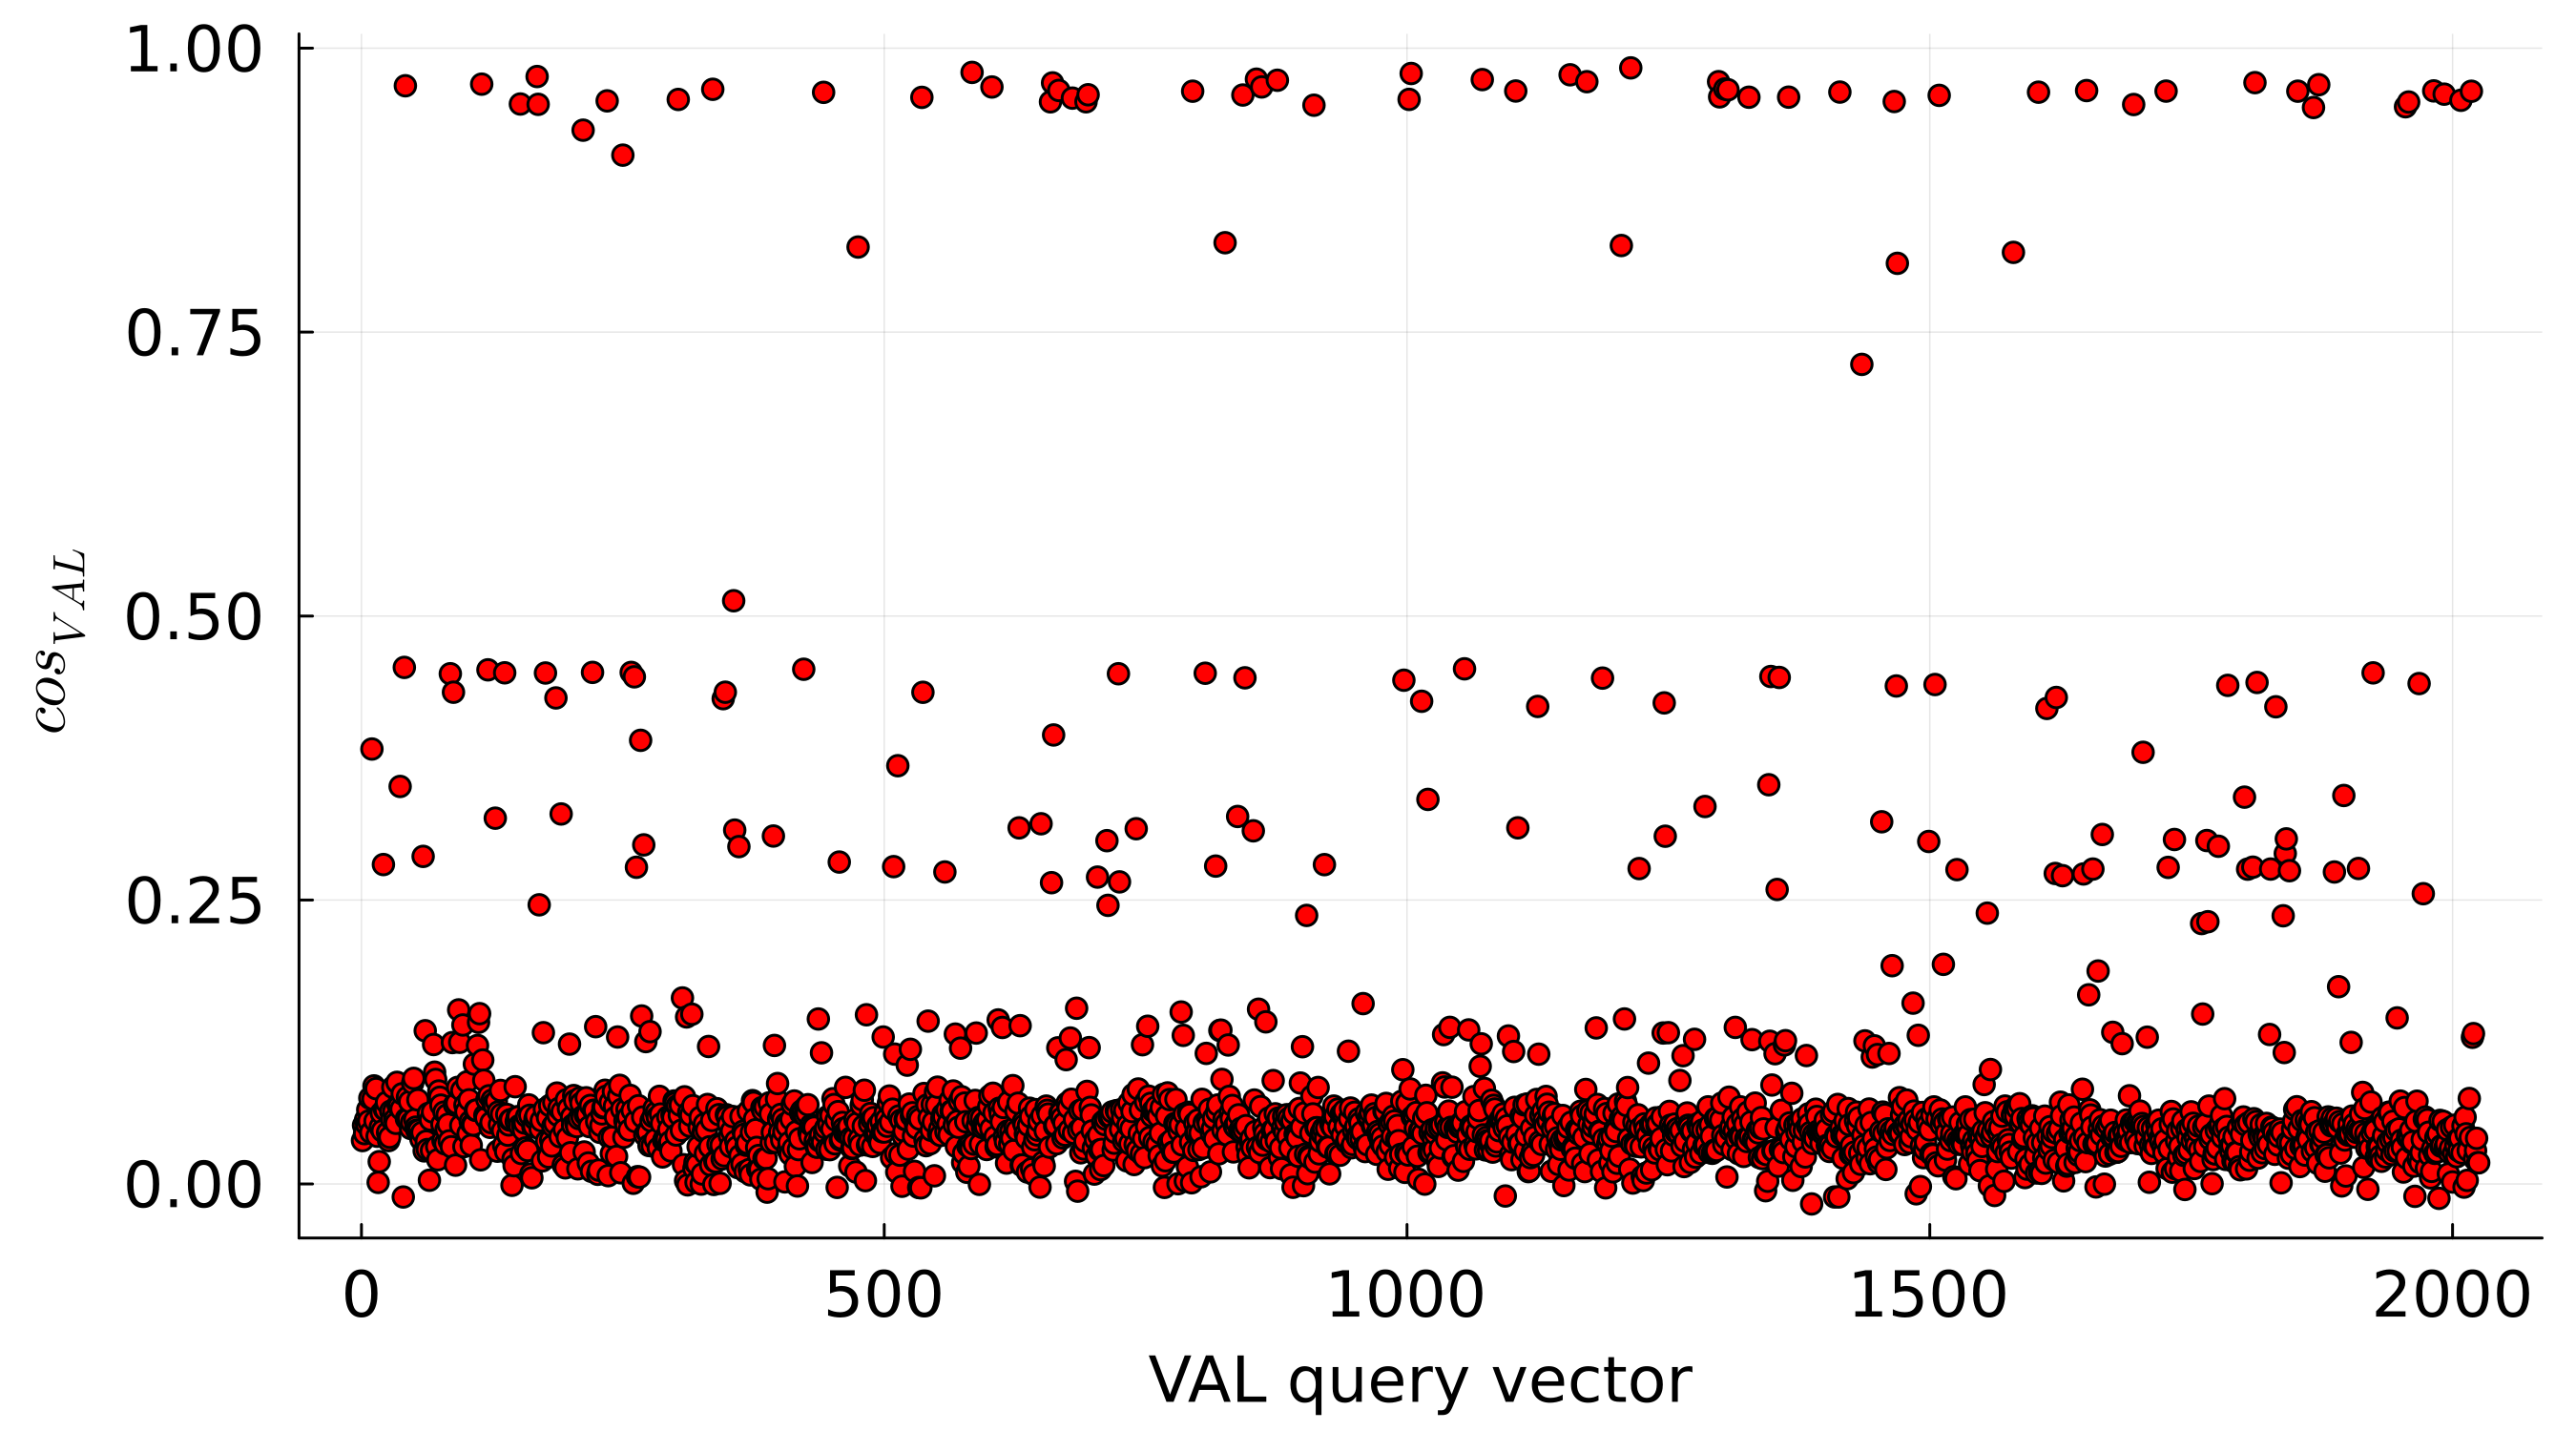
\includegraphics[width=\textwidth]{phalp_cnn_rand_learningV}
        \caption{VALs embedded using using random amino acid vectors \textit{via} the convolutional embedding method}
        \label{fig:subfig-e}
    \end{subfigure}
    \hfill
    \begin{subfigure}{0.48\textwidth}
        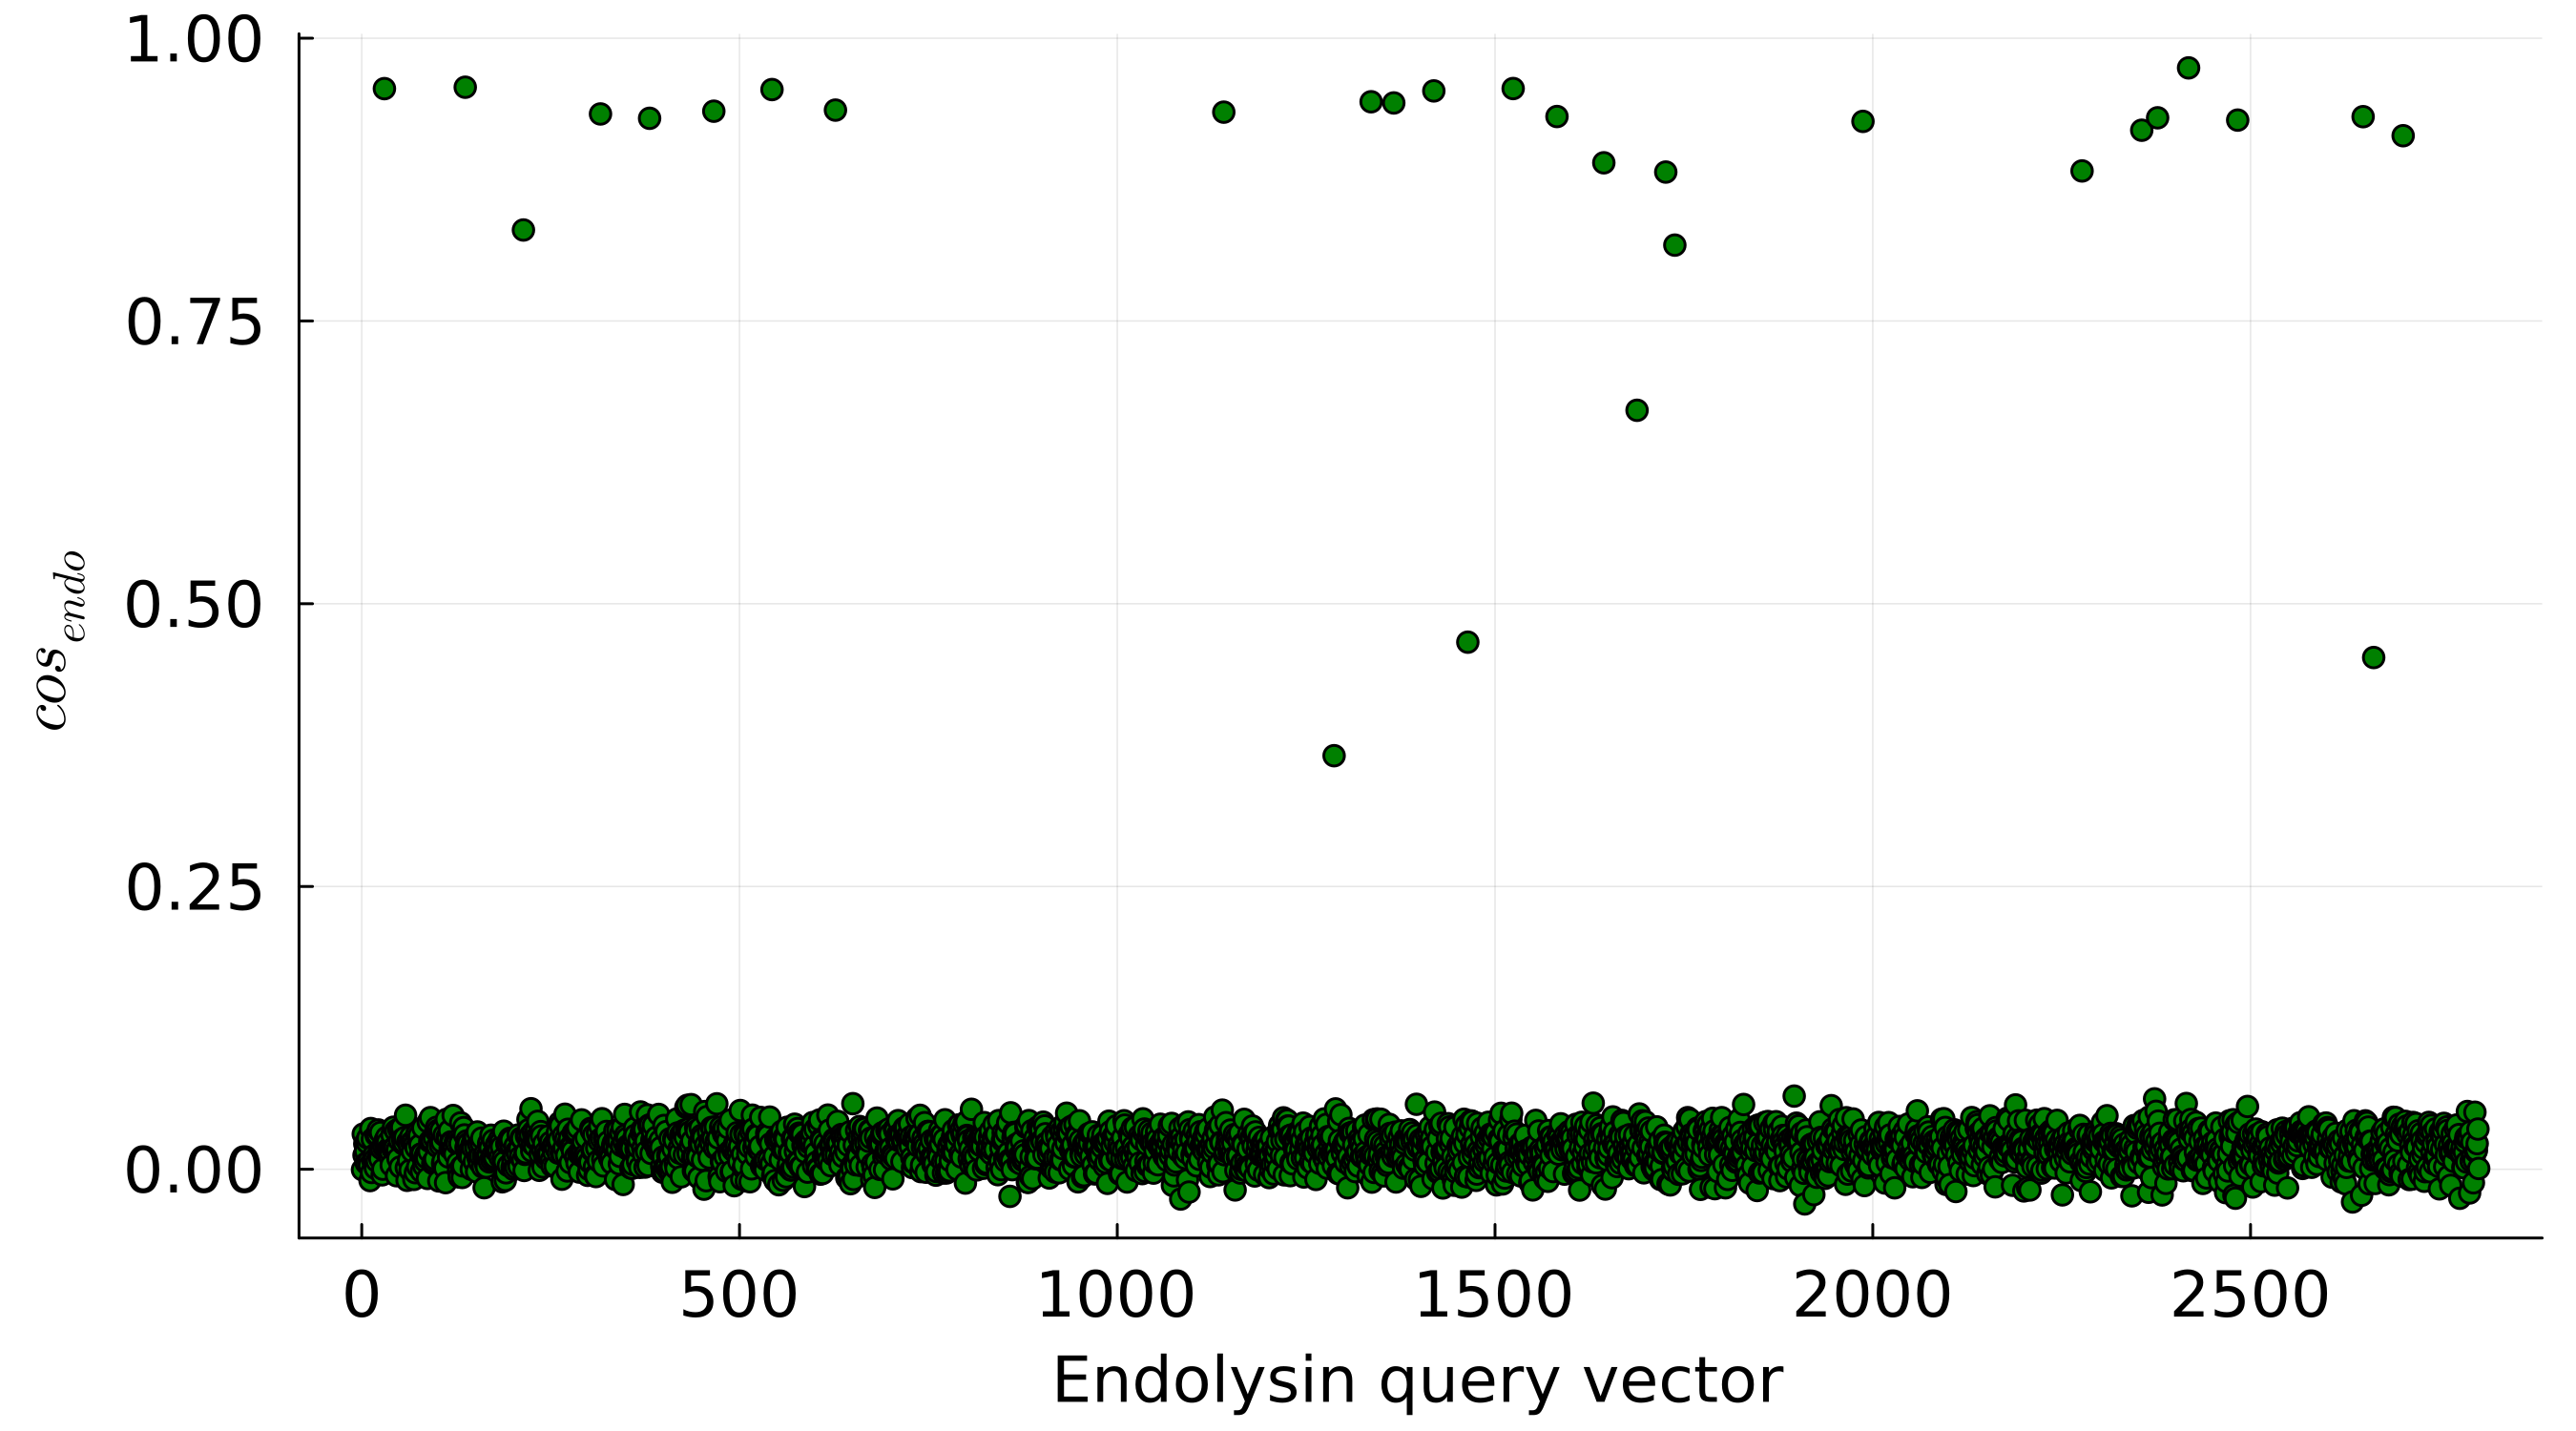
\includegraphics[width=\textwidth]{phalp_cnn_rand_learningE}
        \caption{Endolysins embedded using random amino acid vectors \textit{via} the convolutional embedding method}
        \label{fig:subfig-f}
    \end{subfigure}
    
    \begin{subfigure}{0.48\textwidth}
        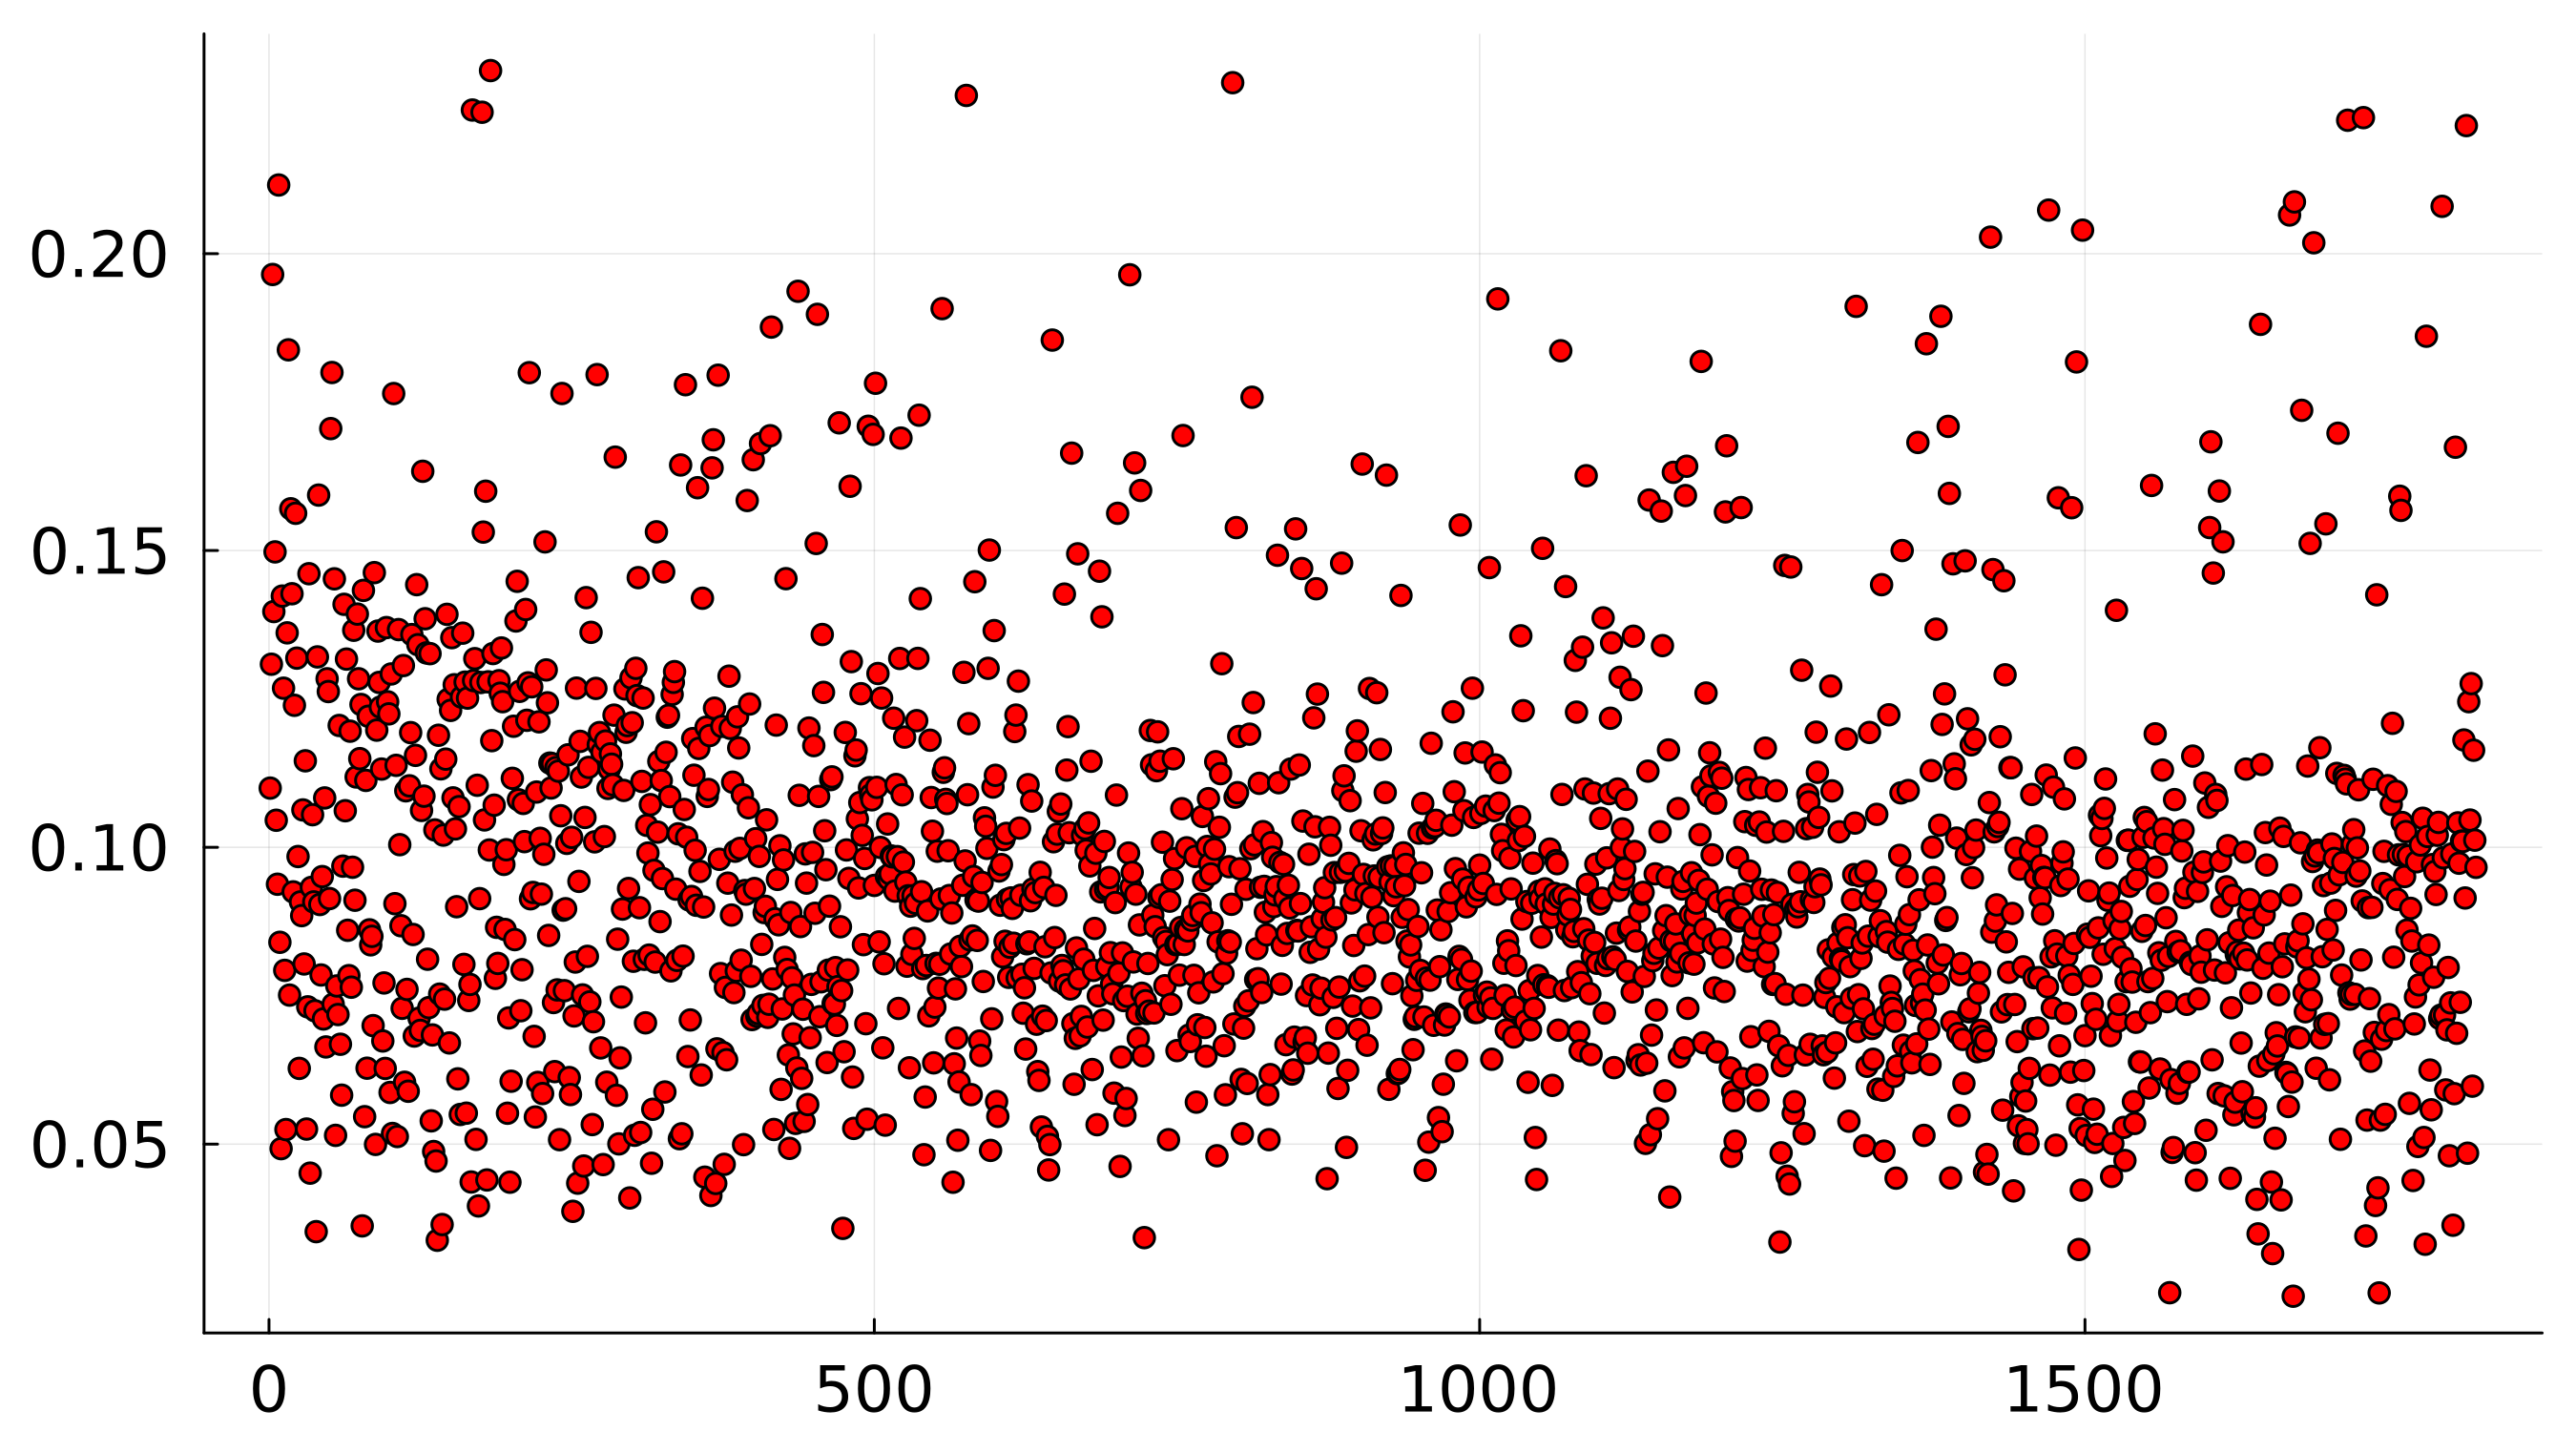
\includegraphics[width=\textwidth]{phalp_cnn_esm_learningV}
        \caption{VALs embedded using projected ESM-2 amino acid vectors \textit{via} the convolutional embedding method}
        \label{fig:subfig-g}
    \end{subfigure}
    \hfill
    \begin{subfigure}{0.48\textwidth}
        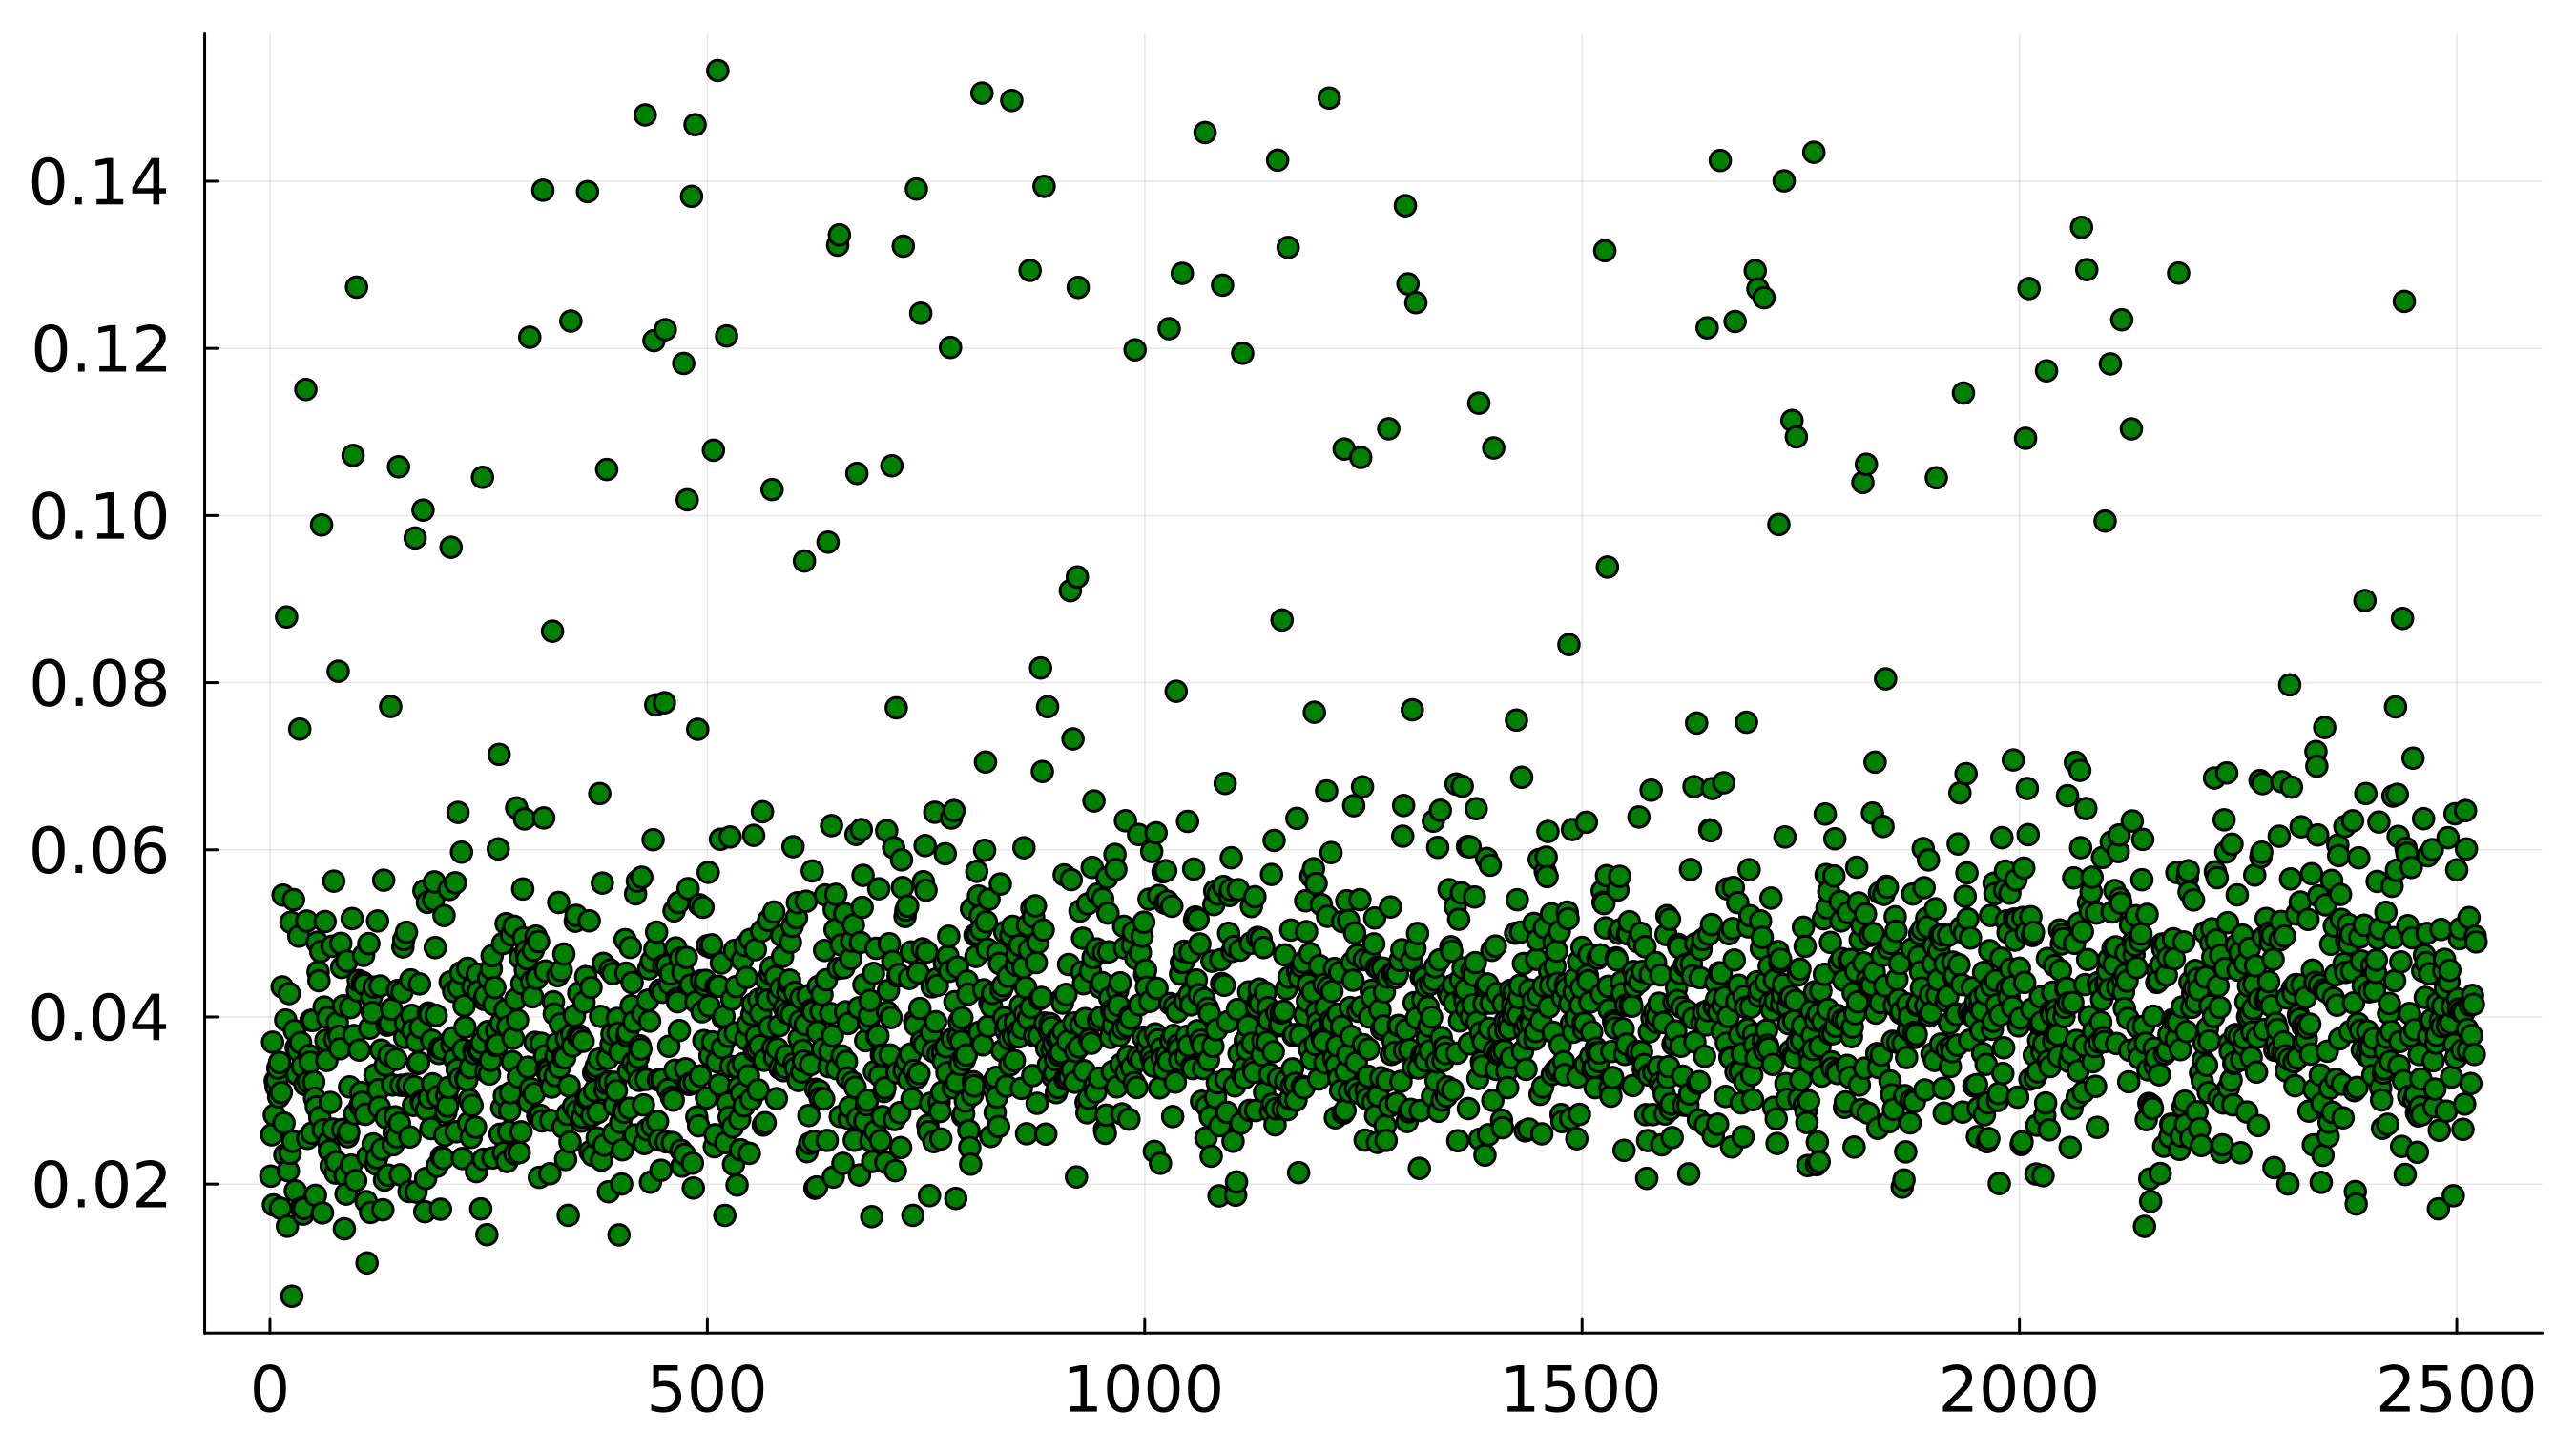
\includegraphics[width=\textwidth]{phalp_cnn_esm_learningE}
        \caption{Endolysins embedded using projected ESM-2 amino acid vectors \textit{via} the convolutional embedding method}
        \label{fig:subfig-h}
    \end{subfigure}
    
    \caption{Cosine similarity between a query vector and the class vector before the weighted update during OnlineHD single-pass training procedure. Trained using hyperdimensional embeddings from all protein sequences in the PhaLP dataset whose types were manually annotated, red representing VALs and green representing endolysins.}
    \label{fig:main}
\end{figure}

Another approach to monitor the training procedure is to track the two class vectors $C_{VAL}$ and $C_{endo}$ individually. For each query vector with a known label $l$, we calculate the cosine similarity $cos(V_{l}, C_{l})$. This method allows us to observe the model's adaptation and refinement of its internal representation of the two classes before it predicts a query vector during the training process. The distance between a query vector and a class vector is proportional to the update weight, so we expect the cosine similarities to generally increase as the model learns. The results are shown in Figure~\ref{fig:main}.

In this case, the VAL vector shows near-consistent weight updates, indicating a high likelihood of the dataset being diverse as the cosine similarities don't seem to decrease. This consistent learning pattern also suggests that the method effectively extracts and learns from the diverse information embedded in the dataset. In general, we see a higher variation in cosine similarities for VAL vectors, which suggests that virion-associated lysins are more diverse in sequence compared to endolysins. This also confirms our earlier findings. We also notice higher overall similarities between the query vectors and the VAL vector when using the BoW-method with projected ESM-2 vectors compared to other embedding methods, which aligns with this model's superior performance. The endolysin vector appears to be updated at a constant rate too, with less variation in similarities. As observed with the VAL vectors, the similarities between the query vectors and the endolysin vector are higher when the embeddings are created using the BoW-method with projected ESM-2 vectors.

\begin{figure}[ht!]
    \centering
    \begin{subfigure}{0.48\textwidth}
        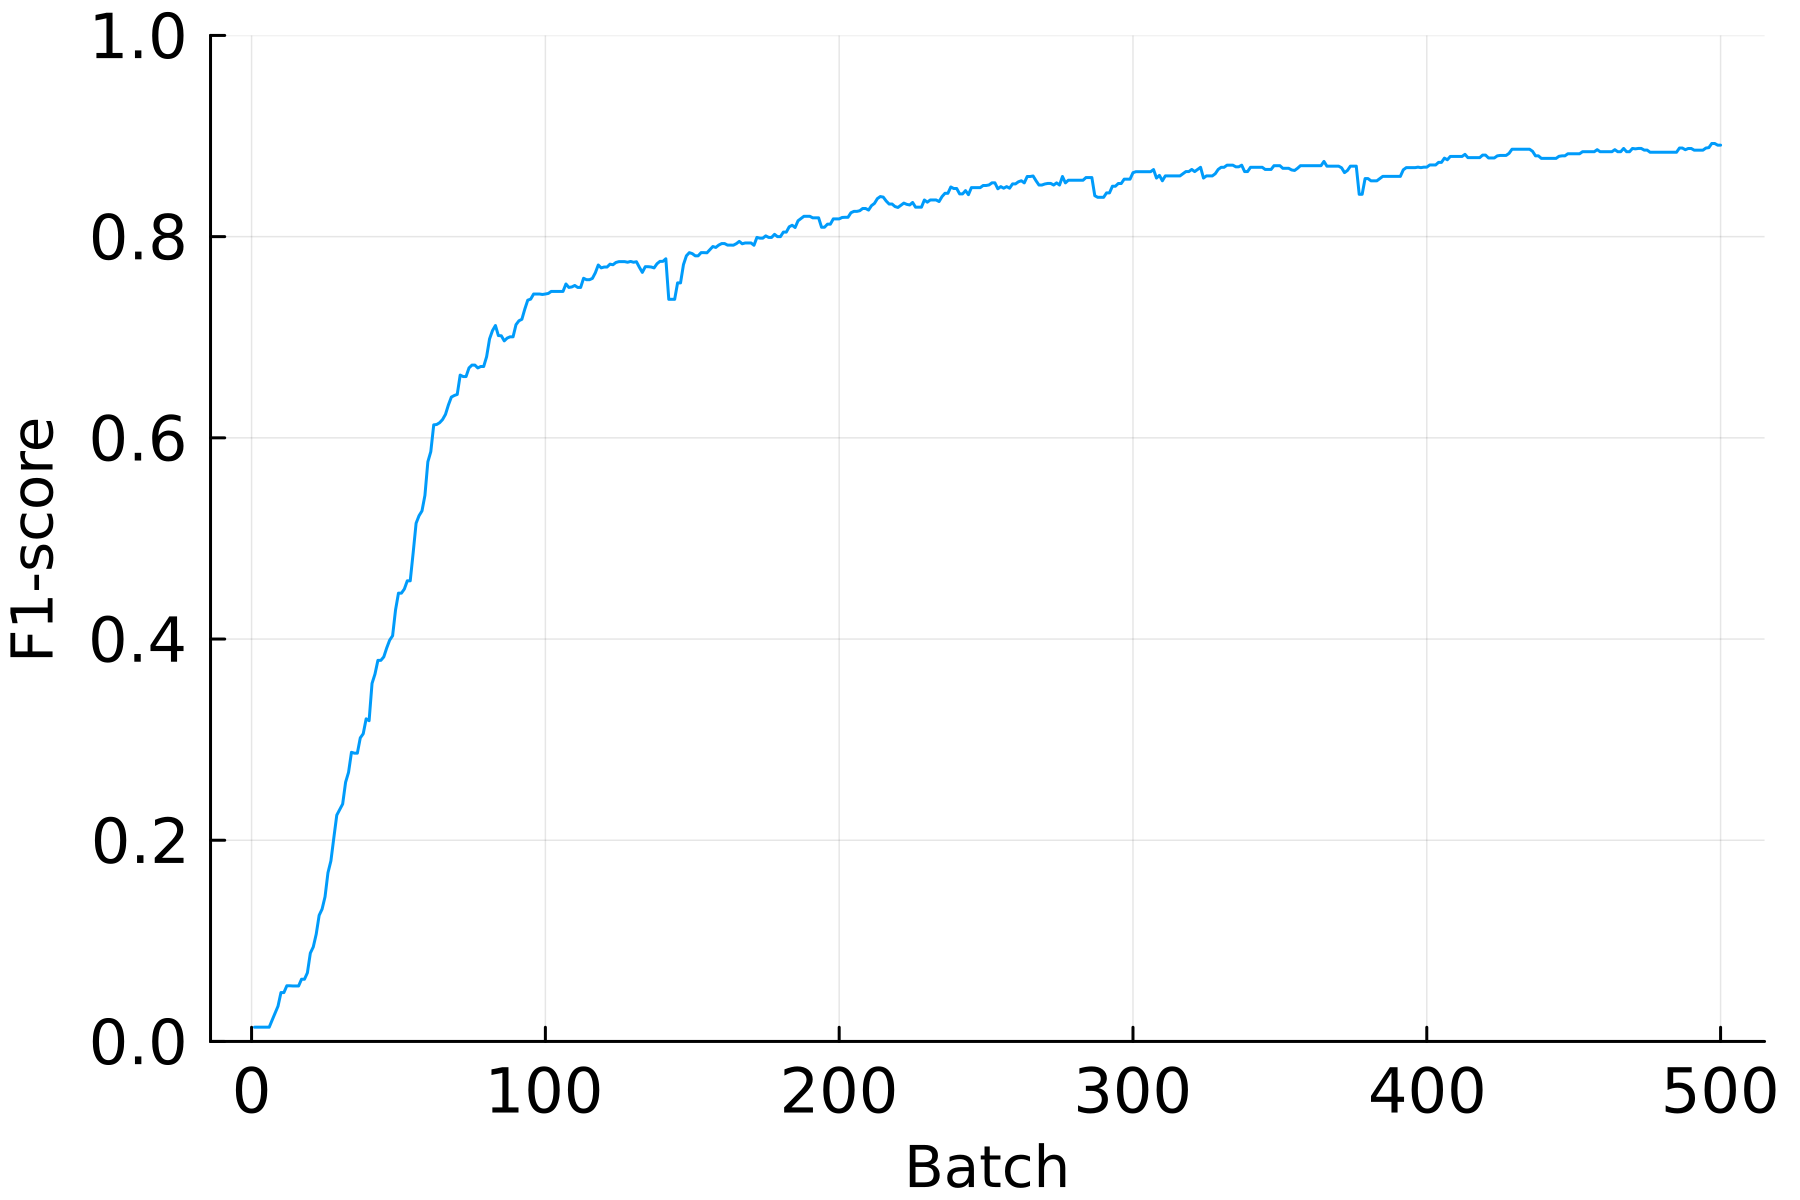
\includegraphics[width=\textwidth]{phalp_bow_rand_score}
        \caption{Embeddings using random amino acid vectors, made \textit{via} the bag-of-words embedding method}
        \label{fig:subfig-a3}
    \end{subfigure}
    \hfill
    \begin{subfigure}{0.48\textwidth}
        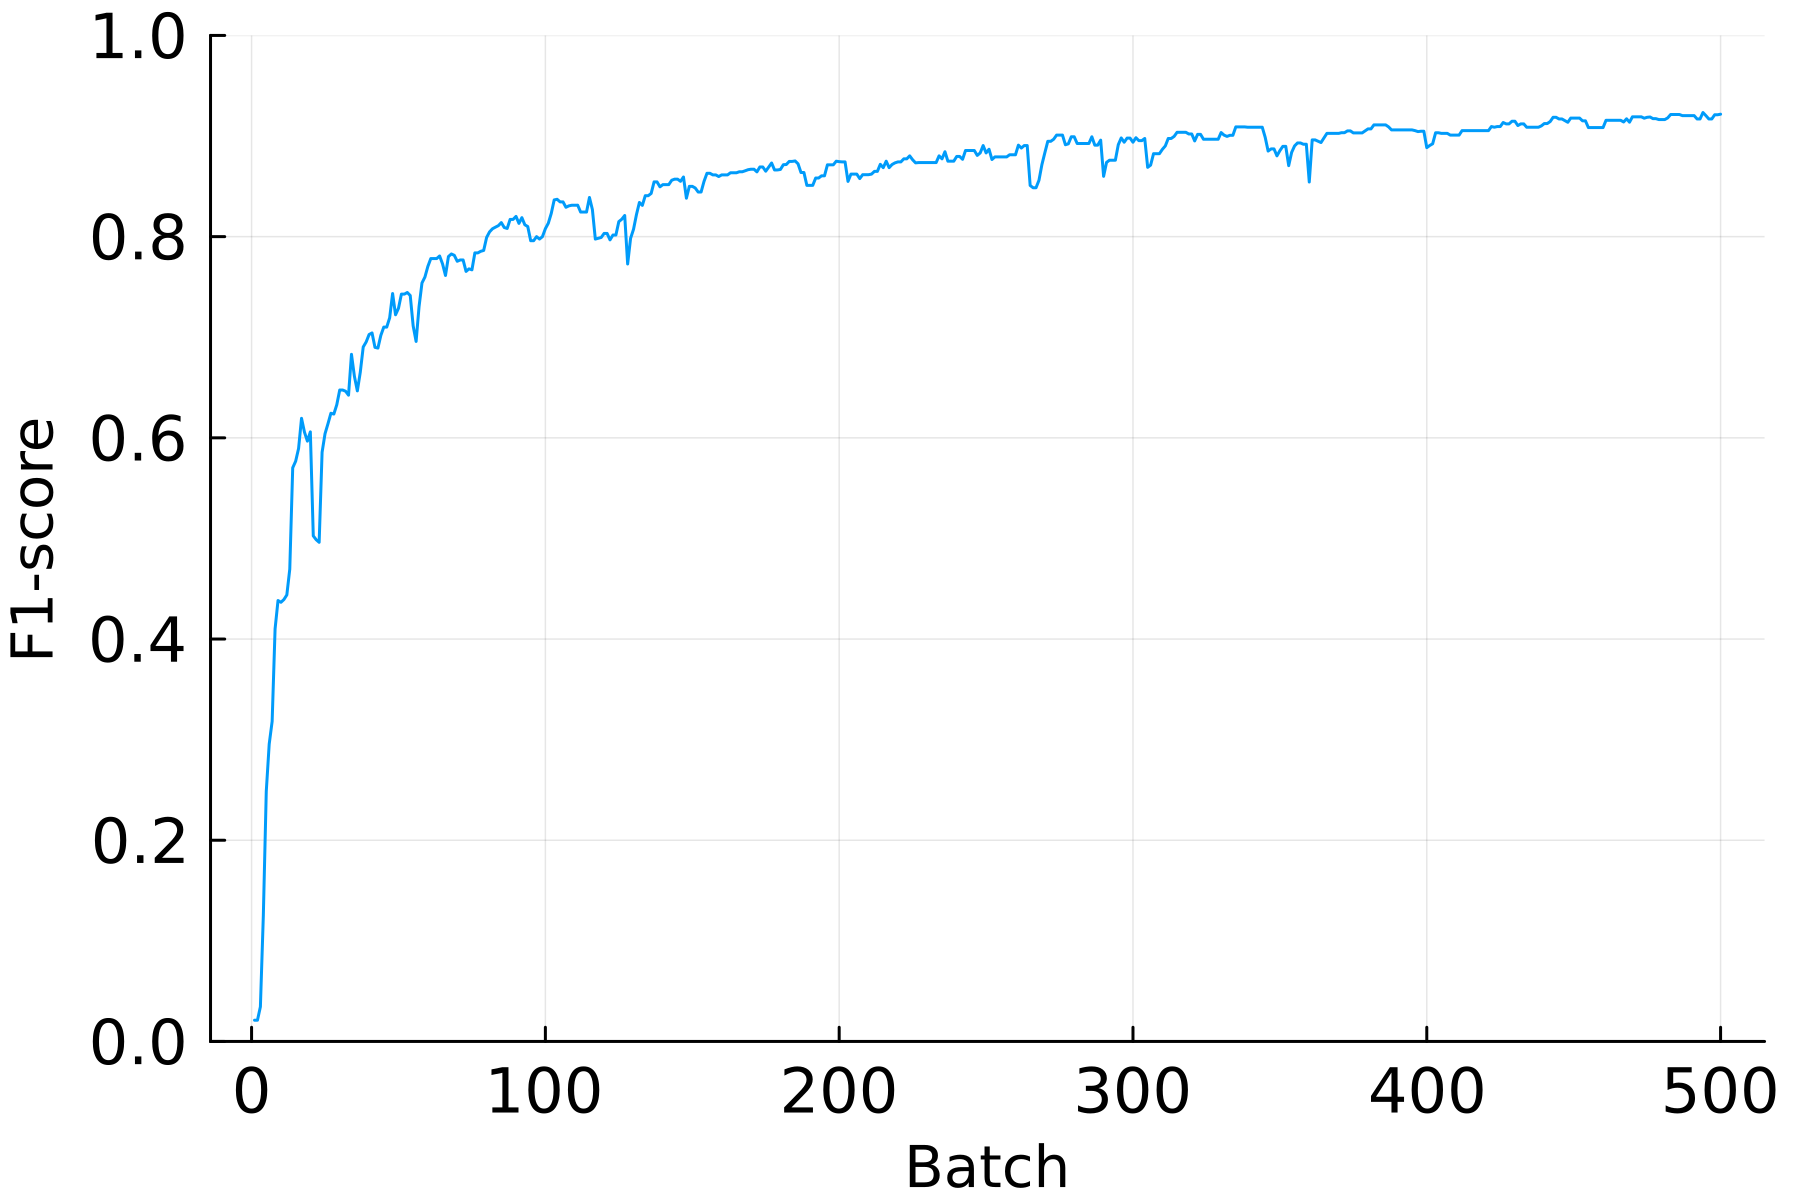
\includegraphics[width=\textwidth]{phalp_bow_esm_score}
        \caption{Embeddings using projected ESM-2 amino acid vectors, made \textit{via} the bag-of-words embedding method}
        \label{fig:subfig-b3}
    \end{subfigure}
    
    \begin{subfigure}{0.48\textwidth}
        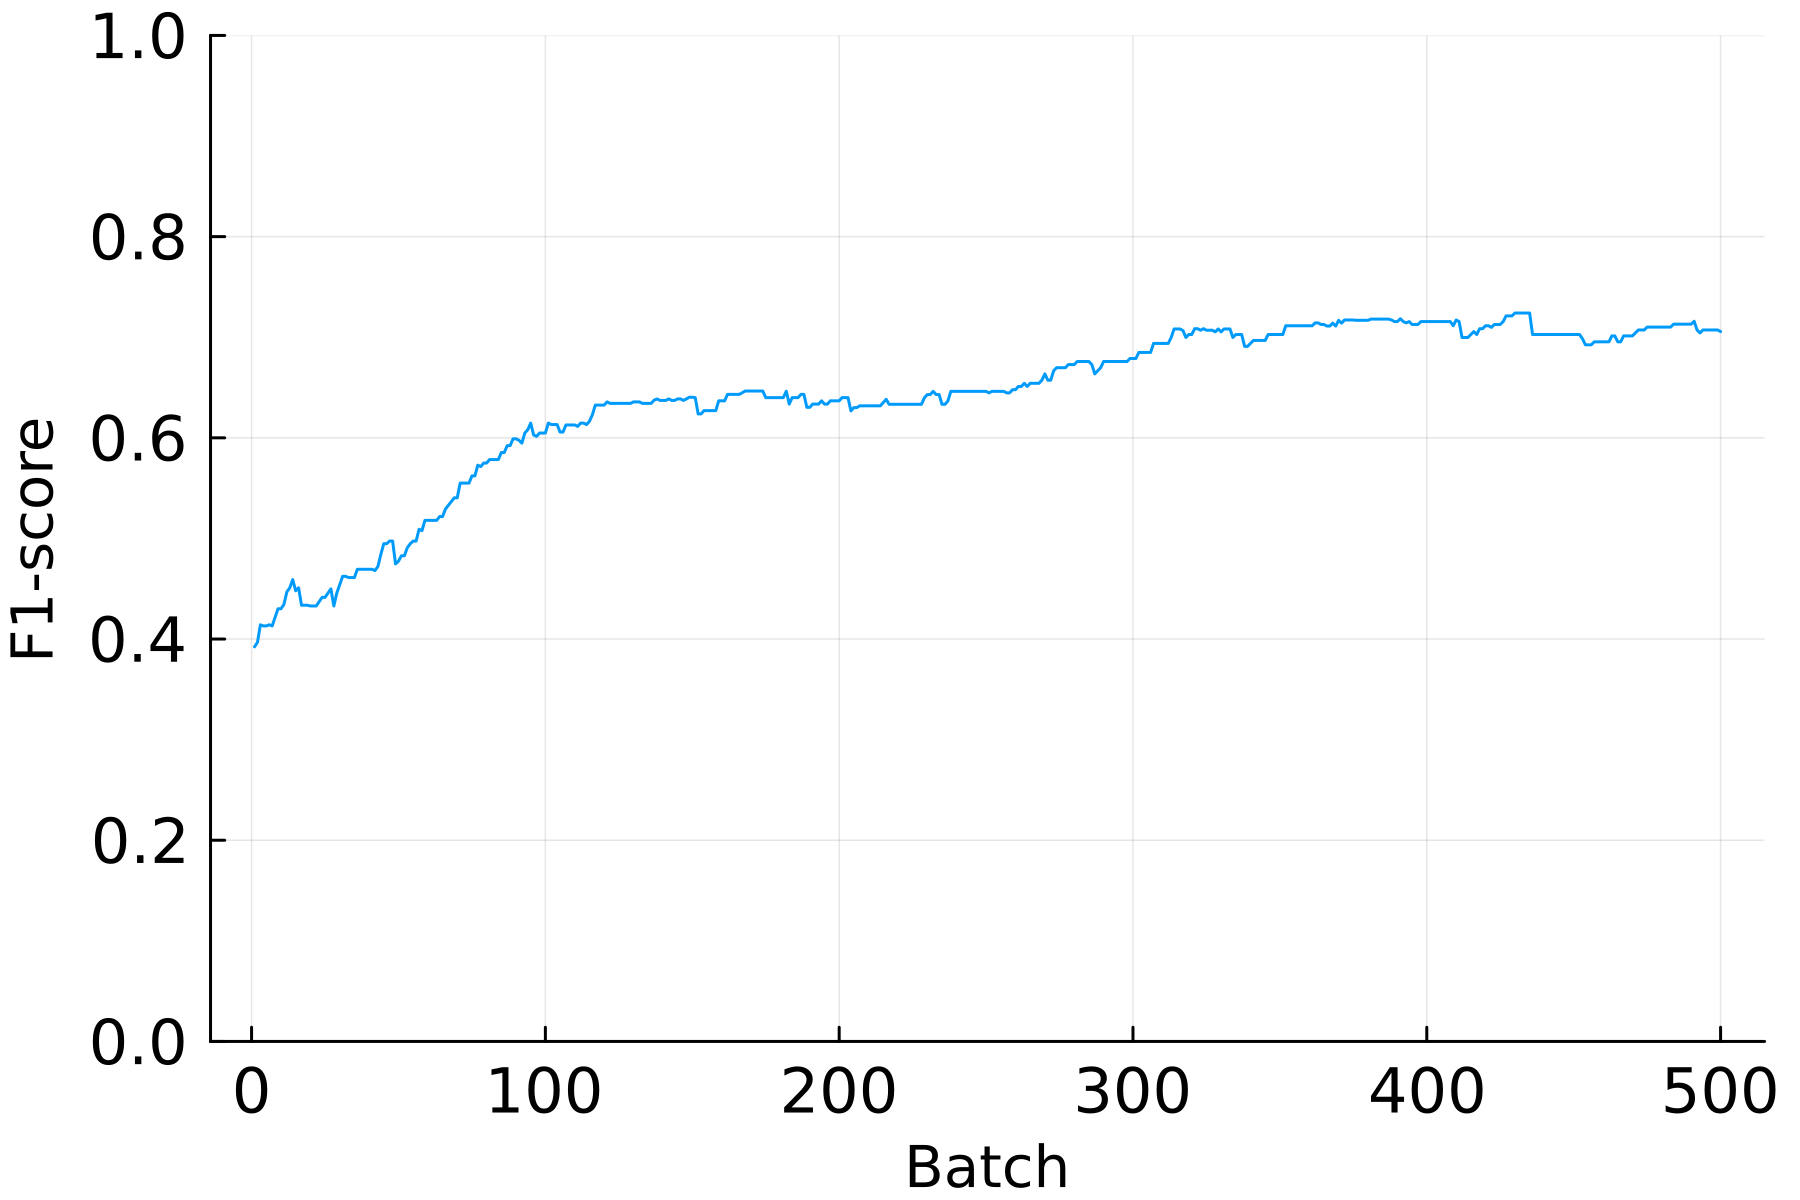
\includegraphics[width=\textwidth]{phalp_cnn_rand_score}
        \caption{Embeddings using random amino acid vectors, made \textit{via} the convolutional embedding method}
        \label{fig:subfig-c3}
    \end{subfigure}
    \hfill
    \begin{subfigure}{0.48\textwidth}
        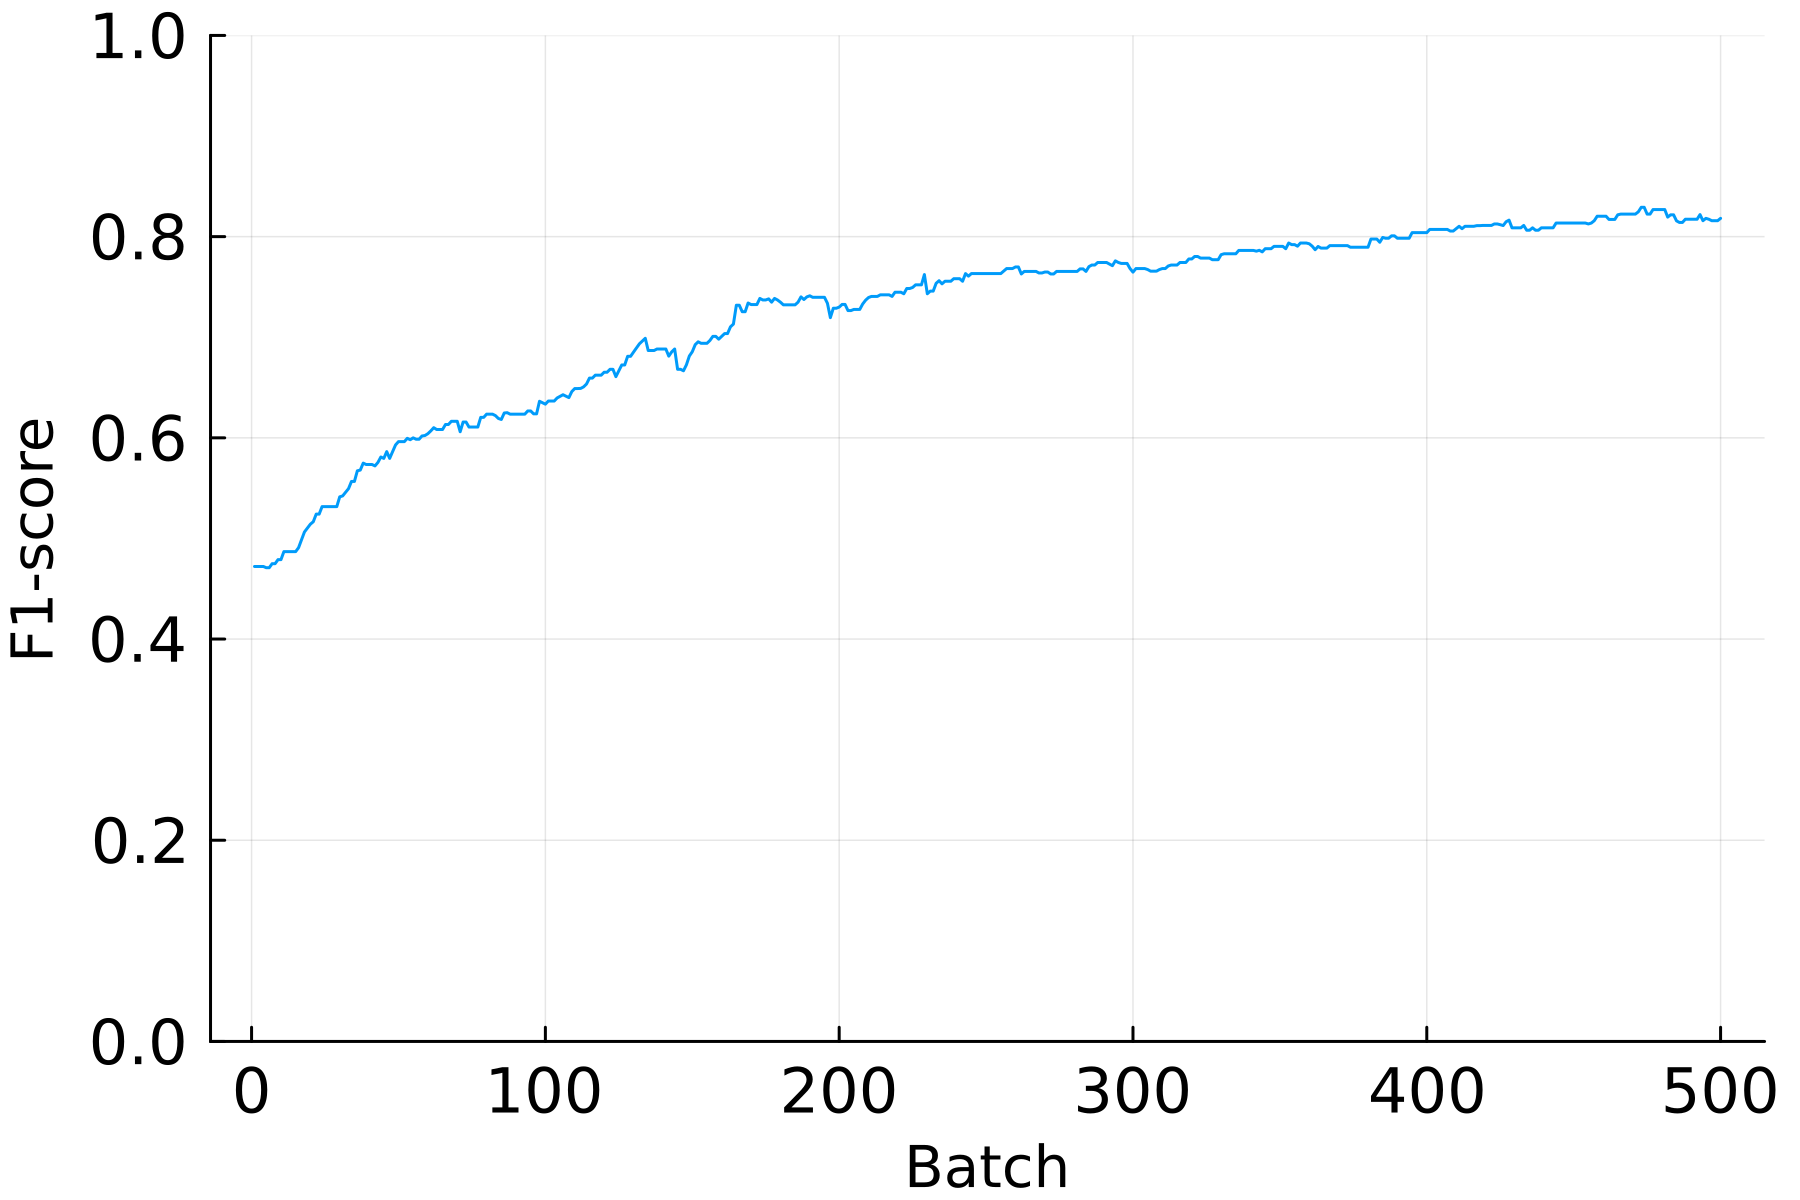
\includegraphics[width=\textwidth]{phalp_cnn_esm_score}
        \caption{Embeddings using projected ESM-2 acid vectors, made \textit{via} the convolutional embedding method}
        \label{fig:subfig-d3}
    \end{subfigure}
    \caption{The F1-score of the OnlineHD single-pass model with a validation set throughout its training procedure. Trained in batches using several kinds of hyperdimensional embeddings from all protein sequences in the PhaLP dataset whose types were manually annotated.}
    \label{fig:main39}
\end{figure}

Instead of looking at the inner workings of the OnlineHD method, the training progress of an OnlineHD model in terms of performance has been monitored. This progress is visualized in Figure~\ref{fig:main39}. Upon initial observation, it is apparent that the models trained with embeddings generated using the convolutional method exhibit superior performance from the outset. This higher starting point might be partially attributed to the random initialization of the model. However, a common characteristic observed across all models is that their performance tends to stagnate after roughly 100 batches, which corresponds to roughly 870 sequences in our case. This observation suggests that hyperdimensional computing-based classification methods may exhibit promising performance and effectively capture essential information, even after being exposed to just a small fraction of the training data, which is an intriguing finding for further exploration.

\section{Discussion}
The low scores of the naive additive methods are likely due to the possibility of oversaturation of the class vectors as discussed in Section~\ref{sec:dis3}. Thus, using the rudimentary model works only for very small datasets, as seen in the examples in chapter~\ref{sec:example}. The ability of this method to learn from a small dataset can be very useful, but backfires in terms of performance when applied to large and diverse datasets as we have seen in the case of classifying protein sequences from the PhaLP database.

This issue is mitigated in the OnlineHD method when used in classifications as it applies weights to class vector updates. This results in a substantial increase in performance. When paired with an iterative retraining procedure its performance comes close to the performance of established machine learning methods paired with binary hyperdimensional sequence embeddings. The OnlineHD methods require real-valued vectors, but still show much higher computational efficiencies compared to established machine learning methods.

From the results in Figures~\ref{fig:main2} and ~\ref{fig:main}, we could not conclude using similarities of query vectors to the class vectors as a metric for training monitoring, as these more likely represent the variety in the training data, especially visible in Figure~\ref{fig:main} as the better-performing models show that they capture more of the intricacies of the input data.

Looking at OnlineHD's performance during its training procedure in Figure~\ref{fig:main39}, we noticed that it is able to capture a lot of information with only a small set of the data, which warrants further study. To further investigate the potential of OnlineHD for protein-level classification in future research, we could investigate how it could classify the sequences based on other types of information present in the PhaLP database such as host type and domains.

Upon comparing various methods for amino acid encoding, we find that dimension-reduction methods tend to capture more information from sequence embeddings created with projected ESM-2 vectors. This observation is consistent with our other finding where we consistently noted an enhanced performance in our classification task using these amino acid vectors. However, our analysis was limited to a single dataset and one specific task; consequently, further investigation is essential. Future studies should focus on the development and evaluation of alternative tasks, while also testing the applicability of this method across various biological datasets.

As for the sequence embedding methods, while no visual differences were discernible after applying PCA to the protein sequences, the results varied subtly depending on the specific model used for classification. Therefore, it appears that there may not be a significant difference in how information is being captured between the two sequence embedding methods in our case. This may indicate that encoding positional information into the k-mers may not be necessary to capture information on protein sequences as the BoW-method captures enough essential information in our case. Nevertheless, future research should discern the potential utility of this in the context of other datasets and predictive tasks.
\chapter[Hyperdimensional computing methods for amino acid-levelp redictions]{Hyperdimensional computing methods\\for amino acid-level\\predictions}
\section{Introduction}
As discussed in section~\ref{ssec:nlp}, state-of-the-art protein language models primarily rely on transformer-based architectures to learn representations of protein sequences and amino acids in the context of other amino acids~\cite{reveiw}. These models have demonstrated their effectiveness in various applications, such as protein function prediction and protein-protein interaction prediction, by capturing complex patterns in amino acid sequences~\cite{esm2}. Moreover, these models are also capable of making detailed predictions at the amino acid level, such as predicting secondary structure. This involves determining local conformations of regions within a protein, such as alpha-helices and beta-sheets, based on the sequence of amino acids. This capability further extends their utility in understanding protein structure and function. However, these models are computationally intensive and may be less suitable for certain tasks or scenarios where computational resources are limited.

In section~\ref{sssec:trans}, we explored the idea of encoding information from a residue's neighborhood into a hyperdimensional vector that represents the residue and its surroundings. This approach allows us to capture local sequence information and can serve as an effective encoding scheme for amino acids. To evaluate the effectiveness of this encoding method, we will employ it as an input for several perceptron-based models.

Perceptron-based models, a type of artificial neural network model, have been employed for various machine learning tasks over the years, including classification and regression problems. The perceptron, one of the simplest and earliest types of neural networks, was proposed by Frank Rosenblatt in 1958~\cite{perceptron}. A perceptron consists of a single artificial neuron that receives multiple input features and computes a weighted sum of these inputs. This weighted sum is then passed through an activation function, which determines the output of the perceptron. The learning process involves adjusting the weights of the input features iteratively, using a rule that minimizes prediction errors on the training data. The perceptron learning algorithm starts with an initial set of weights, typically set to zero or small random values. For each instance in the training data, the perceptron computes the output, compares it with the true label, and updates the weights accordingly. The weight update rule is based on the difference between the predicted output and the true label, multiplied by the learning rate and the input feature value. Single-layer perceptrons consist of an input layer and an output layer of perceptrons, allowing for multiclass classifications. However, they can only solve linearly separable problems, limiting their applicability for more complex tasks.

As single-layer perceptrons can only solve linearly separable problems, researchers developed more complex neural network architectures, such as multi-layer perceptrons (MLP), which consist of multiple layers of artificial neurons connected in a feedforward manner. MLPs can learn non-linear patterns in the data by using non-linear activation functions (e.g., sigmoid, tanh, ReLU) and employing backpropagation for weight updates~\cite{mlp}. This enhanced ability to model non-linear relationships allows MLPs to tackle a wider range of problems.

By combining the residue neighborhood encoding method with perceptron-based models, we could develop more computationally efficient alternatives to state-of-the-art transformer-based models. These models may provide valuable insights into protein sequences and amino acids while being more suitable for scenarios with limited computational resources. 

The aim of this chapter is to design and implement a simple perceptron-based neural network that utilizes hyperdimensional vectors of residues in a protein sequence as inputs. The goal is to train the network to discern and learn the secondary structure of these residues based on their surrounding counterparts. Ultimately, this should enable our model to accurately and efficiently predict the secondary structures of residues in protein sequences whose structure is unknown.

\section{Methods}
We built straightforward perceptron-based neural networks that take as input a hyperdimensional vector, in particular a neighborhood-encoded amino acid vector made as described in section~\ref{sssec:trans}. It should then output the amino acid's secondary structure, either 3- or 8-state as shown in Figure~\ref{fig:pipe2}.

\begin{figure}[H]
    \centering
    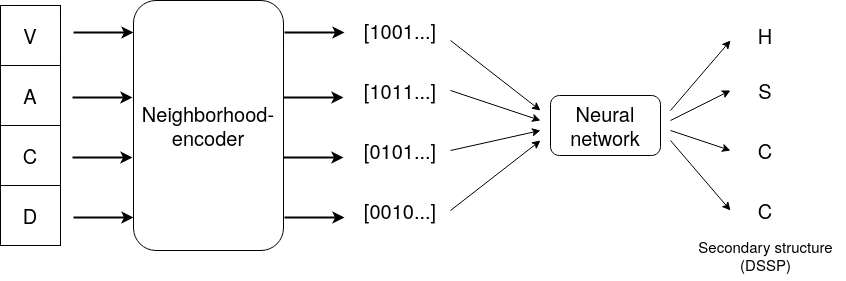
\includegraphics[scale = 0.43]{pipeline2}
    \caption{A simple demonstration of our pipeline to classify amino acids on their secondary structure based on their neighborhood-encoded vectors. First, a residue is encoded by neighborhood-encoding as discussed in section~\ref{sssec:trans}. Then, this vector is used as an input for a trained neural network to predict its secondary structure state. This is done for every residue in every given protein sequence.}\label{fig:pipe2}
\end{figure}

We used the training dataset compiled by Klausen \textit{et al.} for their model protein language model NetsurfP 2.0~\cite{netsurf} as our training dataset. It contains 10,337 protein sequences obtained from the Protein Data Bank (PDB)~\cite{pdb}. Each residue in these sequences is annotated with its 3- and 8-class secondary structure classification according to \textit{Define Secondary Structure of Proteins} (DSSP)~\cite{dssp}, providing a comprehensive description of the protein's structural properties. All residues have been encoded using our neighborhood-encoder as described in section~\ref{sssec:trans} with $n=25$ and $n=100$ using random hyperdimensional vectors for each amino acid. Due to computational memory constraints, we randomly selected 60 \% of the sequences from the original dataset for training and validation (80 \% and 20 \% respectively), ensuring a representative sample of the data.

In summary, we have four distinct supervised training sets. The first model is trained on neighborhood-encodings of range $n=25$ with 3-state secondary structure labels. The second model also uses neighborhood-encodings of range $n=25$, but with 8-state secondary structure labels. The third model is trained on neighborhood-encodings of range $n=100$, using 3-state secondary structure labels. Finally, the fourth model uses neighborhood-encodings of range $n=100$ and 8-state secondary structure labels.

As for the perceptron-based methods, to decrease the computational time, we opted to build, train and evaluate the model in Python due to its support for computations on GPUs on our systems. We employed PyTorch Lightning v1.8.4 for model construction and training on a high-performance computing (HPC) cluster equipped with an NVIDIA V100 GPU. The model comprised fully-connected layers with an input layer size equal to the dimension of the hyperdimensional vectors (10,000 in this case). Depending on the secondary structure classification desired, the output layer size was set to either 3 or 8 depending on the secondary structure classification. We used a batch size of 128 during training. Between each layer, we incorporated a ReLU (Rectified Linear Unit) activation function to introduce non-linearity into the model. The training loss was monitored using cross-entropy loss. To optimize the model, we employed the widely-used ADAM optimizer. We evaluated various configurations and hyperparameters to determine the best-performing but still computationally feasible approach as shown in Table~\ref{tab:casp8}

\begin{table}[h]
    \caption{Overview of model configurations and hyperparameters tested}
    \label{tab:casp8}
    \centering
    \begin{tabular}{l|ccc}
        \toprule
         & Epochs & Learning rate & Size hidden layer(s)\\
        \midrule
        \textbf{SLP} & 100 & 0.03 & /\\
        \hline
        \textbf{1-layer MLP} & 50 & 0.003 & 500\\
        \hline
        \textbf{10-layer MLP} & 200 & 0.0003 & \makecell{8000-5000-2000-1000-800-\\500-200-100-50-20}\\
        \bottomrule
    \end{tabular}
  \end{table}

As test datasets, we opted to use CB513~\cite{cb513} and CASP12~\cite{casp12} (compiled by the developers of NetSurfP 2.0~\cite{netsurf}) since they are easily attainable and commonly used by researchers as benchmark datasets for protein language models. The MLP model with 10 hidden layers was trained and then evaluated using these test datasets. For extra validation, random data was generated in the form of random hyperdimensional vectors with randomly given labels.

\section{Results}
Figure~\ref{fig:she} presents the outcome of the training procedure of all perceptron-based configurations with $n=25$ and dssp3-classification. They show notable issues with the SLP models' ability to train effectively on our dataset. This is signaled by the substantial fluctuations in both loss and validation performance, a trend suggesting an inherent instability in the learning process of this model. The SLP model also displayed a abnoramlly high error compared to the other configurations. The 1-layer MLP model also exhibits problematic behavior, as it does not seem to learn as seen in its constant loss-curve. On top of that, it predicts only one single class during validation (the class with the highest proportion), resulting in a large discrepancy between the accuracy and F1-score. All of this could be attributed to the simplicity of these models, which might not have the capacity to capture the complex patterns in the data. These limitations lead to our decision to discontinue further investigations and experimentation with these particular models. These behaviors were seen throughout all types of datasets (both $n$s and dssp-classifications) as seen in Figures~\ref{fig:she2},~\ref{fig:she3} and~\ref{fig:she4} in the appendices.  

In contrast to the SLP and the 1-layer MLP models, the performance of the much deeper 10-layer MLP model demonstrates much more stable and consistent behavior throughout the training process, as evidenced by the performance and loss metrics, even though the resulting performance remains generally low. Although this stability may partially result from the lower learning rate, the model's computational feasibility made it an option for further investigation, prompting us to select this 133,343,733-parameter model for our subsequent tests with various datasets and comparisons with other state-of-the-art methods.

\begin{table}[h]
    \caption{Accuracies of secondary structure classification of a 10-layer MLP model trained on 60 \% of NetSurfP 2.0's training data encoded into different kinds of hyperdimensional embeddings made with neighborhood-encoding ($n = 25$ and $n=100$). Tested on the CASP12 and CB513 dataset. Performance with randomly generated data was also assessed.}
    \label{tab:casp}
    \centering
    \begin{tabular}{l|cc|cc|cc}
        \toprule
        \textbf{Accuracy} & \multicolumn{2}{c|}{CASP12} & \multicolumn{2}{c|}{CB513} & \multicolumn{2}{c|}{Random}\\
        & ss3 & ss8 & ss3 & ss8 & ss3 & ss8\\
        \midrule
        \textbf{n25} & 36.9 & 24.88 & 35.48 & 21.01 & 34.11 & 21.09 \\
        \textbf{n100} & 39.33 & 23.13 & 37.61 & 20.86 & 38.74 & 20.53\\
        \bottomrule
    \end{tabular}
\end{table}

\begin{table}[h]
    \caption{F1-scores of secondary structure classification of a 10-layer MLP model trained on 60 \% of NetSurfP 2.0's training data encoded into different kinds of hyperdimensional embeddings made with neighborhood-encoding ($n = 25$ and $n=100$). Tested on the CASP12 and CB513 dataset. Performance with randomly generated data was also assessed.}
    \label{tab:casp2}
    \centering
    \begin{tabular}{l|cc|cc|cc}
        \toprule
        \textbf{F1} & \multicolumn{2}{c|}{CASP12} & \multicolumn{2}{c|}{CB513} & \multicolumn{2}{c}{Random}\\
        & ss3 & ss8 & ss3 & ss8 & ss3 & ss8 \\
        \midrule
        \textbf{n25} & 37.50 & 18.61 & 35.52 & 15.30 & 34.35 & 14.79\\
        \textbf{n100} & 37.19 & 20.25 & 35.68 & 18.03 & 36.07 & 17.80\\
        \bottomrule
    \end{tabular}
\end{table}

\begin{table}[h]
    \caption{Accuracies of secondary structure classification of state-of-the-art protein language models. Tested on 3 and 8 secondary structure classifications of the CASP12 and CB513 dataset.}
    \label{tab:casp3}
    \centering
    \begin{tabular}{lcc|cc}
        \toprule
        \textbf{Accuracy} & \multicolumn{2}{c|}{CASP12} & \multicolumn{2}{c|}{CB513}\\
        & ss3 & ss8 & ss3 & ss8\\
        \midrule
        \textbf{ESM-1b} & 76.9 & 83.9 & 66.0 & 70.2\\
        \textbf{NetSurfP 2.0} & 82.0 & 84.5 & 66.9 & 71.3\\
        \textbf{NetSurfP 3.0} & 79.1 & 84.5 & 66.9 & 71.1\\
        \textbf{ProtT5-XL-U50} & 77.5 & 86.2 & 70.5 & 74.5\\
        \bottomrule
    \end{tabular}
  \end{table}

The fully trained 10-layer MLP models were evaluated on the test datasets with the results summarized in Table~\ref{tab:casp} and Table~\ref{tab:casp2}. To validate our findings, we also generated a randomly generated dataset for comparison. Disappointingly, the model's performance on the test data only slightly surpassed its own performance on the randomly generated data, meaning that our model is not able to accurately predict the secondary structure of an amino acid based on its neighborhood-encoding as compared to state-of-the-art protein language models shown in Table~\ref{tab:casp3}.

\begin{figure}[H]
    \centering
    \begin{minipage}[b]{.6\textwidth}
        \begin{subfigure}[b]{\textwidth}
        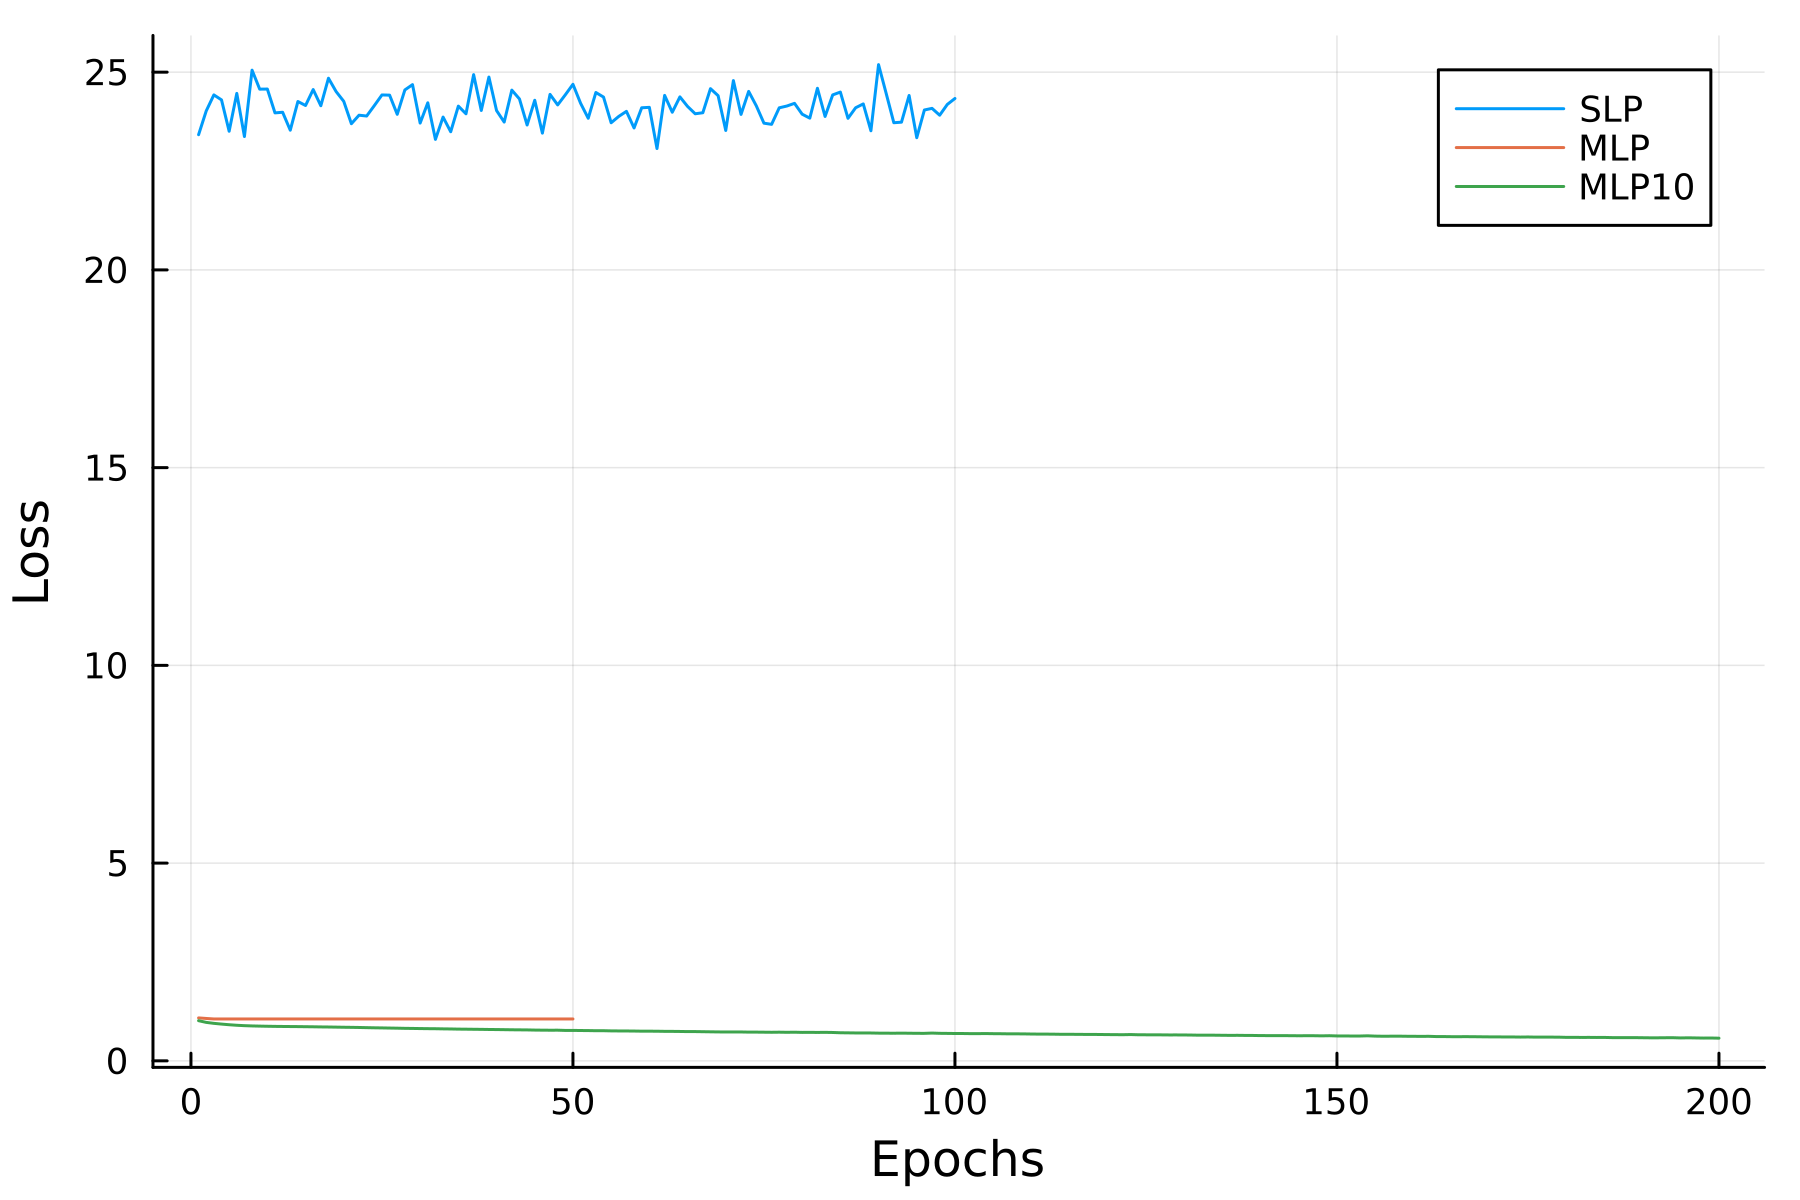
\includegraphics[width=\textwidth]{loss_plot_25_3}
        \caption{Training losses}
        \label{fig:loss}
    \end{subfigure}
    \end{minipage}
    \\
    \centering
    \begin{minipage}[b]{.6\textwidth}
    \begin{subfigure}[b]{\textwidth}
        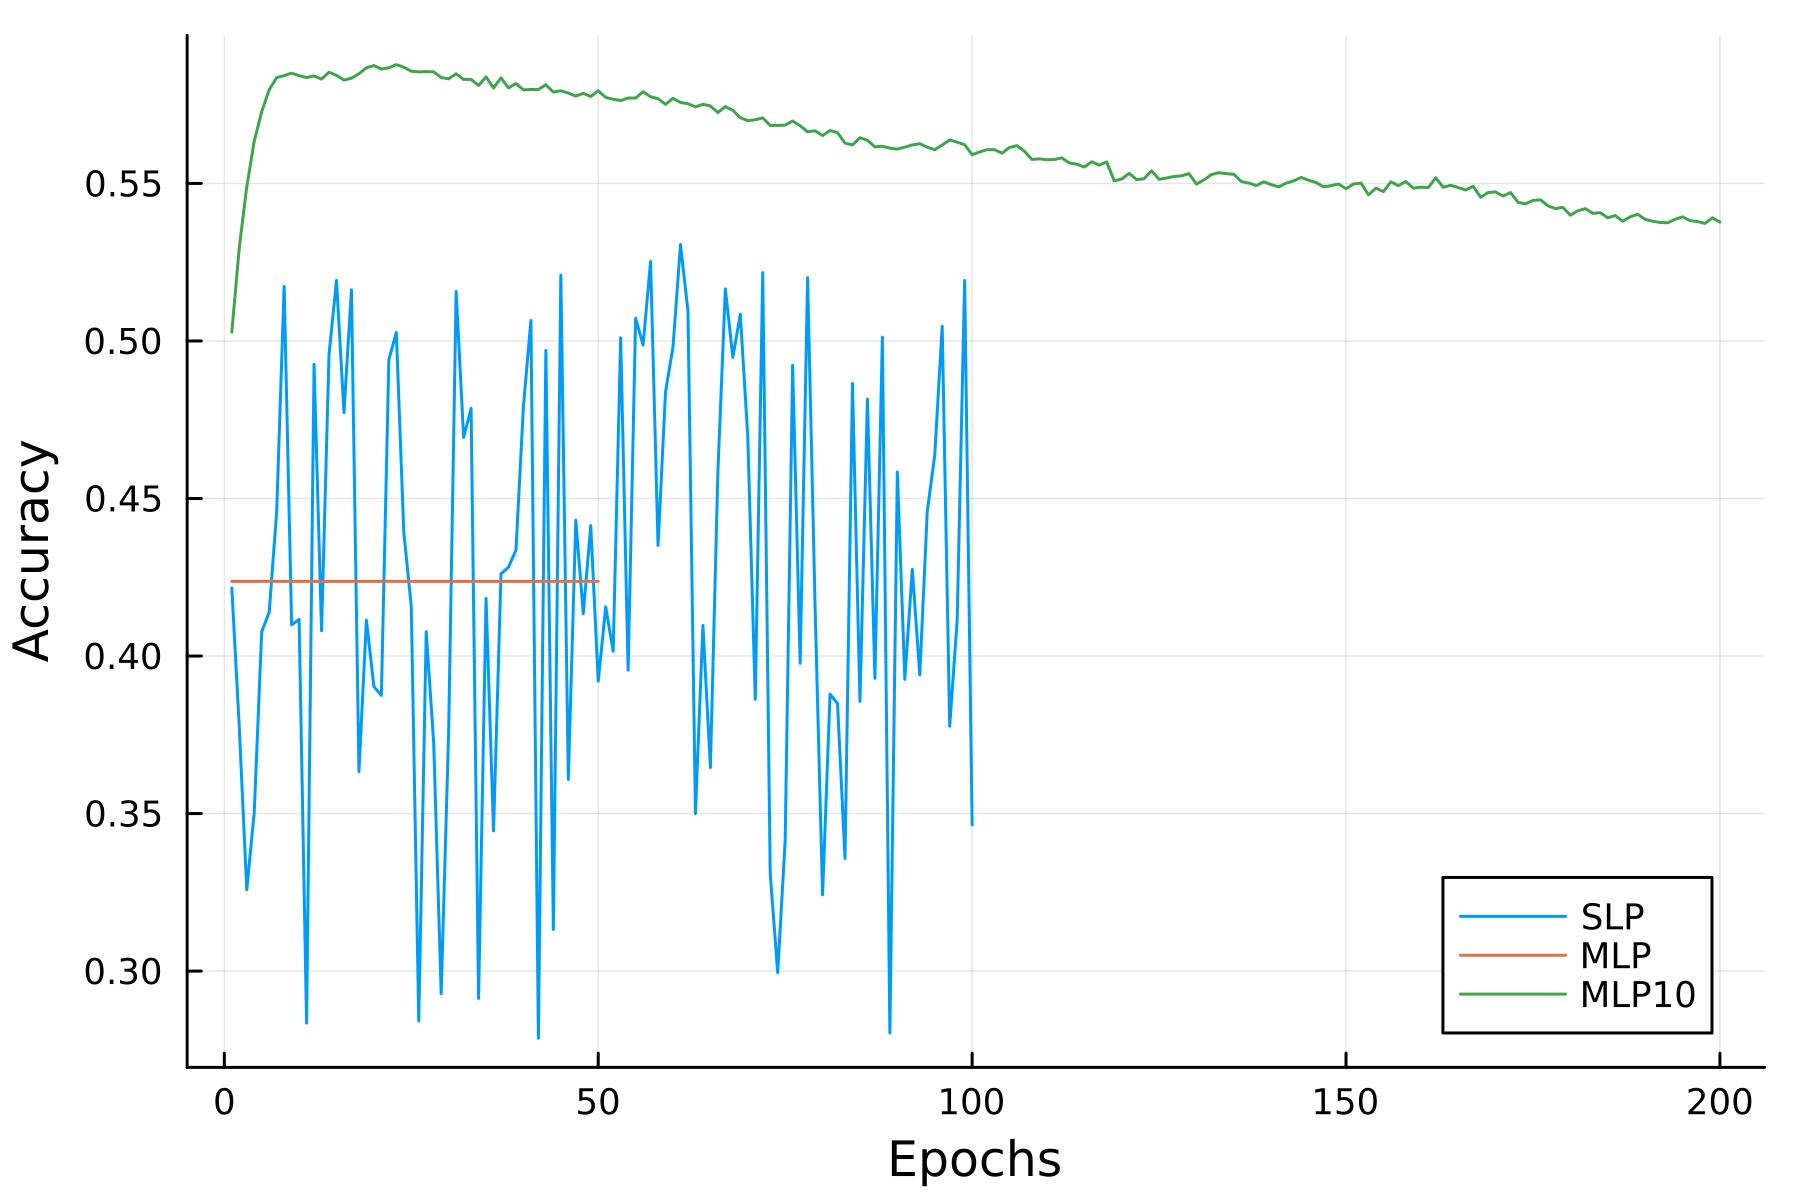
\includegraphics[width=\textwidth]{accuracy_plot_25_3}
        \caption{Accuracies}
        \label{fig:accuracy}
    \end{subfigure}
    \end{minipage}
    \\
    \centering
    \begin{minipage}[b]{.6\textwidth}
    \begin{subfigure}[b]{\textwidth}
        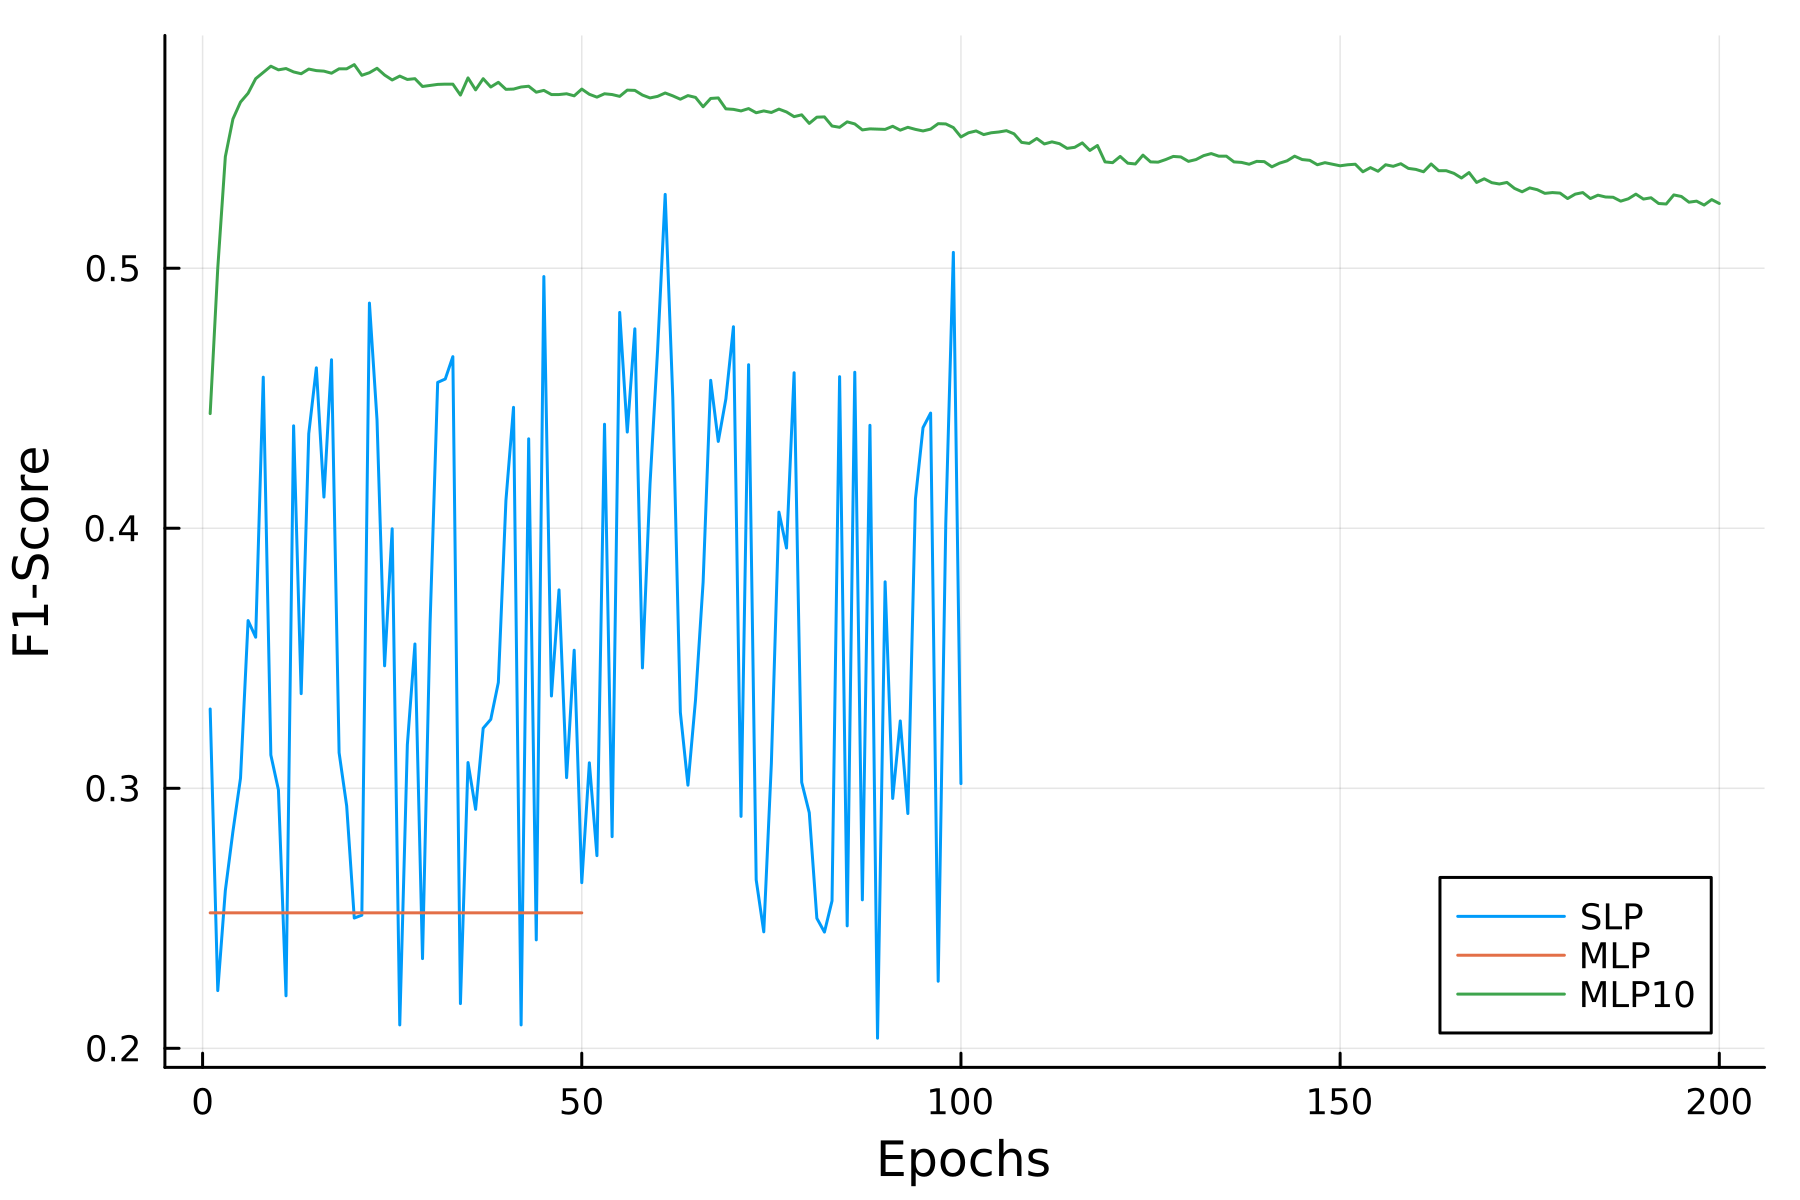
\includegraphics[width=\textwidth]{f1_plot_25_3}
        \caption{F1-scores}\label{fig:f1}
    \end{subfigure}
    \end{minipage}
    \caption{(a) cross-entropy losses (b) accuracies (c) F1-scores of all perceptron-based configurations tested. Trained with neighborhood-encodings of 60 \% of the training dataset of NetSurfP 2.0. Here $n=25$ and the secondary structure classification is dssp3-based. Note that the SLP and 1-layer MLP model was evaluated using fewer epochs than their 10-layer counterpart.}\label{fig:she}
    \end{figure}

\section{Discussion}
Our exploration into the use of various perceptron-based neural network models for protein secondary structure prediction has yielded several insights. The overarching observation from our results is that our models have not effectively learned from the data. This suggests a couple of potential areas for improvement.

Firstly, the relative simplicity of our neural network models may be a limiting factor. The high-dimensional sparse vectors that represent our data may require a more complex model to capture the intricate patterns within the data effectively. This could involve exploring more sophisticated architectures, such as deeper networks or alternative architectures. A hyperdimensional computing-based method such as OnlineHD might be an interesting learning method too for later research.

Secondly, the neighborhood-encoding algorithm we employed may require further refinement. The quality of the embeddings produced by this algorithm directly impacts the ability of the model to learn. Optimizing this algorithm to produce more informative or discriminative embeddings could potentially enhance the learning capability of our models. As said earlier, there might be a case of oversaturation in the vectors and therefore a loss of information on the complex intricacies in the data since binary vectors were used to encode the data. Interesting avenues might include using real-valued vectors to generate neighborhood-encodings. This algorithm could then be coupled with weighted additions to avoid oversaturation of vectors. Instead of relying solely on random amino acid vectors for neighborhood-encoding the residues, future research could investigate the potential utility of alternative amino acid representations, such as the projected ESM-2 embeddings, either real-valued or binary.

Lastly, the size of the training dataset could also be a contributing factor. Given the computational constraints of this study, we were limited in the amount of data we could use for training. However, machine learning models, especially deep neural networks, often benefit from larger datasets. Increasing the size of the training dataset could provide our models with more examples to learn from, potentially improving their performance.

In order to benchmark our study against the capabilities of state-of-the-art protein language models, we collected the available results of other protein language models on similar experiments. The models include ESM-1b~\cite{esm}, NetSurfP 2.0~\cite{netsurf}, its successor NetSurfP 3.0~\cite{netsurf3} and ProtTrans' best-performing model; ProtT5-XL-U50~\cite{prottrans}. ESM-1b is a model by Meta AI, trained on a large corpus of approximately 86 billion amino acid residues. It consists of around 670 million parameters and utilizes a transformer architecture together with evolutionary data. NetsurfP 2.0 and its successor NetSurf 3.0 are models comprising convolutional neural network (CNN) and bidirectional long short-term (biLSTM) layers. Despite not relying on a transformer-based architecture and having been trained on a comparatively smaller dataset, they exhibit state-of-the-art performance. The distinction between these two methods lies in their input configurations. ProtT5-XL-U50 is a large transformer-based model comprising 3 billion parameters, trained on UniRef50 which comprises roughly 45 million sequences~\cite{uniref}.

When compared to the performance of state-of-the-art protein language models in Table~\ref{tab:casp3}, our models fall short in performance. This underscores the complexity of protein secondary structure prediction and the need for models that can effectively learn from the intricate patterns in the data.


% ------------ REFERENCES ------------
% Here you have your bibliography created
\addcontentsline{toc}{chapter}{Bibliography} %show bibliography in TOC
\bibliographystyle{unsrt}  %apalike,phdbib.bst
\bibliography{Thesis_bib}
% Here you insert your appendices
\appendix
\begin{appendices}

% Dit voegt het woord Bijlage toe aan de titel!
\titleformat{\chapter} % command
  [display] % shape
  {\fontsize{18}{22} \selectfont \coltitle } % format
  {\MakeUppercase{\chaptertitlename \ \thechapter}} % the label
  {-2ex} %separator space
  {\fontsize{24}{32} \selectfont \bf \raggedright \MakeUppercase{\uline{#1}}} %before code
  { } %aft%after code


\chapter{Additional information on Chapter 3}\label{app:chp3}
\begin{figure}[h!]
    \centering
    \begin{subfigure}{0.48\textwidth}
        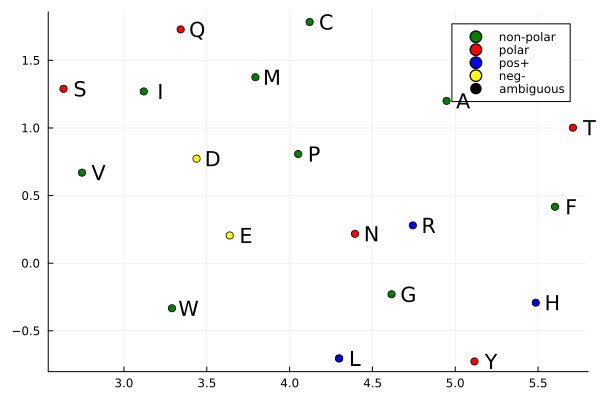
\includegraphics[width=\textwidth]{ur4tr_emb}
        \caption{Made starting from random hyperdimensional vectors for each amino acid, $k=4$.}
        \label{fig:AAtr4ru}
    \end{subfigure}
    \hfill
    \begin{subfigure}{0.48\textwidth}
        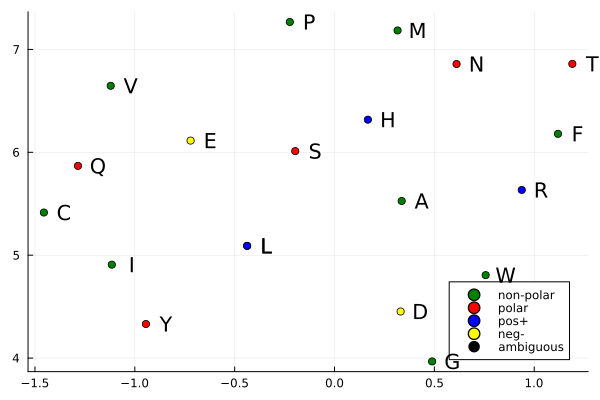
\includegraphics[width=\textwidth]{ur50tr_emb}
        \caption{Made starting from random hyperdimensional vectors for each amino acid, $k=50$.}
        \label{fig:AAtr50ru}
    \end{subfigure}
    
    \begin{subfigure}{0.48\textwidth}
        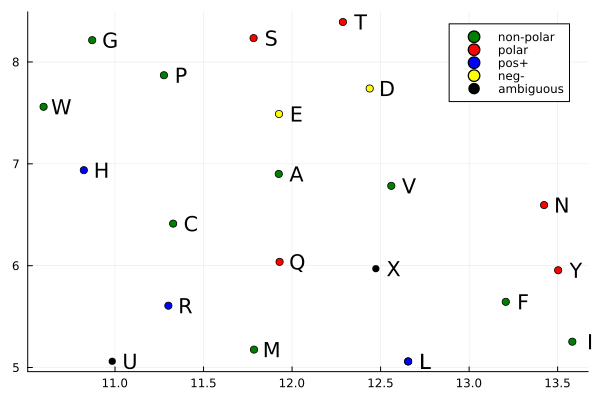
\includegraphics[width=\textwidth]{u4tr_emb}
        \caption{Made starting from extended ESM-2 embeddings for each amino acid, $k=4$.}
        \label{fig:AAtr4u}
    \end{subfigure}
    \hfill
    \begin{subfigure}{0.48\textwidth}
        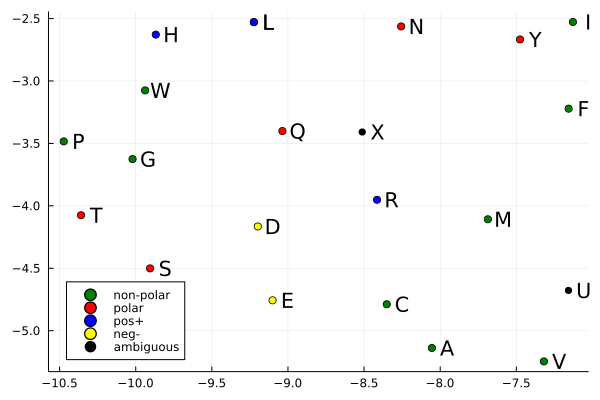
\includegraphics[width=\textwidth]{u50tr_emb}
        \caption{Made starting from extended ESM-2 embeddings for each amino acid, $k=50$.}
        \label{fig:AAtr50u}
    \end{subfigure}
    \caption{Scatter plot of a two-dimensional UMAP projection of the average amino acid HDVs with neighborhood-information of $k$ encoded. Learned from the human reference proteome. The amino acids are annotated and colored based on their chemical property of polarity.}
    \label{fig:main3}
\end{figure}

\begin{table}[h!]
    \label{tbl:target_grant}
    \caption{Target similarities made from Grantham's distance matrix}
    \resizebox{\textwidth}{!}{\begin{tabular}{cccccccccccccccccccc}
        $0.0$ & $0.73$ & $0.87$ & $0.8$ & $0.87$ & $0.73$ & $0.87$ & $0.8$ & $0.8$ & $0.8$ & $0.8$ & $0.87$ & $0.8$ & $0.8$ & $0.8$ & $0.67$ & $0.73$ & $0.73$ & $0.93$ & $0.87$\\ \hline
        $0.73$ & $0.0$ & $0.93$ & $1.0$ & $0.87$ & $0.93$ & $0.93$ & $0.8$ & $0.93$ & $0.8$ & $0.8$ & $0.93$ & $0.93$ & $0.93$ & $0.93$ & $0.8$ & $0.8$ & $0.8$ & $0.87$ & $0.87$\\ \hline
        $0.87$ & $0.93$ & $0.0$ & $0.6$ & $0.93$ & $0.8$ & $0.8$ & $0.93$ & $0.8$ & $1.0$ & $0.93$ & $0.67$ & $0.8$ & $0.73$ & $0.87$ & $0.73$ & $0.8$ & $0.93$ & $1.0$ & $0.93$\\ \hline
        $0.8$ & $1.0$ & $0.6$ & $0.0$ & $0.93$ & $0.87$ & $0.73$ & $0.93$ & $0.67$ & $0.93$ & $0.87$ & $0.73$ & $0.8$ & $0.6$ & $0.73$ & $0.73$ & $0.8$ & $0.87$ & $0.93$ & $0.87$\\ \hline
        $0.87$ & $0.87$ & $0.93$ & $0.93$ & $0.0$ & $0.93$ & $0.8$ & $0.73$ & $0.93$ & $0.73$ & $0.73$ & $0.93$ & $1.0$ & $0.93$ & $0.93$ & $0.87$ & $0.87$ & $0.8$ & $0.67$ & $0.53$\\ \hline
        $0.73$ & $0.93$ & $0.8$ & $0.87$ & $0.93$ & $0.0$ & $0.87$ & $1.0$ & $0.87$ & $1.0$ & $0.93$ & $0.73$ & $0.87$ & $0.87$ & $0.87$ & $0.73$ & $0.87$ & $0.93$ & $0.87$ & $0.93$\\ \hline
        $0.87$ & $0.93$ & $0.8$ & $0.73$ & $0.8$ & $0.87$ & $0.0$ & $0.93$ & $0.8$ & $0.93$ & $0.87$ & $0.67$ & $0.87$ & $0.73$ & $0.73$ & $0.8$ & $0.87$ & $0.93$ & $0.87$ & $0.6$\\ \hline
        $0.8$ & $0.8$ & $0.93$ & $0.93$ & $0.73$ & $1.0$ & $0.93$ & $0.0$ & $0.93$ & $0.6$ & $0.67$ & $0.93$ & $0.93$ & $0.93$ & $0.93$ & $0.87$ & $0.8$ & $0.53$ & $0.93$ & $0.8$\\ \hline
        $0.8$ & $0.93$ & $0.8$ & $0.67$ & $0.93$ & $0.87$ & $0.8$ & $0.93$ & $0.0$ & $0.87$ & $0.8$ & $0.73$ & $0.8$ & $0.67$ & $0.6$ & $0.73$ & $0.8$ & $0.87$ & $0.93$ & $0.87$\\ \hline
        $0.8$ & $0.8$ & $1.0$ & $0.93$ & $0.73$ & $1.0$ & $0.93$ & $0.6$ & $0.87$ & $0.0$ & $0.6$ & $0.93$ & $0.93$ & $0.87$ & $0.87$ & $0.87$ & $0.8$ & $0.67$ & $0.87$ & $0.8$\\ \hline
        $0.8$ & $0.8$ & $0.93$ & $0.87$ & $0.73$ & $0.93$ & $0.87$ & $0.67$ & $0.8$ & $0.6$ & $0.0$ & $0.87$ & $0.87$ & $0.73$ & $0.8$ & $0.8$ & $0.8$ & $0.67$ & $0.8$ & $0.8$\\ \hline
        $0.87$ & $0.93$ & $0.67$ & $0.73$ & $0.93$ & $0.73$ & $0.67$ & $0.93$ & $0.73$ & $0.93$ & $0.87$ & $0.0$ & $0.87$ & $0.73$ & $0.73$ & $0.67$ & $0.73$ & $0.93$ & $1.0$ & $0.87$\\ \hline
        $0.8$ & $0.93$ & $0.8$ & $0.8$ & $1.0$ & $0.87$ & $0.87$ & $0.93$ & $0.8$ & $0.93$ & $0.87$ & $0.87$ & $0.0$ & $0.8$ & $0.87$ & $0.8$ & $0.8$ & $0.87$ & $1.0$ & $0.93$\\ \hline
        $0.8$ & $0.93$ & $0.73$ & $0.6$ & $0.93$ & $0.87$ & $0.73$ & $0.93$ & $0.67$ & $0.87$ & $0.73$ & $0.73$ & $0.8$ & $0.0$ & $0.67$ & $0.73$ & $0.8$ & $0.87$ & $0.87$ & $0.8$\\ \hline
        $0.8$ & $0.93$ & $0.87$ & $0.73$ & $0.93$ & $0.87$ & $0.73$ & $0.93$ & $0.6$ & $0.87$ & $0.8$ & $0.73$ & $0.87$ & $0.67$ & $0.0$ & $0.8$ & $0.8$ & $0.93$ & $0.93$ & $0.87$\\ \hline
        $0.67$ & $0.8$ & $0.73$ & $0.73$ & $0.87$ & $0.73$ & $0.8$ & $0.87$ & $0.73$ & $0.87$ & $0.8$ & $0.67$ & $0.8$ & $0.73$ & $0.8$ & $0.0$ & $0.67$ & $0.87$ & $0.93$ & $0.87$\\ \hline
        $0.73$ & $0.8$ & $0.8$ & $0.8$ & $0.87$ & $0.87$ & $0.87$ & $0.8$ & $0.8$ & $0.8$ & $0.8$ & $0.73$ & $0.8$ & $0.8$ & $0.8$ & $0.67$ & $0.0$ & $0.73$ & $0.87$ & $0.87$\\ \hline
        $0.73$ & $0.8$ & $0.93$ & $0.87$ & $0.8$ & $0.93$ & $0.93$ & $0.53$ & $0.87$ & $0.67$ & $0.67$ & $0.93$ & $0.87$ & $0.87$ & $0.93$ & $0.87$ & $0.73$ & $0.0$ & $0.93$ & $0.8$\\ \hline
        $0.93$ & $0.87$ & $1.0$ & $0.93$ & $0.67$ & $0.87$ & $0.87$ & $0.93$ & $0.93$ & $0.87$ & $0.8$ & $1.0$ & $1.0$ & $0.87$ & $0.93$ & $0.93$ & $0.87$ & $0.93$ & $0.0$ & $0.6$\\ \hline
        $0.87$ & $0.87$ & $0.93$ & $0.87$ & $0.53$ & $0.93$ & $0.6$ & $0.8$ & $0.87$ & $0.8$ & $0.8$ & $0.87$ & $0.93$ & $0.8$ & $0.87$ & $0.87$ & $0.87$ & $0.8$ & $0.6$ & $0.0$
        \end{tabular}}
\end{table}

\begin{table}[h!]
    \label{tbl:achieved_grant}
    \caption{Achieved similarities targeting Grantham's distance matrix}
    \resizebox{\textwidth}{!}{\begin{tabular}{cccccccccccccccccccc}
        $0.0$ & $0.49$ & $0.49$ & $0.48$ & $0.48$ & $0.49$ & $0.5$ & $0.49$ & $0.49$ & $0.5$ & $0.49$ & $0.49$ & $0.49$ & $0.49$ & $0.49$ & $0.48$ & $0.5$ & $0.51$ & $0.49$ & $0.49$\\ \hline
$0.49$ & $0.0$ & $0.49$ & $0.5$ & $0.49$ & $0.49$ & $0.49$ & $0.5$ & $0.5$ & $0.48$ & $0.5$ & $0.5$ & $0.5$ & $0.49$ & $0.48$ & $0.49$ & $0.49$ & $0.49$ & $0.49$ & $0.49$\\ \hline
$0.49$ & $0.49$ & $0.0$ & $0.49$ & $0.49$ & $0.49$ & $0.49$ & $0.49$ & $0.49$ & $0.5$ & $0.49$ & $0.49$ & $0.5$ & $0.49$ & $0.49$ & $0.5$ & $0.49$ & $0.5$ & $0.49$ & $0.49$\\ \hline
$0.48$ & $0.5$ & $0.49$ & $0.0$ & $0.49$ & $0.48$ & $0.5$ & $0.5$ & $0.49$ & $0.49$ & $0.49$ & $0.5$ & $0.5$ & $0.5$ & $0.49$ & $0.5$ & $0.49$ & $0.49$ & $0.49$ & $0.49$\\ \hline
$0.48$ & $0.49$ & $0.49$ & $0.49$ & $0.0$ & $0.5$ & $0.5$ & $0.5$ & $0.49$ & $0.49$ & $0.5$ & $0.5$ & $0.5$ & $0.49$ & $0.5$ & $0.5$ & $0.51$ & $0.51$ & $0.5$ & $0.49$\\ \hline
$0.49$ & $0.49$ & $0.49$ & $0.48$ & $0.5$ & $0.0$ & $0.5$ & $0.49$ & $0.5$ & $0.49$ & $0.49$ & $0.5$ & $0.49$ & $0.49$ & $0.49$ & $0.5$ & $0.5$ & $0.49$ & $0.5$ & $0.5$\\ \hline
$0.5$ & $0.49$ & $0.49$ & $0.5$ & $0.5$ & $0.5$ & $0.0$ & $0.5$ & $0.51$ & $0.5$ & $0.5$ & $0.5$ & $0.5$ & $0.49$ & $0.49$ & $0.49$ & $0.49$ & $0.5$ & $0.48$ & $0.49$\\ \hline
$0.49$ & $0.5$ & $0.49$ & $0.5$ & $0.5$ & $0.49$ & $0.5$ & $0.0$ & $0.48$ & $0.49$ & $0.49$ & $0.51$ & $0.5$ & $0.5$ & $0.49$ & $0.5$ & $0.49$ & $0.5$ & $0.5$ & $0.5$\\ \hline
$0.49$ & $0.5$ & $0.49$ & $0.49$ & $0.49$ & $0.5$ & $0.51$ & $0.48$ & $0.0$ & $0.5$ & $0.49$ & $0.5$ & $0.5$ & $0.49$ & $0.5$ & $0.5$ & $0.48$ & $0.49$ & $0.49$ & $0.49$\\ \hline
$0.5$ & $0.48$ & $0.5$ & $0.49$ & $0.49$ & $0.49$ & $0.5$ & $0.49$ & $0.5$ & $0.0$ & $0.5$ & $0.5$ & $0.49$ & $0.49$ & $0.49$ & $0.49$ & $0.49$ & $0.5$ & $0.5$ & $0.48$\\ \hline
$0.49$ & $0.5$ & $0.49$ & $0.49$ & $0.5$ & $0.49$ & $0.5$ & $0.49$ & $0.49$ & $0.5$ & $0.0$ & $0.49$ & $0.49$ & $0.51$ & $0.5$ & $0.49$ & $0.5$ & $0.5$ & $0.49$ & $0.49$\\ \hline
$0.49$ & $0.5$ & $0.49$ & $0.5$ & $0.5$ & $0.5$ & $0.5$ & $0.51$ & $0.5$ & $0.5$ & $0.49$ & $0.0$ & $0.5$ & $0.49$ & $0.5$ & $0.49$ & $0.5$ & $0.49$ & $0.5$ & $0.49$\\ \hline
$0.49$ & $0.5$ & $0.5$ & $0.5$ & $0.5$ & $0.49$ & $0.5$ & $0.5$ & $0.5$ & $0.49$ & $0.49$ & $0.5$ & $0.0$ & $0.49$ & $0.5$ & $0.49$ & $0.5$ & $0.49$ & $0.5$ & $0.48$\\ \hline
$0.49$ & $0.49$ & $0.49$ & $0.5$ & $0.49$ & $0.49$ & $0.49$ & $0.5$ & $0.49$ & $0.49$ & $0.51$ & $0.49$ & $0.49$ & $0.0$ & $0.49$ & $0.5$ & $0.5$ & $0.5$ & $0.49$ & $0.5$\\ \hline
$0.49$ & $0.48$ & $0.49$ & $0.49$ & $0.5$ & $0.49$ & $0.49$ & $0.49$ & $0.5$ & $0.49$ & $0.5$ & $0.5$ & $0.5$ & $0.49$ & $0.0$ & $0.49$ & $0.49$ & $0.49$ & $0.5$ & $0.5$\\ \hline
$0.48$ & $0.49$ & $0.5$ & $0.5$ & $0.5$ & $0.5$ & $0.49$ & $0.5$ & $0.5$ & $0.49$ & $0.49$ & $0.49$ & $0.49$ & $0.5$ & $0.49$ & $0.0$ & $0.49$ & $0.5$ & $0.49$ & $0.5$\\ \hline
$0.5$ & $0.49$ & $0.49$ & $0.49$ & $0.51$ & $0.5$ & $0.49$ & $0.49$ & $0.48$ & $0.49$ & $0.5$ & $0.5$ & $0.5$ & $0.5$ & $0.49$ & $0.49$ & $0.0$ & $0.5$ & $0.5$ & $0.5$\\ \hline
$0.51$ & $0.49$ & $0.5$ & $0.49$ & $0.51$ & $0.49$ & $0.5$ & $0.5$ & $0.49$ & $0.5$ & $0.5$ & $0.49$ & $0.49$ & $0.5$ & $0.49$ & $0.5$ & $0.5$ & $0.0$ & $0.49$ & $0.48$\\ \hline
$0.49$ & $0.49$ & $0.49$ & $0.49$ & $0.5$ & $0.5$ & $0.48$ & $0.5$ & $0.49$ & $0.5$ & $0.49$ & $0.5$ & $0.5$ & $0.49$ & $0.5$ & $0.49$ & $0.5$ & $0.49$ & $0.0$ & $0.5$\\ \hline
$0.49$ & $0.49$ & $0.49$ & $0.49$ & $0.49$ & $0.5$ & $0.49$ & $0.5$ & $0.49$ & $0.48$ & $0.49$ & $0.49$ & $0.48$ & $0.5$ & $0.5$ & $0.5$ & $0.5$ & $0.48$ & $0.5$ & $0.0$
\end{tabular}}
\end{table}

\begin{table}[h!]
    \label{tbl:target_blo}
    \caption{Target similarities made from BLOSUM62 matrix}
    \resizebox{\textwidth}{!}{\begin{tabular}{cccccccccccccccccccc}
        $0.0$ & $0.73$ & $0.87$ & $0.8$ & $0.87$ & $0.73$ & $0.87$ & $0.8$ & $0.8$ & $0.8$ & $0.8$ & $0.87$ & $0.8$ & $0.8$ & $0.8$ & $0.67$ & $0.73$ & $0.73$ & $0.93$ & $0.87$\\ \hline
$0.73$ & $0.0$ & $0.93$ & $1.0$ & $0.87$ & $0.93$ & $0.93$ & $0.8$ & $0.93$ & $0.8$ & $0.8$ & $0.93$ & $0.93$ & $0.93$ & $0.93$ & $0.8$ & $0.8$ & $0.8$ & $0.87$ & $0.87$\\ \hline
$0.87$ & $0.93$ & $0.0$ & $0.6$ & $0.93$ & $0.8$ & $0.8$ & $0.93$ & $0.8$ & $1.0$ & $0.93$ & $0.67$ & $0.8$ & $0.73$ & $0.87$ & $0.73$ & $0.8$ & $0.93$ & $1.0$ & $0.93$\\ \hline
$0.8$ & $1.0$ & $0.6$ & $0.0$ & $0.93$ & $0.87$ & $0.73$ & $0.93$ & $0.67$ & $0.93$ & $0.87$ & $0.73$ & $0.8$ & $0.6$ & $0.73$ & $0.73$ & $0.8$ & $0.87$ & $0.93$ & $0.87$\\ \hline
$0.87$ & $0.87$ & $0.93$ & $0.93$ & $0.0$ & $0.93$ & $0.8$ & $0.73$ & $0.93$ & $0.73$ & $0.73$ & $0.93$ & $1.0$ & $0.93$ & $0.93$ & $0.87$ & $0.87$ & $0.8$ & $0.67$ & $0.53$\\ \hline
$0.73$ & $0.93$ & $0.8$ & $0.87$ & $0.93$ & $0.0$ & $0.87$ & $1.0$ & $0.87$ & $1.0$ & $0.93$ & $0.73$ & $0.87$ & $0.87$ & $0.87$ & $0.73$ & $0.87$ & $0.93$ & $0.87$ & $0.93$\\ \hline
$0.87$ & $0.93$ & $0.8$ & $0.73$ & $0.8$ & $0.87$ & $0.0$ & $0.93$ & $0.8$ & $0.93$ & $0.87$ & $0.67$ & $0.87$ & $0.73$ & $0.73$ & $0.8$ & $0.87$ & $0.93$ & $0.87$ & $0.6$\\ \hline
$0.8$ & $0.8$ & $0.93$ & $0.93$ & $0.73$ & $1.0$ & $0.93$ & $0.0$ & $0.93$ & $0.6$ & $0.67$ & $0.93$ & $0.93$ & $0.93$ & $0.93$ & $0.87$ & $0.8$ & $0.53$ & $0.93$ & $0.8$\\ \hline
$0.8$ & $0.93$ & $0.8$ & $0.67$ & $0.93$ & $0.87$ & $0.8$ & $0.93$ & $0.0$ & $0.87$ & $0.8$ & $0.73$ & $0.8$ & $0.67$ & $0.6$ & $0.73$ & $0.8$ & $0.87$ & $0.93$ & $0.87$\\ \hline
$0.8$ & $0.8$ & $1.0$ & $0.93$ & $0.73$ & $1.0$ & $0.93$ & $0.6$ & $0.87$ & $0.0$ & $0.6$ & $0.93$ & $0.93$ & $0.87$ & $0.87$ & $0.87$ & $0.8$ & $0.67$ & $0.87$ & $0.8$\\ \hline
$0.8$ & $0.8$ & $0.93$ & $0.87$ & $0.73$ & $0.93$ & $0.87$ & $0.67$ & $0.8$ & $0.6$ & $0.0$ & $0.87$ & $0.87$ & $0.73$ & $0.8$ & $0.8$ & $0.8$ & $0.67$ & $0.8$ & $0.8$\\ \hline
$0.87$ & $0.93$ & $0.67$ & $0.73$ & $0.93$ & $0.73$ & $0.67$ & $0.93$ & $0.73$ & $0.93$ & $0.87$ & $0.0$ & $0.87$ & $0.73$ & $0.73$ & $0.67$ & $0.73$ & $0.93$ & $1.0$ & $0.87$\\ \hline
$0.8$ & $0.93$ & $0.8$ & $0.8$ & $1.0$ & $0.87$ & $0.87$ & $0.93$ & $0.8$ & $0.93$ & $0.87$ & $0.87$ & $0.0$ & $0.8$ & $0.87$ & $0.8$ & $0.8$ & $0.87$ & $1.0$ & $0.93$\\ \hline
$0.8$ & $0.93$ & $0.73$ & $0.6$ & $0.93$ & $0.87$ & $0.73$ & $0.93$ & $0.67$ & $0.87$ & $0.73$ & $0.73$ & $0.8$ & $0.0$ & $0.67$ & $0.73$ & $0.8$ & $0.87$ & $0.87$ & $0.8$\\ \hline
$0.8$ & $0.93$ & $0.87$ & $0.73$ & $0.93$ & $0.87$ & $0.73$ & $0.93$ & $0.6$ & $0.87$ & $0.8$ & $0.73$ & $0.87$ & $0.67$ & $0.0$ & $0.8$ & $0.8$ & $0.93$ & $0.93$ & $0.87$\\ \hline
$0.67$ & $0.8$ & $0.73$ & $0.73$ & $0.87$ & $0.73$ & $0.8$ & $0.87$ & $0.73$ & $0.87$ & $0.8$ & $0.67$ & $0.8$ & $0.73$ & $0.8$ & $0.0$ & $0.67$ & $0.87$ & $0.93$ & $0.87$\\ \hline
$0.73$ & $0.8$ & $0.8$ & $0.8$ & $0.87$ & $0.87$ & $0.87$ & $0.8$ & $0.8$ & $0.8$ & $0.8$ & $0.73$ & $0.8$ & $0.8$ & $0.8$ & $0.67$ & $0.0$ & $0.73$ & $0.87$ & $0.87$\\ \hline
$0.73$ & $0.8$ & $0.93$ & $0.87$ & $0.8$ & $0.93$ & $0.93$ & $0.53$ & $0.87$ & $0.67$ & $0.67$ & $0.93$ & $0.87$ & $0.87$ & $0.93$ & $0.87$ & $0.73$ & $0.0$ & $0.93$ & $0.8$\\ \hline
$0.93$ & $0.87$ & $1.0$ & $0.93$ & $0.67$ & $0.87$ & $0.87$ & $0.93$ & $0.93$ & $0.87$ & $0.8$ & $1.0$ & $1.0$ & $0.87$ & $0.93$ & $0.93$ & $0.87$ & $0.93$ & $0.0$ & $0.6$\\ \hline
$0.87$ & $0.87$ & $0.93$ & $0.87$ & $0.53$ & $0.93$ & $0.6$ & $0.8$ & $0.87$ & $0.8$ & $0.8$ & $0.87$ & $0.93$ & $0.8$ & $0.87$ & $0.87$ & $0.87$ & $0.8$ & $0.6$ & $0.0$
        \end{tabular}}
\end{table}

\begin{table}[h!]
    \label{tbl:achieved_blo}
    \caption{Achieved similarities targeting BLOSUM62 matrix}
    \resizebox{\textwidth}{!}{\begin{tabular}{cccccccccccccccccccc}
        $0.0$ & $0.49$ & $0.49$ & $0.49$ & $0.5$ & $0.49$ & $0.48$ & $0.49$ & $0.5$ & $0.49$ & $0.5$ & $0.49$ & $0.5$ & $0.5$ & $0.5$ & $0.49$ & $0.49$ & $0.49$ & $0.49$ & $0.49$\\ \hline
$0.49$ & $0.0$ & $0.5$ & $0.5$ & $0.5$ & $0.49$ & $0.49$ & $0.49$ & $0.49$ & $0.49$ & $0.48$ & $0.49$ & $0.48$ & $0.49$ & $0.49$ & $0.49$ & $0.49$ & $0.49$ & $0.49$ & $0.49$\\ \hline
$0.49$ & $0.5$ & $0.0$ & $0.49$ & $0.5$ & $0.5$ & $0.5$ & $0.49$ & $0.51$ & $0.48$ & $0.49$ & $0.5$ & $0.49$ & $0.49$ & $0.5$ & $0.5$ & $0.48$ & $0.49$ & $0.49$ & $0.49$\\ \hline
$0.49$ & $0.5$ & $0.49$ & $0.0$ & $0.49$ & $0.5$ & $0.49$ & $0.5$ & $0.5$ & $0.5$ & $0.5$ & $0.49$ & $0.49$ & $0.51$ & $0.49$ & $0.49$ & $0.49$ & $0.49$ & $0.48$ & $0.49$\\ \hline
$0.5$ & $0.5$ & $0.5$ & $0.49$ & $0.0$ & $0.5$ & $0.5$ & $0.51$ & $0.5$ & $0.5$ & $0.5$ & $0.5$ & $0.5$ & $0.49$ & $0.5$ & $0.49$ & $0.5$ & $0.49$ & $0.5$ & $0.48$\\ \hline
$0.49$ & $0.49$ & $0.5$ & $0.5$ & $0.5$ & $0.0$ & $0.49$ & $0.49$ & $0.5$ & $0.5$ & $0.5$ & $0.49$ & $0.49$ & $0.49$ & $0.5$ & $0.49$ & $0.5$ & $0.49$ & $0.49$ & $0.5$\\ \hline
$0.48$ & $0.49$ & $0.5$ & $0.49$ & $0.5$ & $0.49$ & $0.0$ & $0.5$ & $0.49$ & $0.49$ & $0.5$ & $0.5$ & $0.5$ & $0.5$ & $0.49$ & $0.5$ & $0.49$ & $0.49$ & $0.49$ & $0.49$\\ \hline
$0.49$ & $0.49$ & $0.49$ & $0.5$ & $0.51$ & $0.49$ & $0.5$ & $0.0$ & $0.5$ & $0.5$ & $0.5$ & $0.5$ & $0.5$ & $0.5$ & $0.5$ & $0.5$ & $0.49$ & $0.49$ & $0.49$ & $0.5$\\ \hline
$0.5$ & $0.49$ & $0.51$ & $0.5$ & $0.5$ & $0.5$ & $0.49$ & $0.5$ & $0.0$ & $0.49$ & $0.5$ & $0.49$ & $0.49$ & $0.5$ & $0.5$ & $0.49$ & $0.49$ & $0.5$ & $0.49$ & $0.48$\\ \hline
$0.49$ & $0.49$ & $0.48$ & $0.5$ & $0.5$ & $0.5$ & $0.49$ & $0.5$ & $0.49$ & $0.0$ & $0.5$ & $0.48$ & $0.49$ & $0.49$ & $0.49$ & $0.5$ & $0.49$ & $0.5$ & $0.48$ & $0.49$\\ \hline
$0.5$ & $0.48$ & $0.49$ & $0.5$ & $0.5$ & $0.5$ & $0.5$ & $0.5$ & $0.5$ & $0.5$ & $0.0$ & $0.5$ & $0.5$ & $0.5$ & $0.5$ & $0.49$ & $0.49$ & $0.49$ & $0.49$ & $0.49$\\ \hline
$0.49$ & $0.49$ & $0.5$ & $0.49$ & $0.5$ & $0.49$ & $0.5$ & $0.5$ & $0.49$ & $0.48$ & $0.5$ & $0.0$ & $0.51$ & $0.5$ & $0.49$ & $0.49$ & $0.49$ & $0.5$ & $0.49$ & $0.5$\\ \hline
$0.5$ & $0.48$ & $0.49$ & $0.49$ & $0.5$ & $0.49$ & $0.5$ & $0.5$ & $0.49$ & $0.49$ & $0.5$ & $0.51$ & $0.0$ & $0.5$ & $0.49$ & $0.49$ & $0.49$ & $0.49$ & $0.49$ & $0.49$\\ \hline
$0.5$ & $0.49$ & $0.49$ & $0.51$ & $0.49$ & $0.49$ & $0.5$ & $0.5$ & $0.5$ & $0.49$ & $0.5$ & $0.5$ & $0.5$ & $0.0$ & $0.5$ & $0.5$ & $0.5$ & $0.49$ & $0.5$ & $0.49$\\ \hline
$0.5$ & $0.49$ & $0.5$ & $0.49$ & $0.5$ & $0.5$ & $0.49$ & $0.5$ & $0.5$ & $0.49$ & $0.5$ & $0.49$ & $0.49$ & $0.5$ & $0.0$ & $0.5$ & $0.5$ & $0.49$ & $0.49$ & $0.49$\\ \hline
$0.49$ & $0.49$ & $0.5$ & $0.49$ & $0.49$ & $0.49$ & $0.5$ & $0.5$ & $0.49$ & $0.5$ & $0.49$ & $0.49$ & $0.49$ & $0.5$ & $0.5$ & $0.0$ & $0.49$ & $0.49$ & $0.49$ & $0.49$\\ \hline
$0.49$ & $0.49$ & $0.48$ & $0.49$ & $0.5$ & $0.5$ & $0.49$ & $0.49$ & $0.49$ & $0.49$ & $0.49$ & $0.49$ & $0.49$ & $0.5$ & $0.5$ & $0.49$ & $0.0$ & $0.49$ & $0.49$ & $0.49$\\ \hline
$0.49$ & $0.49$ & $0.49$ & $0.49$ & $0.49$ & $0.49$ & $0.49$ & $0.49$ & $0.5$ & $0.5$ & $0.49$ & $0.5$ & $0.49$ & $0.49$ & $0.49$ & $0.49$ & $0.49$ & $0.0$ & $0.49$ & $0.49$\\ \hline
$0.49$ & $0.49$ & $0.49$ & $0.48$ & $0.5$ & $0.49$ & $0.49$ & $0.49$ & $0.49$ & $0.48$ & $0.49$ & $0.49$ & $0.49$ & $0.5$ & $0.49$ & $0.49$ & $0.49$ & $0.49$ & $0.0$ & $0.49$\\ \hline
$0.49$ & $0.49$ & $0.49$ & $0.49$ & $0.48$ & $0.5$ & $0.49$ & $0.5$ & $0.48$ & $0.49$ & $0.49$ & $0.5$ & $0.49$ & $0.49$ & $0.49$ & $0.49$ & $0.49$ & $0.49$ & $0.49$ & $0.0$
\end{tabular}}
\end{table}
\chapter{Additional information on Chapter 5}\label{app:chp5}
\begin{figure}[H]
    \centering
    \begin{minipage}[b]{.6\textwidth}
        \begin{subfigure}[b]{\textwidth}
        \includegraphics[width=\textwidth]{loss_plot_25_8}
        \caption{Training losses}
        \label{fig:loss}
    \end{subfigure}
    \end{minipage}
    \\
    \centering
    \begin{minipage}[b]{.6\textwidth}
    \begin{subfigure}[b]{\textwidth}
        \includegraphics[width=\textwidth]{accuracy_plot_25_8}
        \caption{Accuracies}
        \label{fig:accuracy}
    \end{subfigure}
    \end{minipage}
    \\
    \centering
    \begin{minipage}[b]{.6\textwidth}
    \begin{subfigure}[b]{\textwidth}
        \includegraphics[width=\textwidth]{f1_plot_25_8}
        \caption{F1-scores}\label{fig:f1}
    \end{subfigure}
    \end{minipage}
    \caption{(a) cross-entropy losses (b) accuracies (c) F1-scores of all perceptron-based configurations tested. Trained with neighborhood-encodings of 60 \% of the training dataset of NetSurfP 2.0. Here $n=25$ and the secondary structure classification is dssp8-based. Note that the SLP and 1-layer MLP model was evaluated using fewer epochs than their 10-layer counterpart.}\label{fig:she2}
    \end{figure}

\begin{figure}[H]
        \centering
        \begin{minipage}[b]{.6\textwidth}
            \begin{subfigure}[b]{\textwidth}
            \includegraphics[width=\textwidth]{loss_plot_100_3}
            \caption{Training losses}
            \label{fig:loss}
        \end{subfigure}
        \end{minipage}
        \\
        \centering
        \begin{minipage}[b]{.6\textwidth}
        \begin{subfigure}[b]{\textwidth}
            \includegraphics[width=\textwidth]{accuracy_plot_100_3}
            \caption{Accuracies}
            \label{fig:accuracy}
        \end{subfigure}
        \end{minipage}
        \\
        \centering
        \begin{minipage}[b]{.6\textwidth}
        \begin{subfigure}[b]{\textwidth}
            \includegraphics[width=\textwidth]{f1_plot_100_3}
            \caption{F1-scores}\label{fig:f1}
        \end{subfigure}
        \end{minipage}
        \caption{(a) cross-entropy losses (b) accuracies (c) F1-scores of all perceptron-based configurations tested. Trained with neighborhood-encodings of 60 \% of the training dataset of NetSurfP 2.0. Here $n=100$ and the secondary structure classification is dssp3-based. Note that the SLP and 1-layer MLP model was evaluated using fewer epochs than their 10-layer counterpart.}\label{fig:she3}
        \end{figure}

        \begin{figure}[H]
            \centering
            \begin{minipage}[b]{.6\textwidth}
                \begin{subfigure}[b]{\textwidth}
                \includegraphics[width=\textwidth]{loss_plot_100_8}
                \caption{Training losses}
                \label{fig:loss}
            \end{subfigure}
            \end{minipage}
            \\
            \centering
            \begin{minipage}[b]{.6\textwidth}
            \begin{subfigure}[b]{\textwidth}
                \includegraphics[width=\textwidth]{accuracy_plot_100_8}
                \caption{Accuracies}
                \label{fig:accuracy}
            \end{subfigure}
            \end{minipage}
            \\
            \centering
            \begin{minipage}[b]{.6\textwidth}
            \begin{subfigure}[b]{\textwidth}
                \includegraphics[width=\textwidth]{f1_plot_100_8}
                \caption{F1-scores}\label{fig:f1}
            \end{subfigure}
            \end{minipage}
            \caption{(a) cross-entropy losses (b) accuracies (c) F1-scores of all perceptron-based configurations tested. Trained with neighborhood-encodings of 60 \% of the training dataset of NetSurfP 2.0. Here $n=100$ and the secondary structure classification is dssp8-based. Note that the SLP and 1-layer MLP model was evaluated using fewer epochs than their 10-layer counterpart.}\label{fig:she4}
            \end{figure}

\end{appendices}

\end{document}
